\section*{Divergence summaries}

\begin{figure*}[h]
    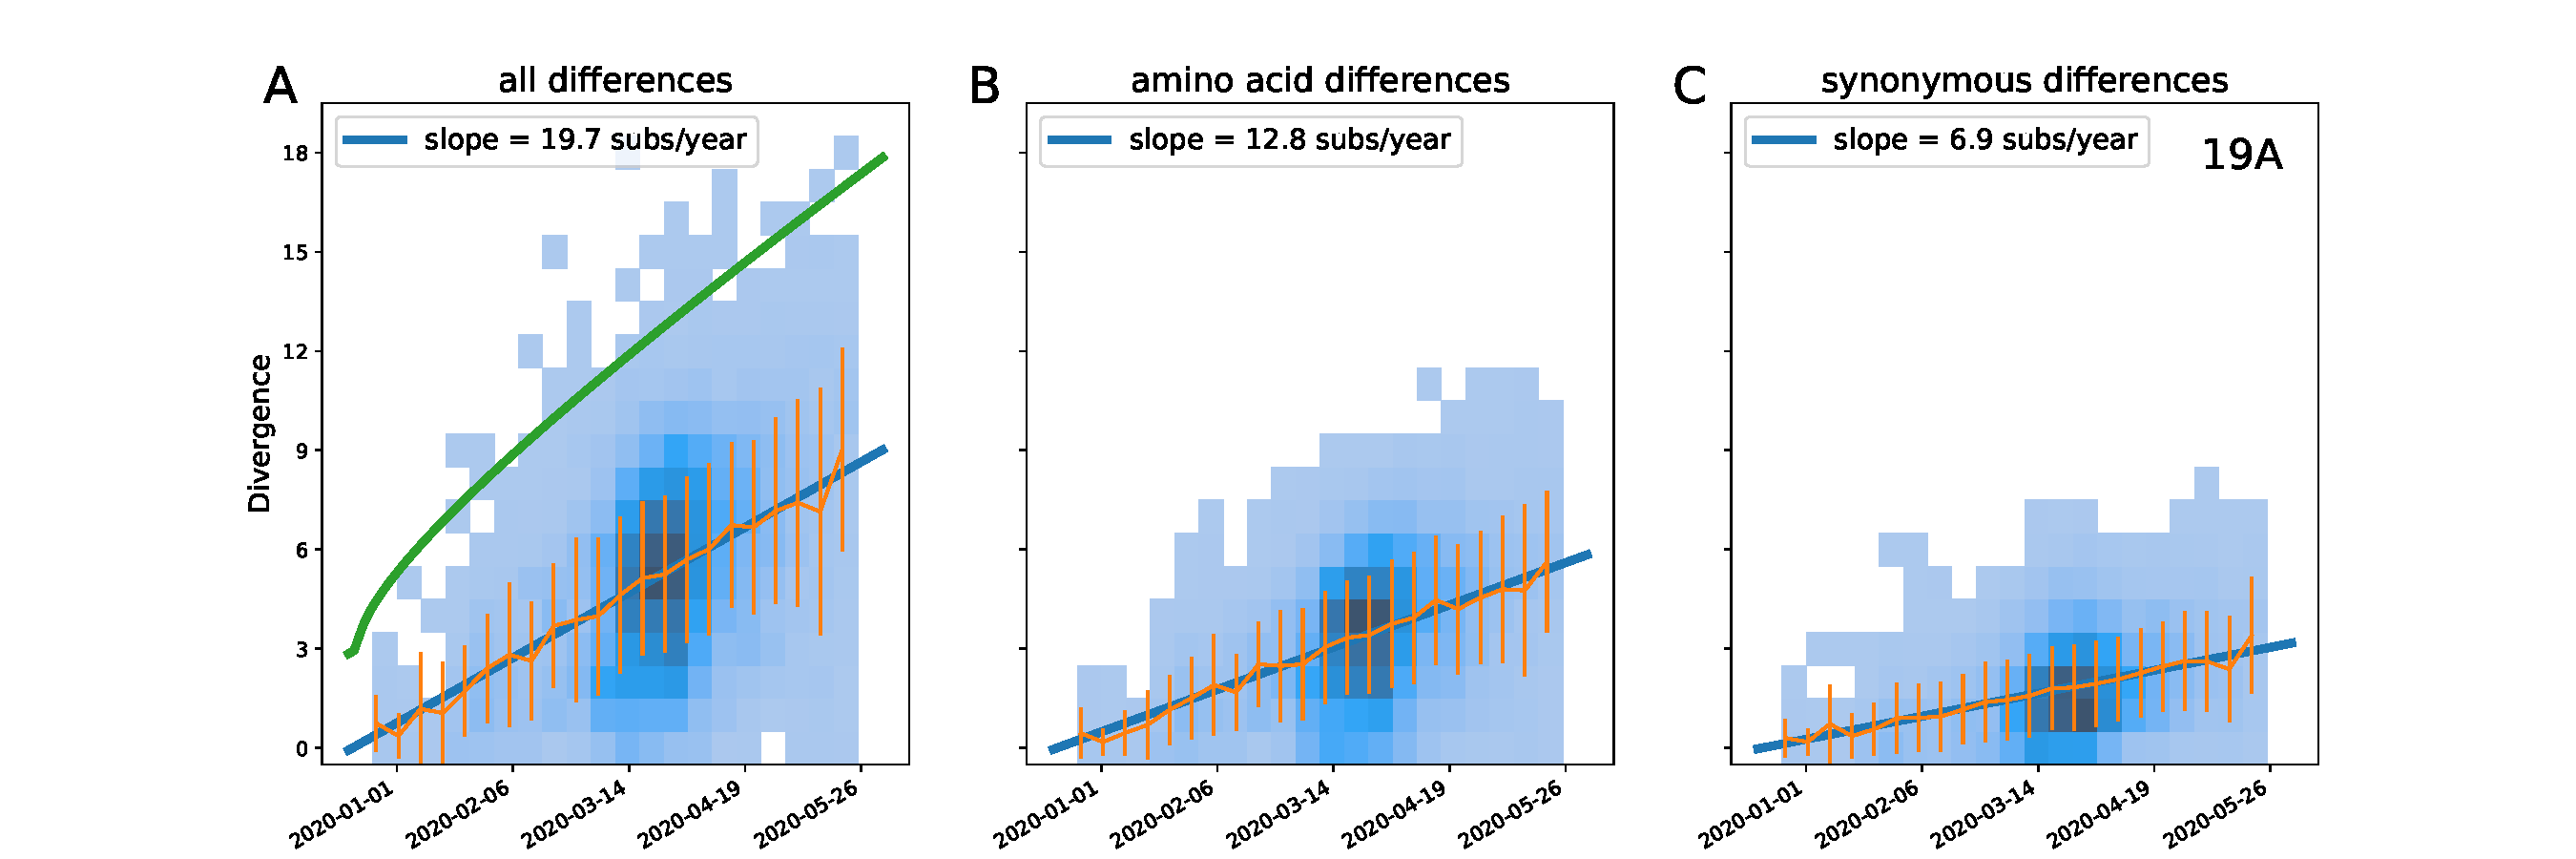
\includegraphics[width=0.8\textwidth]{figures/rtt/19A_rtt.pdf}
    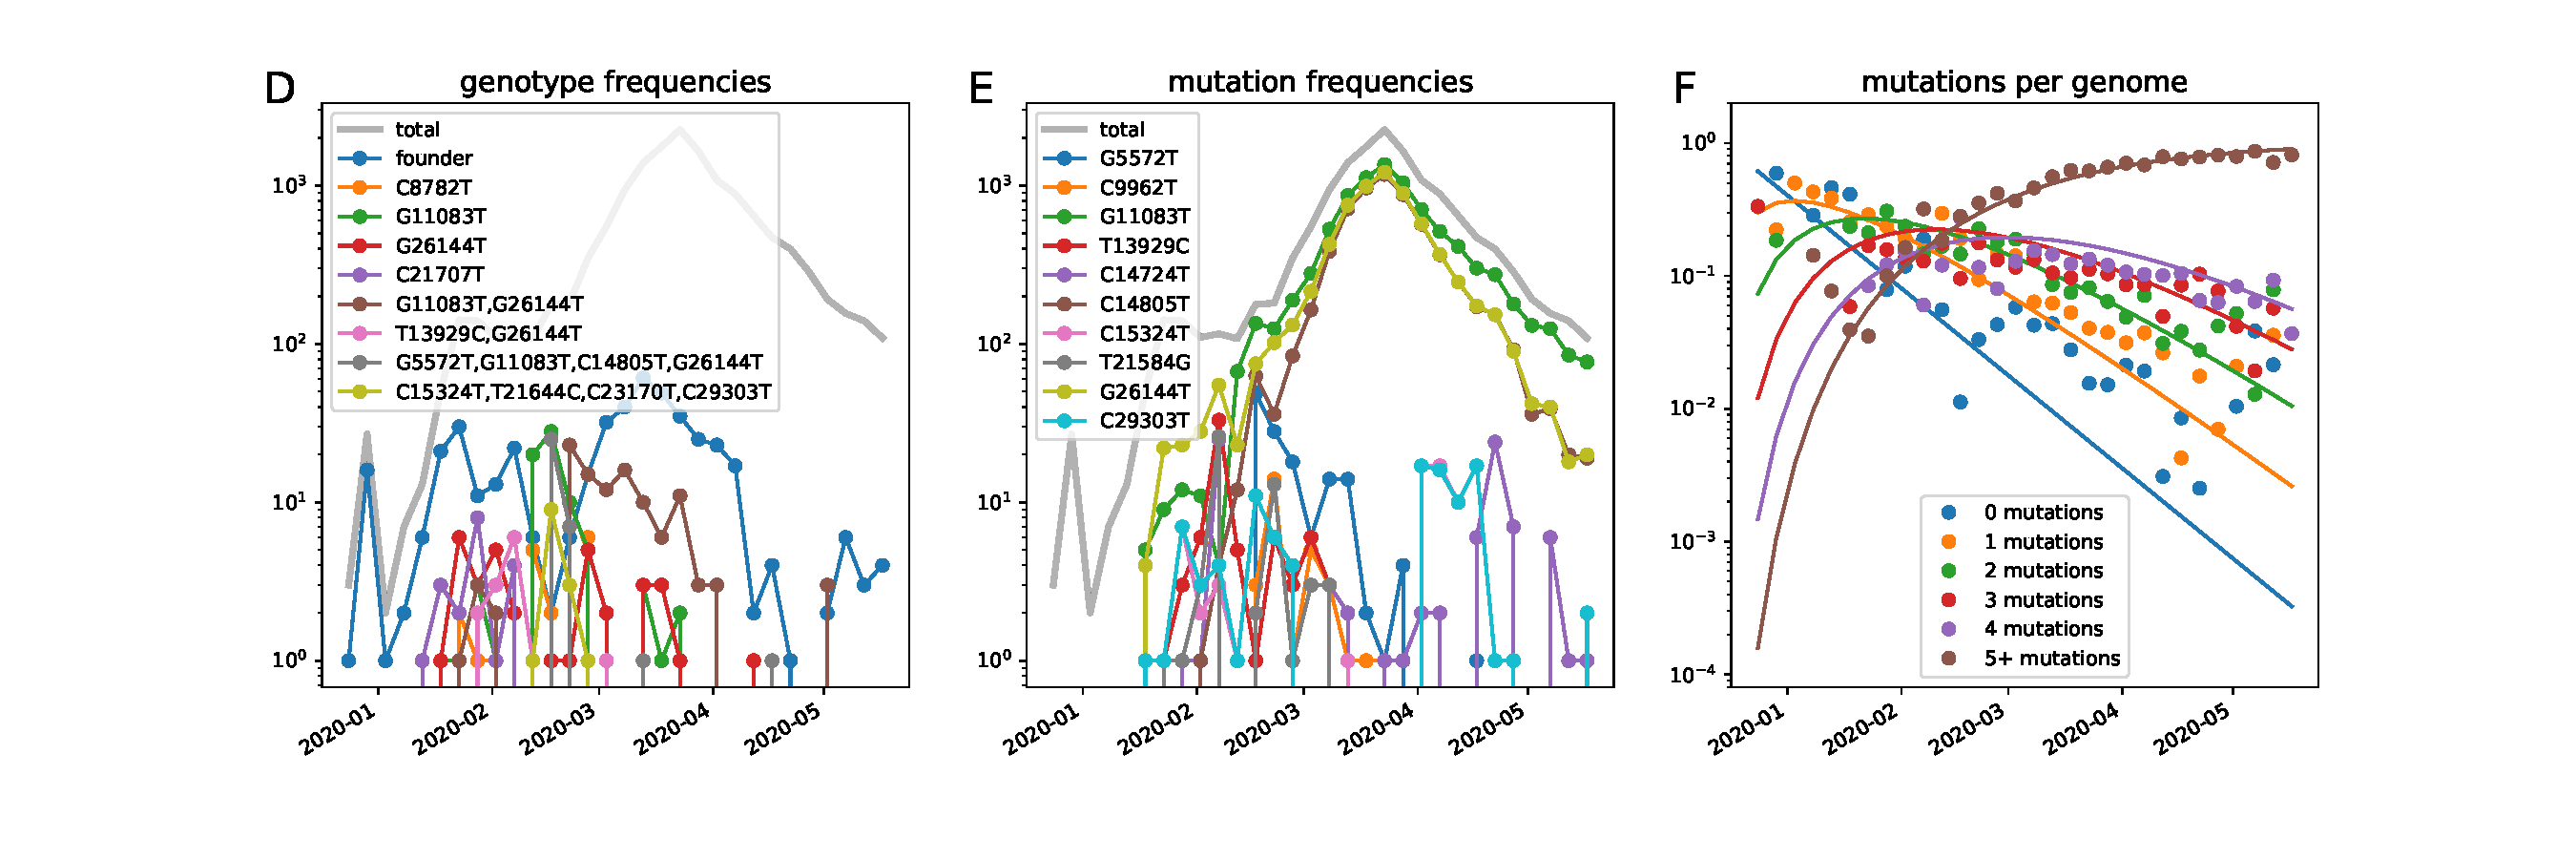
\includegraphics[width=0.8\textwidth]{figures/counts/19A_counts.pdf}
    \caption{{\bf Divergence increases linearly with time in clade 19A.}
    Top: Each panel shows the number of within-clade mutations (total (A), amino acid changing (B), synonymous (C)) as a function of time.
    The green line in panel A indicates the divergence cut-off, panels B\&C only show sequences that pass the divergence filter. Each panel also shows mean $\pm$ standard deviation and a weighted linear fit. Analogous figures for all clades considered are included in the appendix.
    Bottom: Panels D and E show the prevalence of specific genotypes (D) and specific mutations (E). In the case shown, the founder genotype initially dominates and no daughter genotype or mutation dominate. Panel F shows a Poisson model to the breakdown of the population into genotypes with different number of mutations over time.
    \label{fig:19A_divergence}}
\end{figure*}

\begin{figure*}[h]
    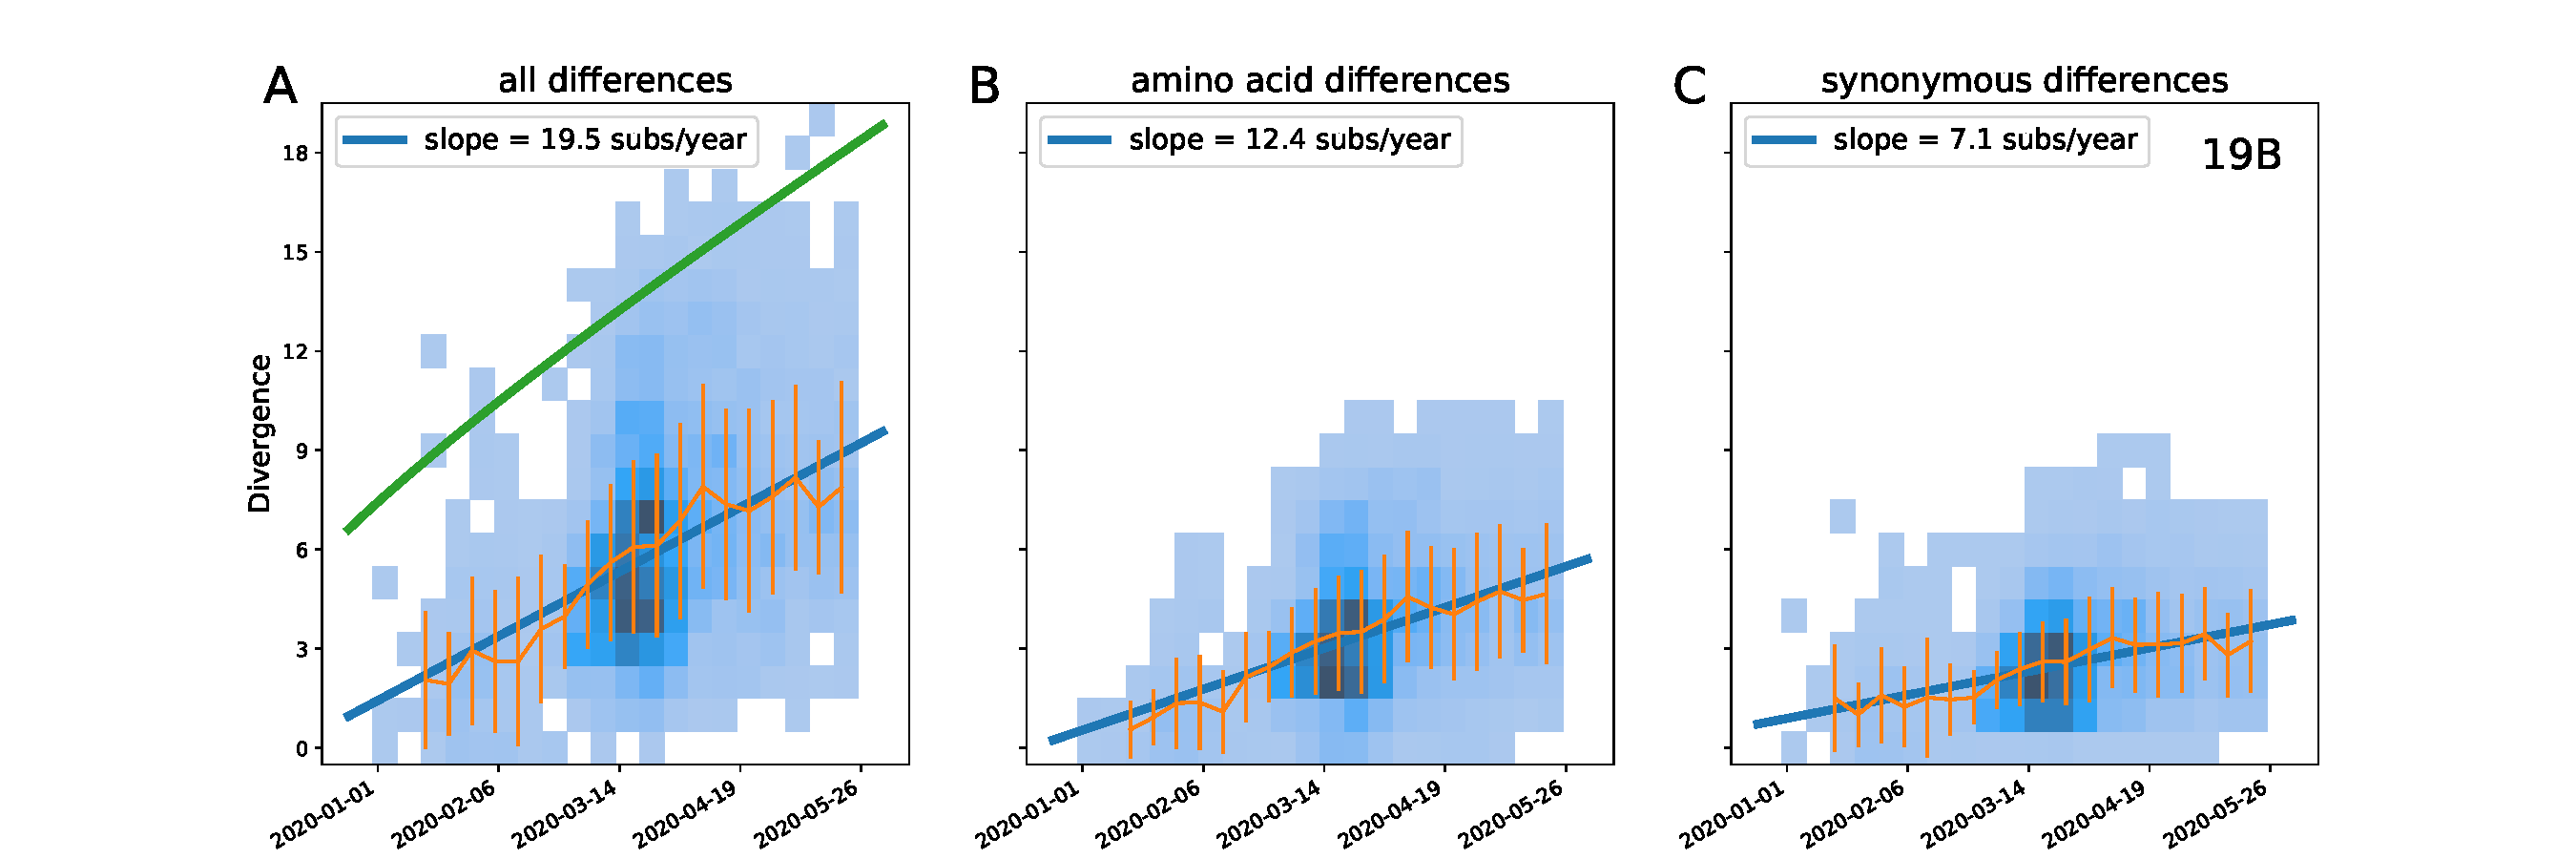
\includegraphics[width=0.8\textwidth]{figures/rtt/19B_rtt.pdf}
    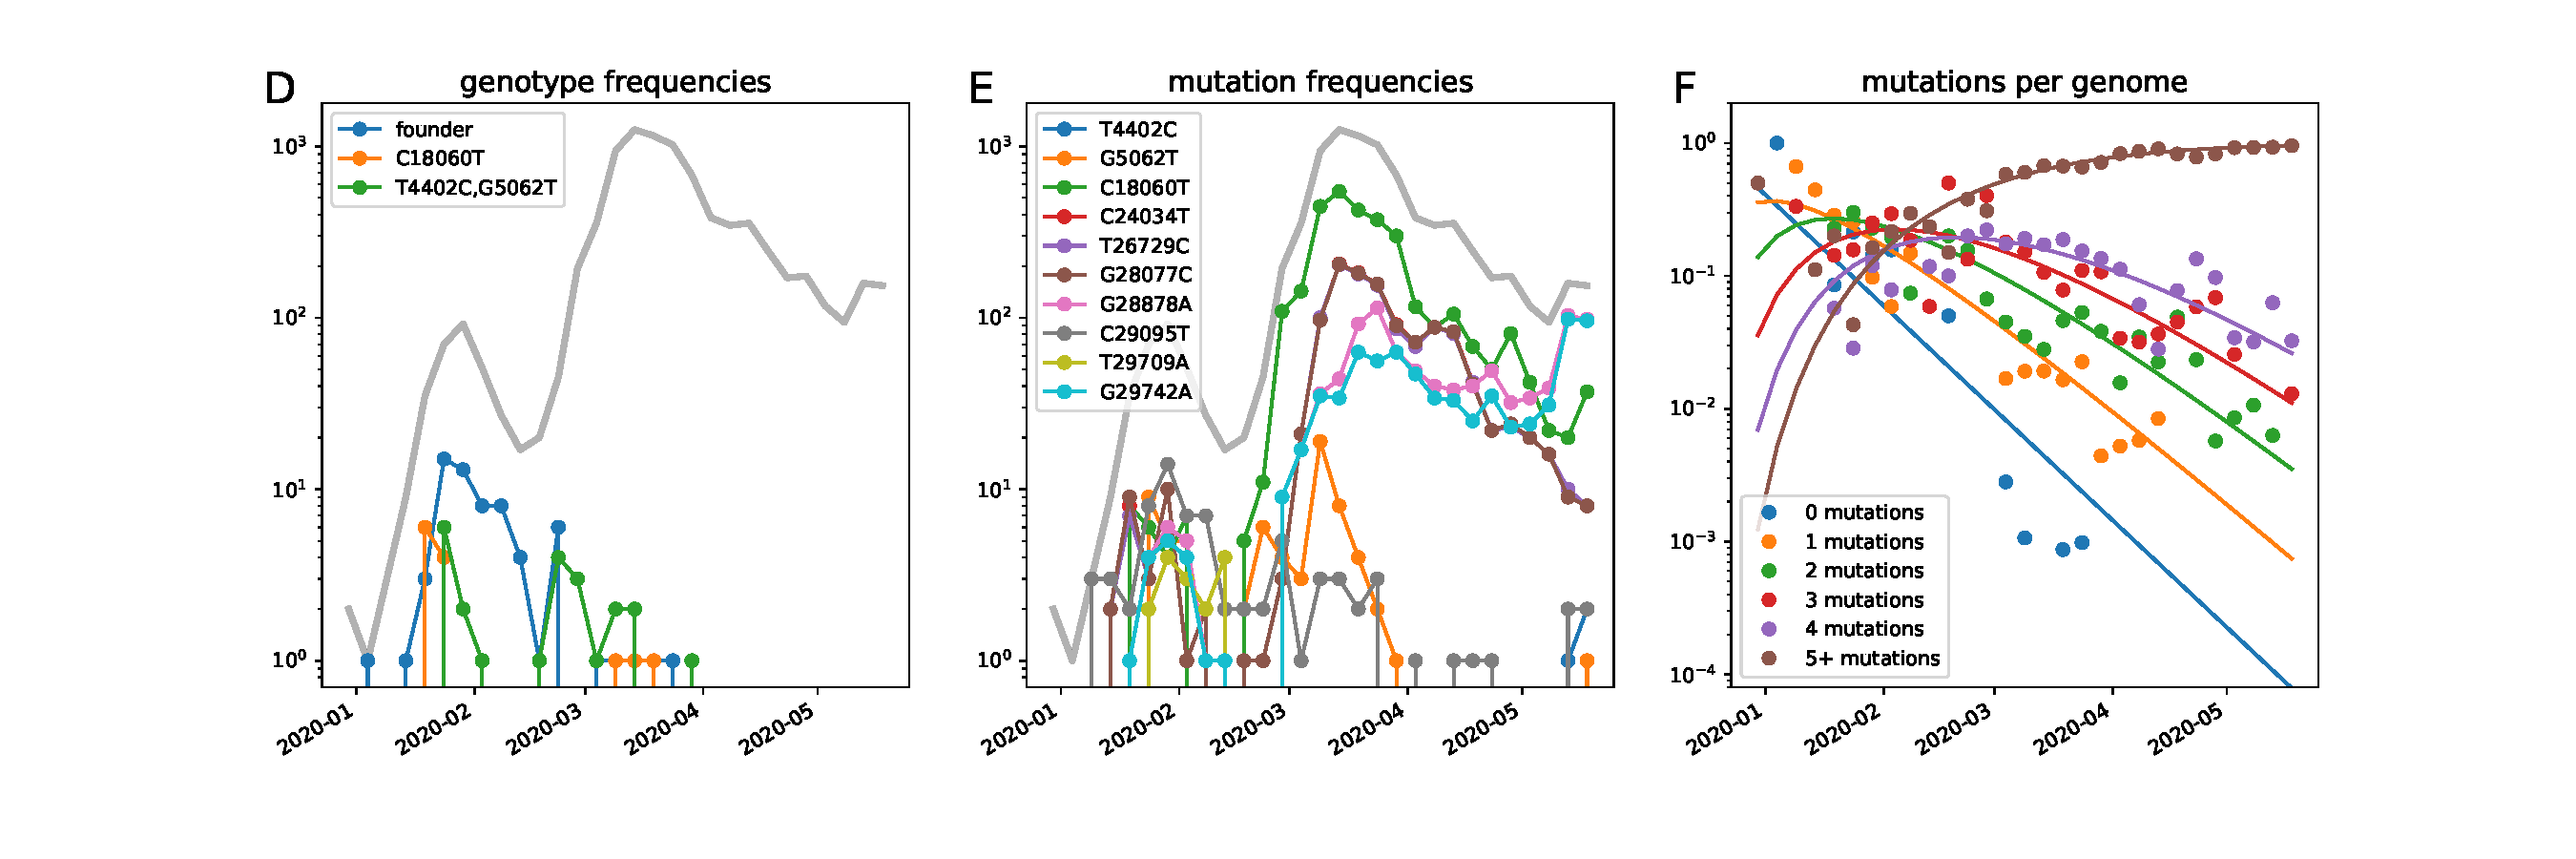
\includegraphics[width=0.8\textwidth]{figures/counts/19B_counts.pdf}
    \caption{{\bf Divergence increases linearly with time in clade 19B.}
    \label{fig:19B_divergence}}
\end{figure*}

\begin{figure*}[h]
    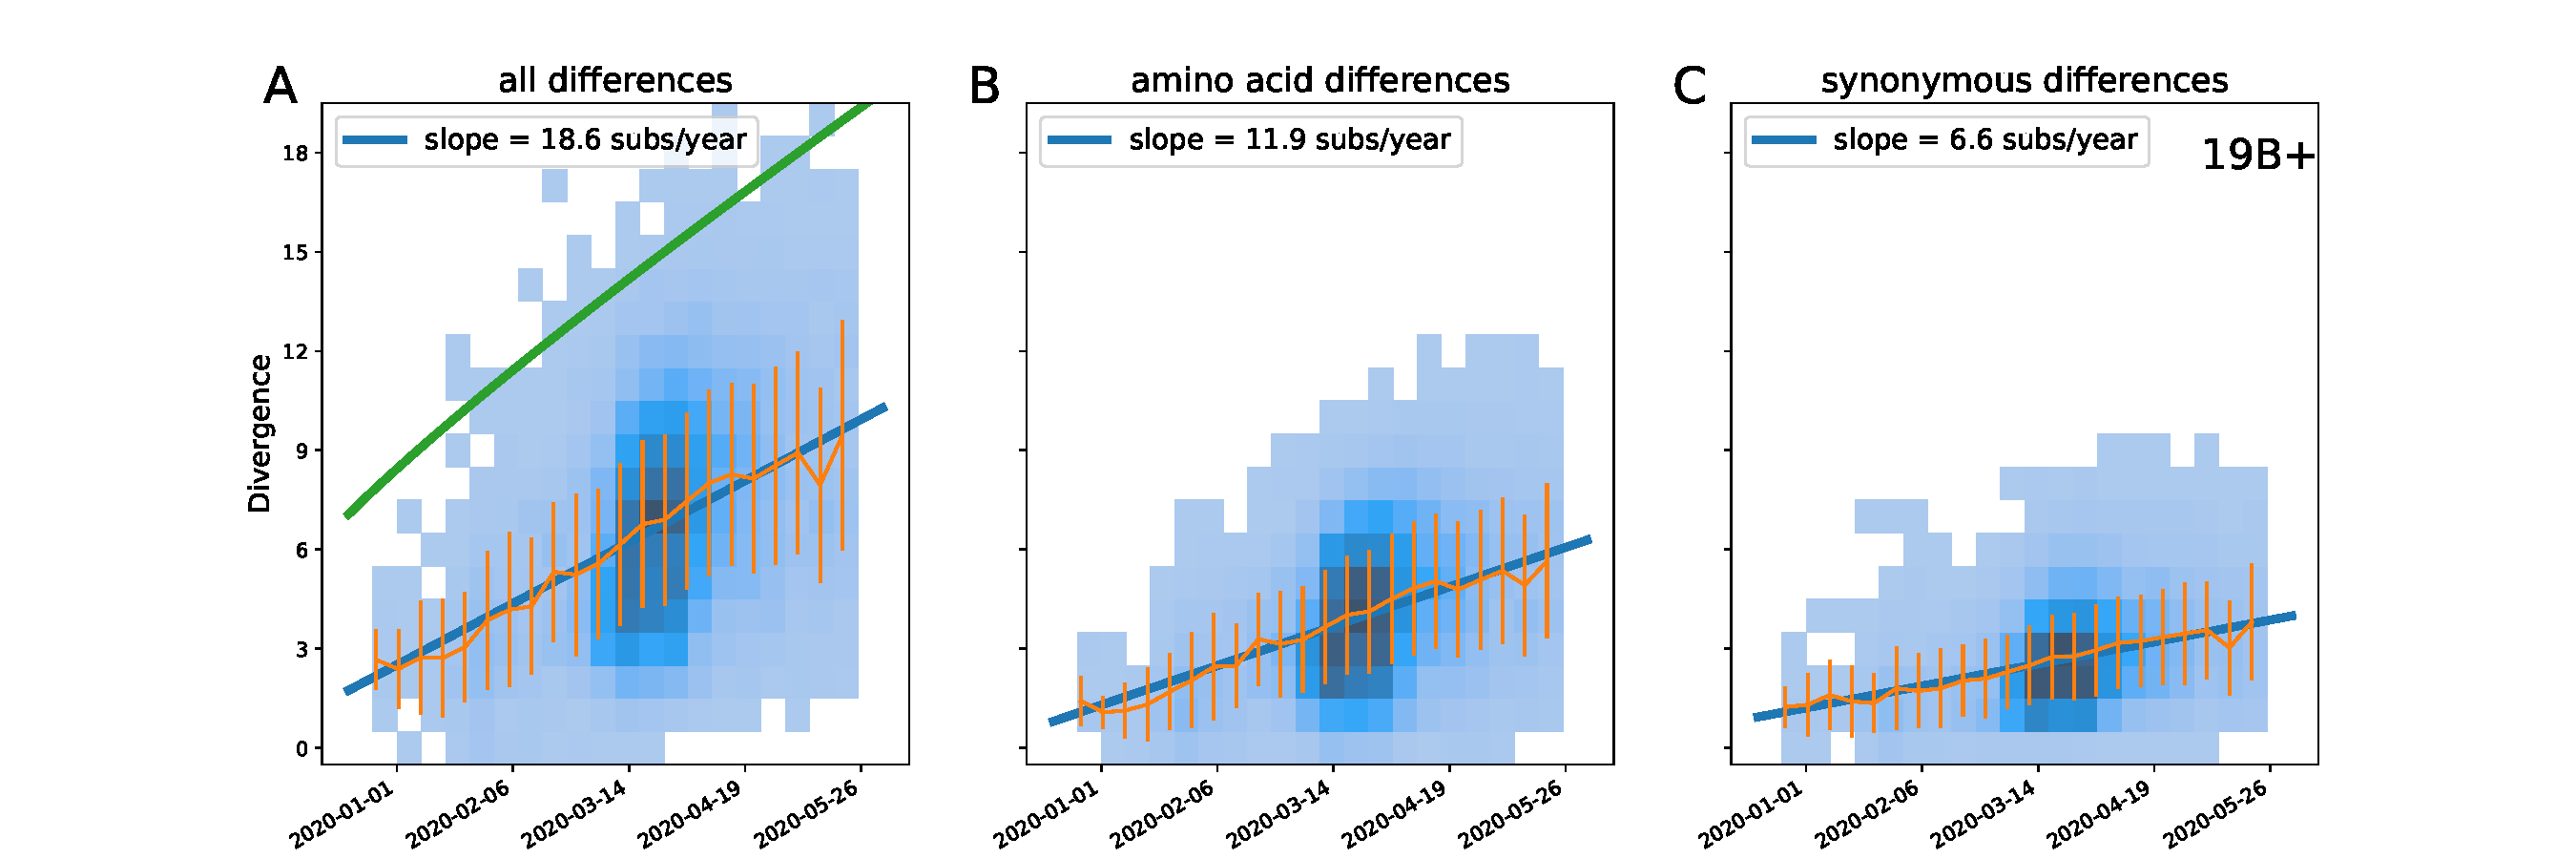
\includegraphics[width=0.8\textwidth]{figures/rtt/19B+_rtt.pdf}
    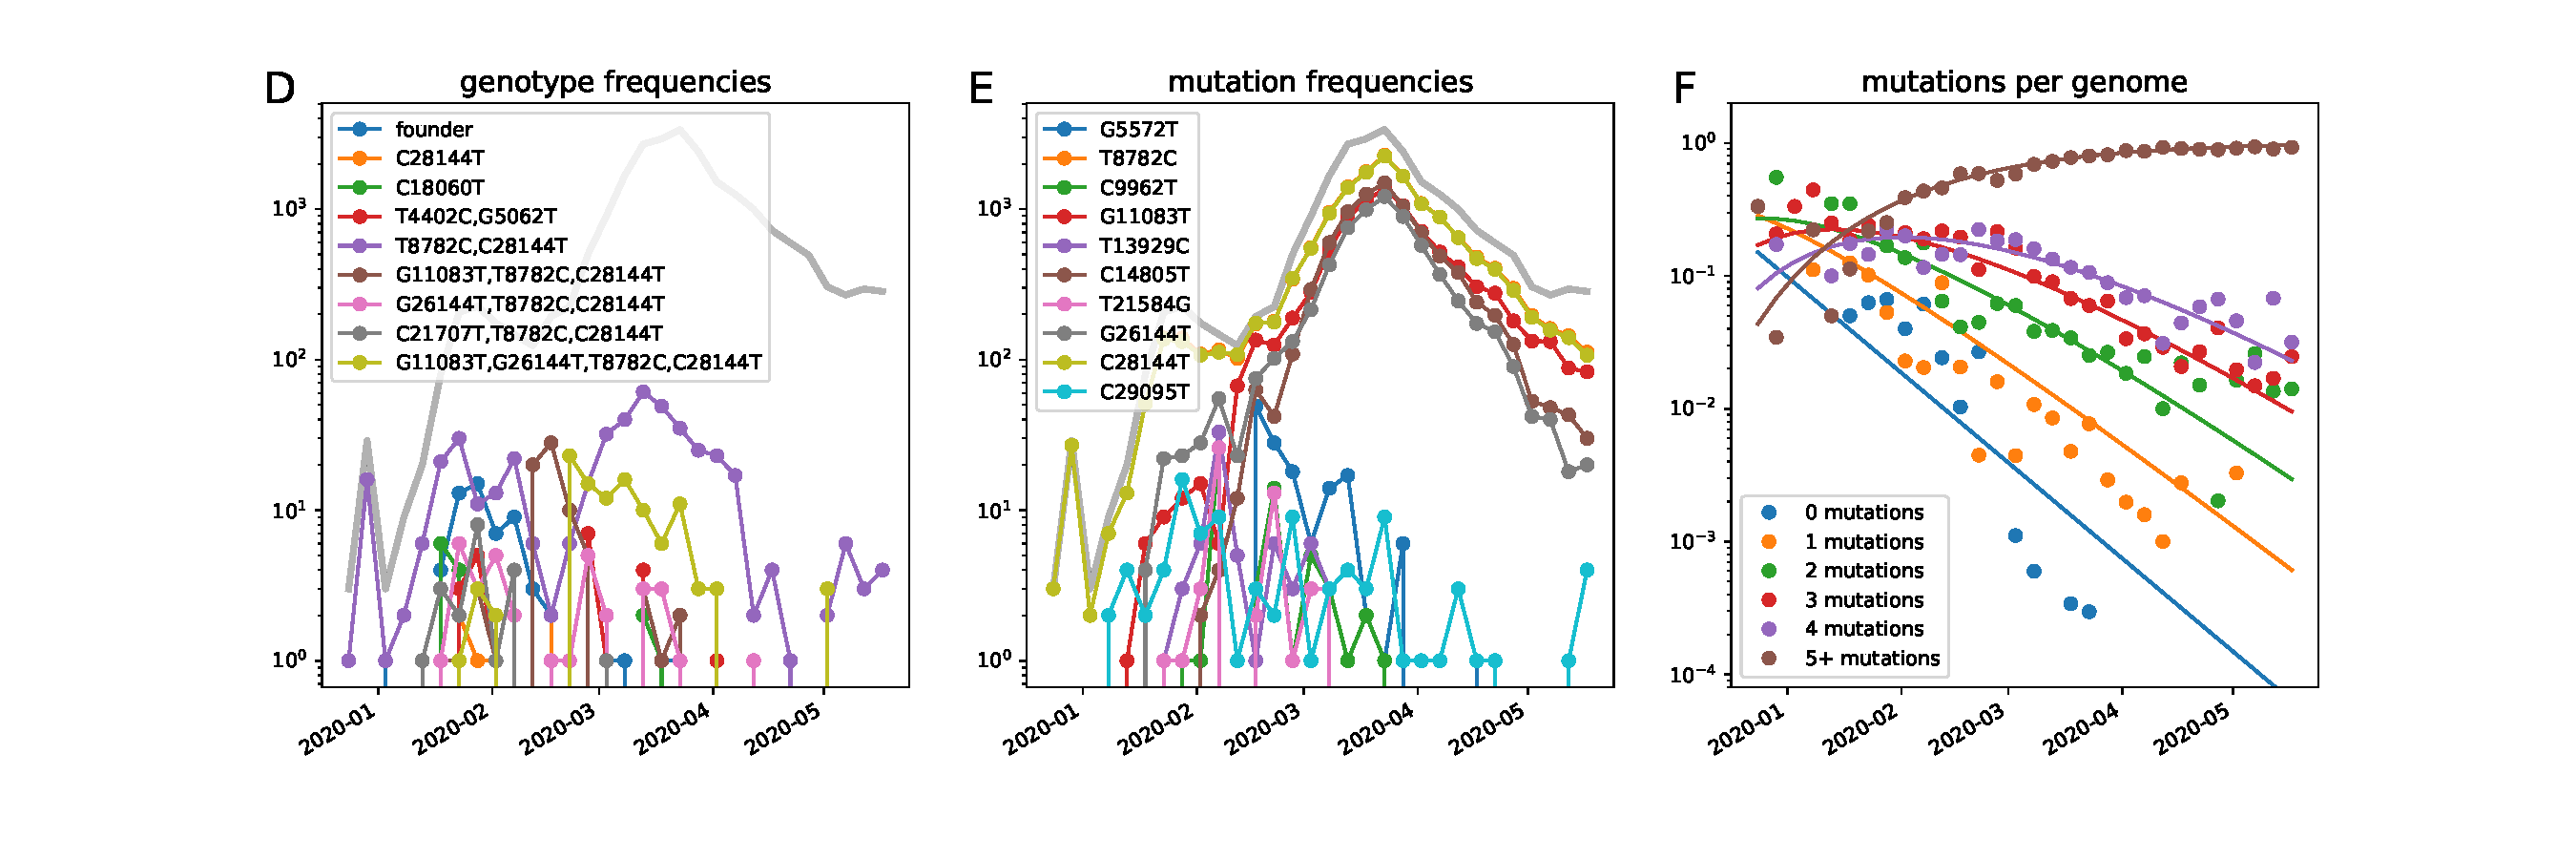
\includegraphics[width=0.8\textwidth]{figures/counts/19B+_counts.pdf}
    \caption{{\bf Divergence increases linearly with time in clade 19B+.}
    This figure contains sequences in clades 19 A and B rooted on clade 19B.
    \label{fig:19B+_divergence}}
\end{figure*}

\begin{figure*}[h]
    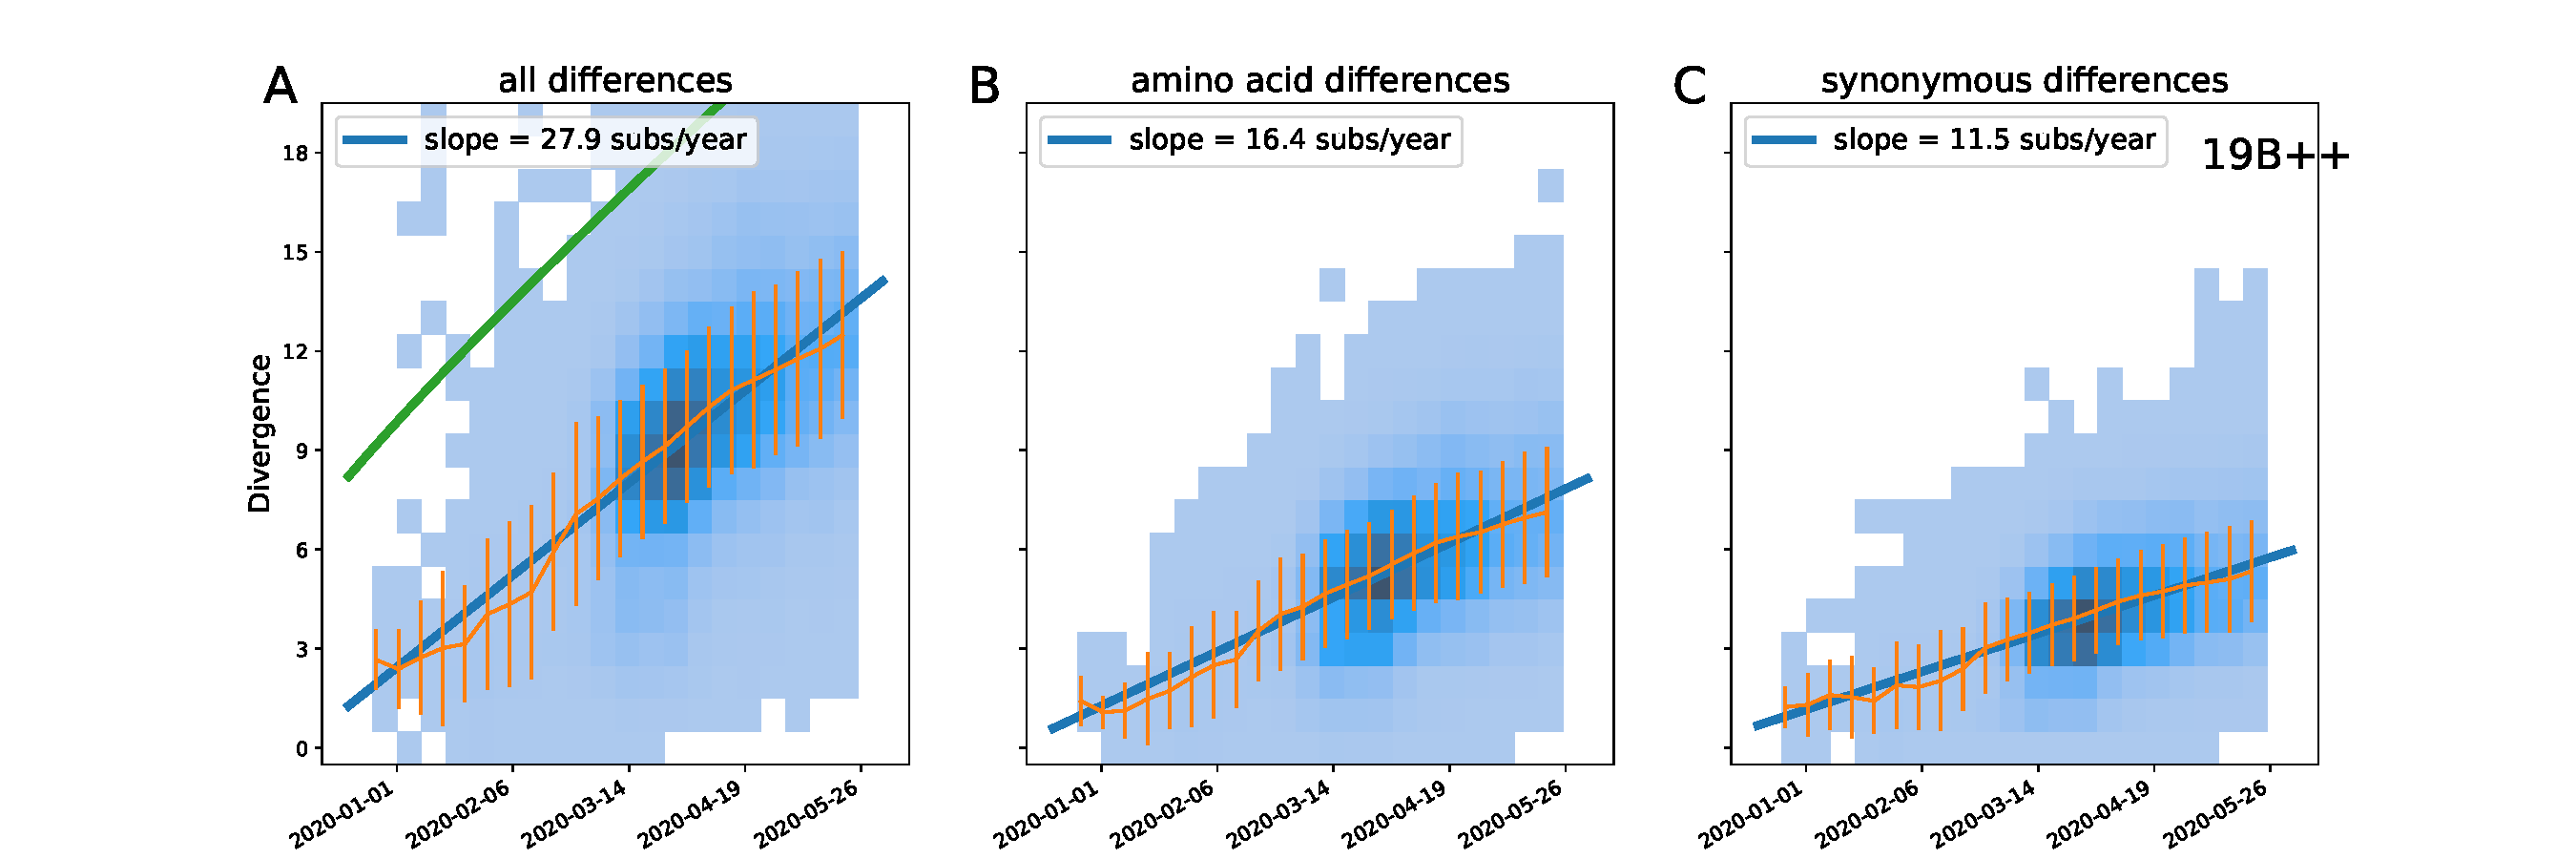
\includegraphics[width=0.8\textwidth]{figures/rtt/19B++_rtt.pdf}
    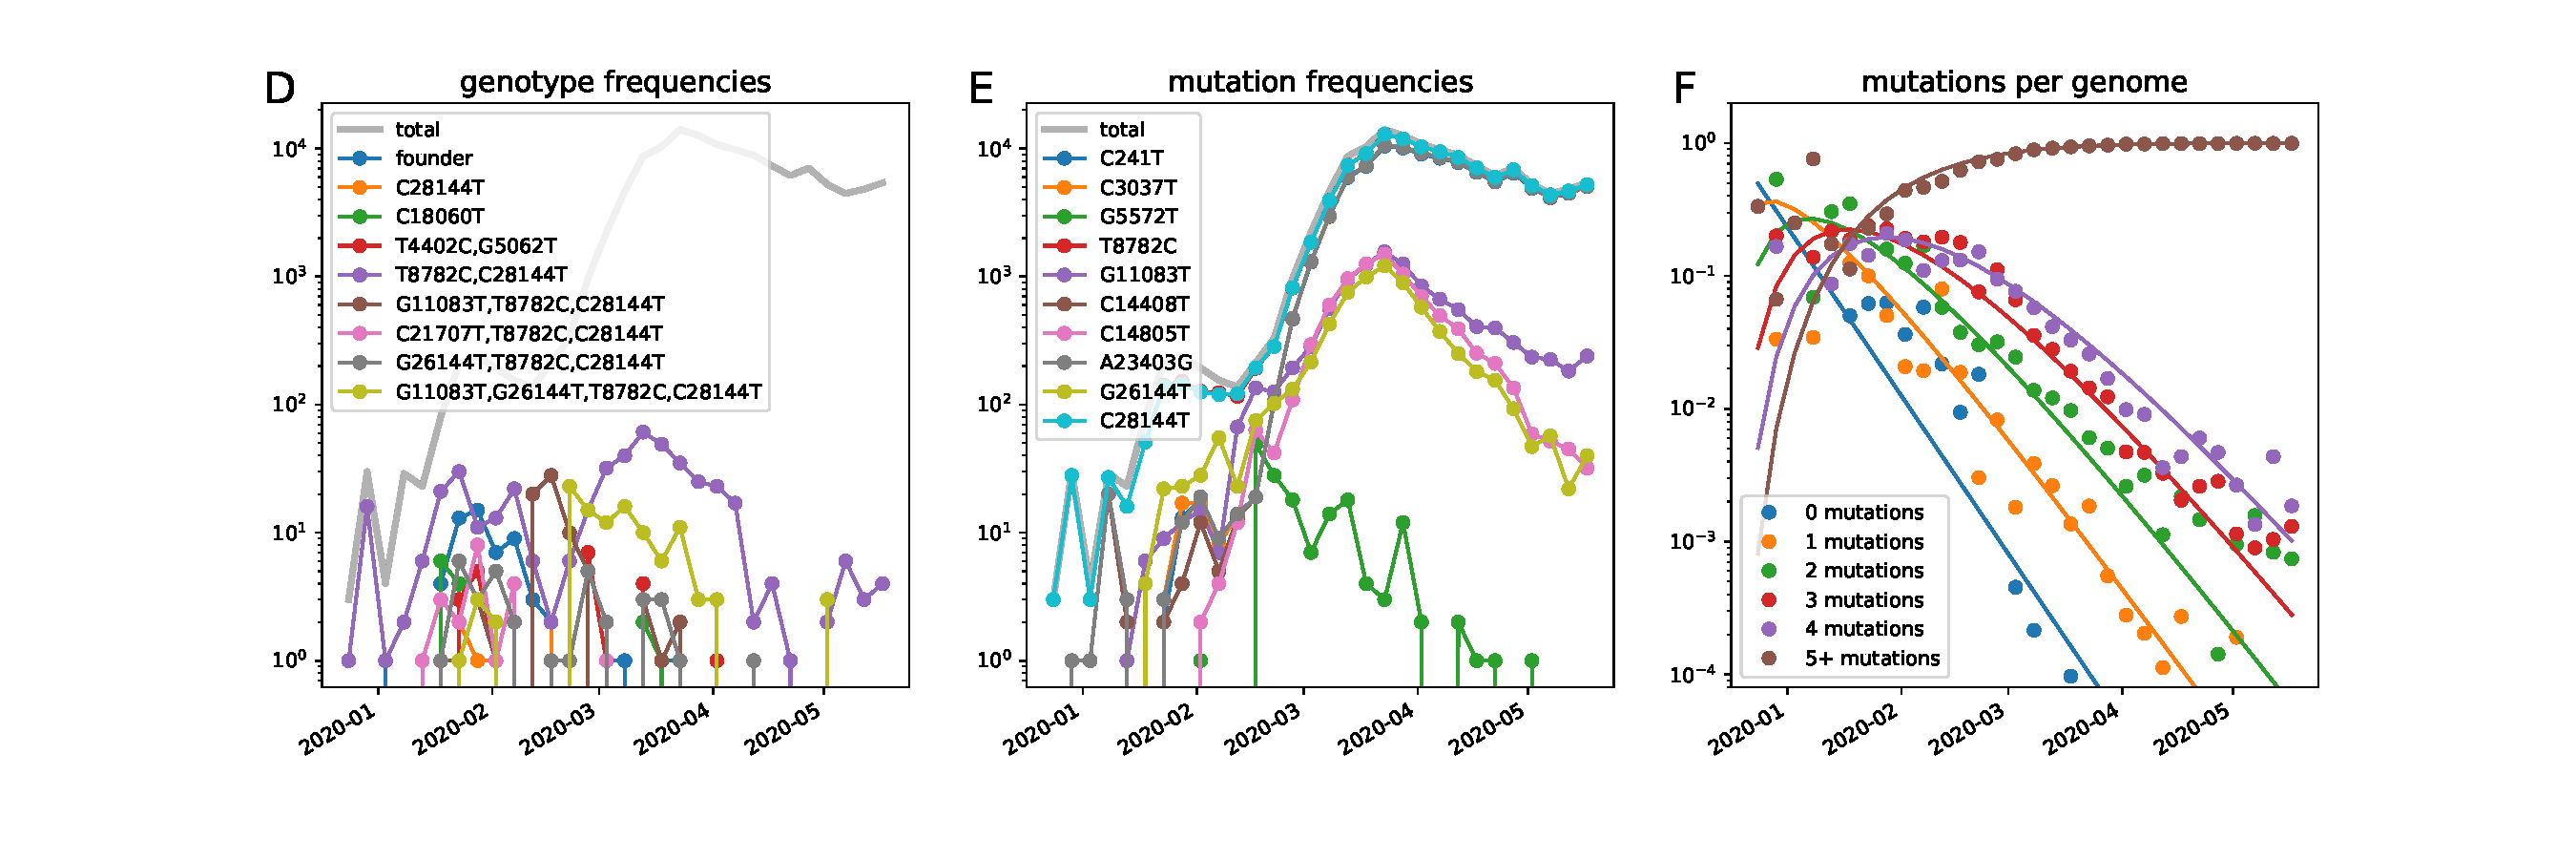
\includegraphics[width=0.8\textwidth]{figures/counts/19B++_counts.pdf}
    \caption{{\bf Divergence increases linearly with time in clade 19B++.}
    This figure contains sequences in clades 19A, 19B, 20A, 20B, 20C, and 20D rooted on clade 19B.
    \label{fig:19B++_divergence}}
\end{figure*}

\begin{figure*}[h]
    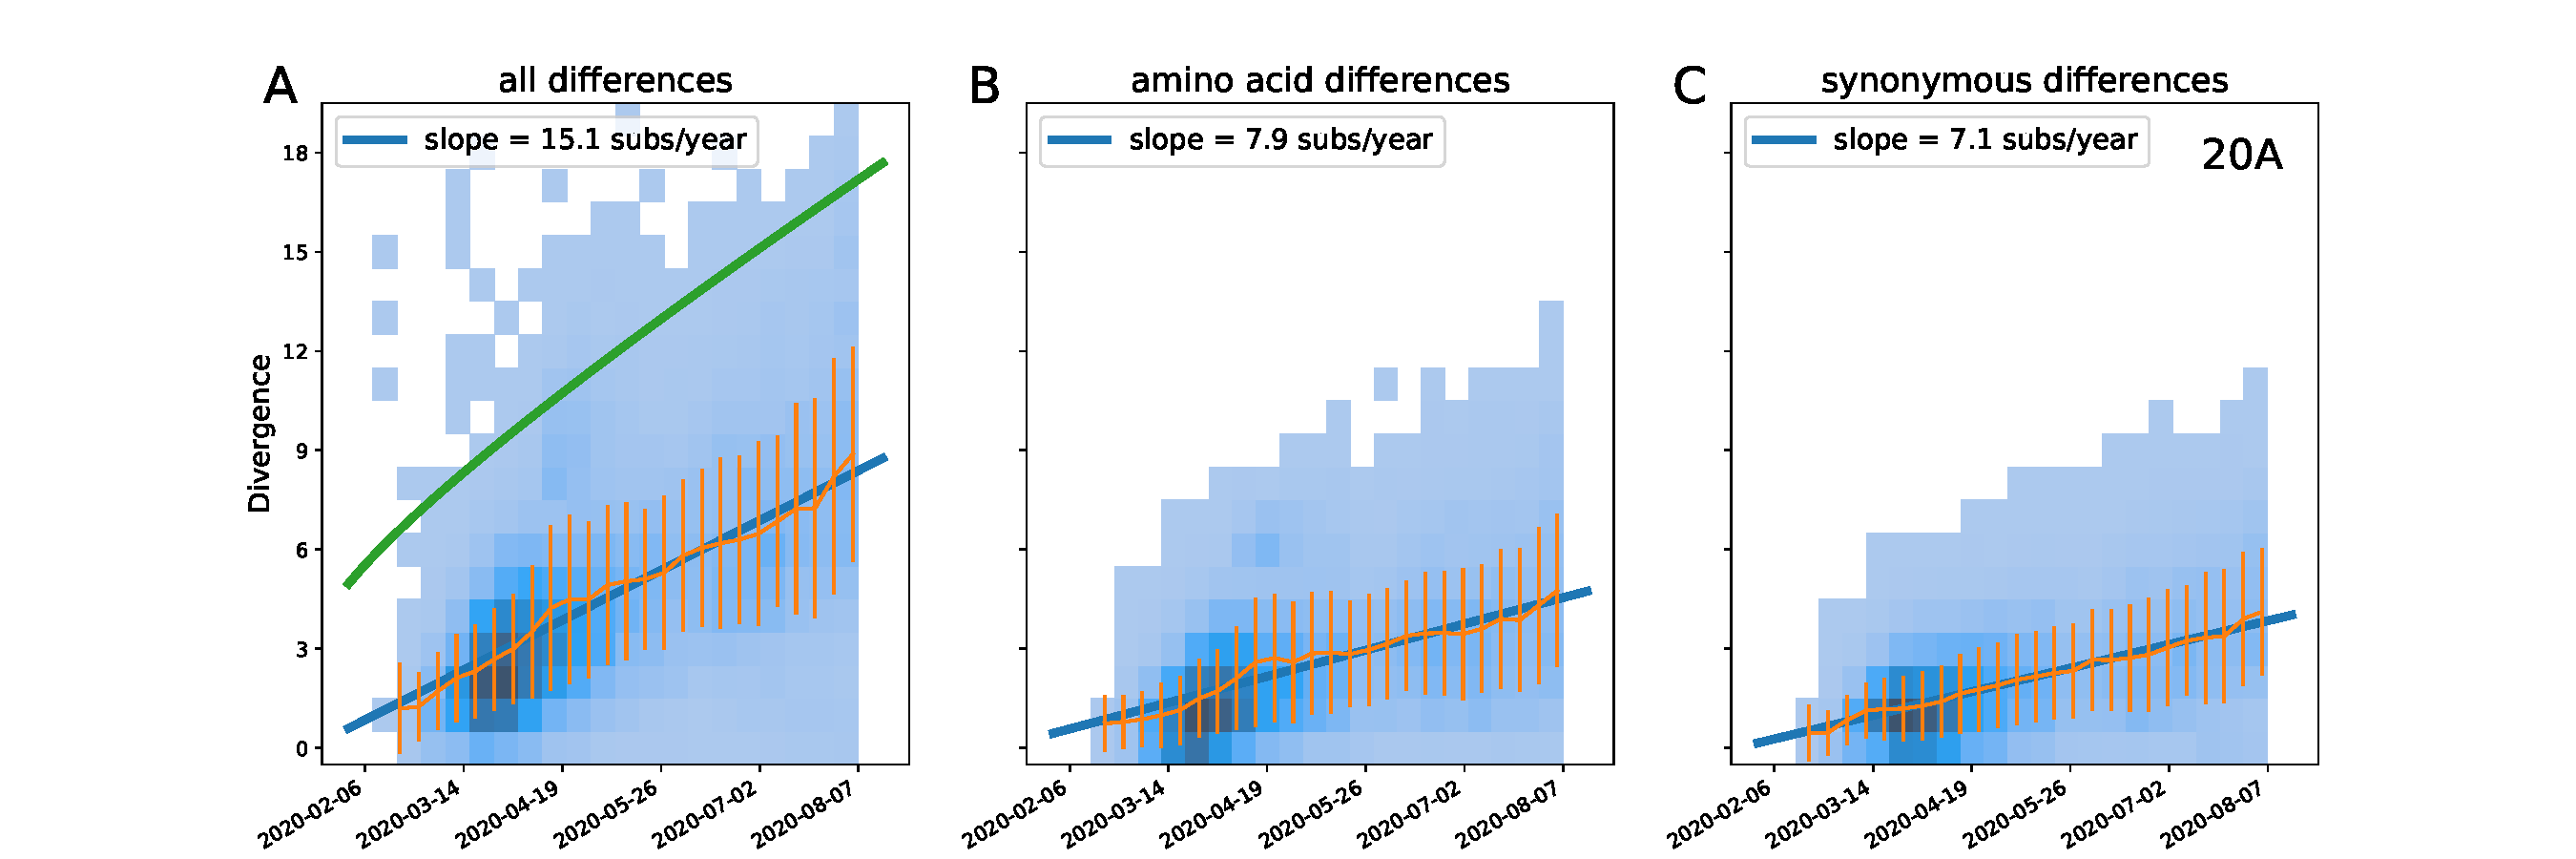
\includegraphics[width=0.8\textwidth]{figures/rtt/20A_rtt.pdf}
    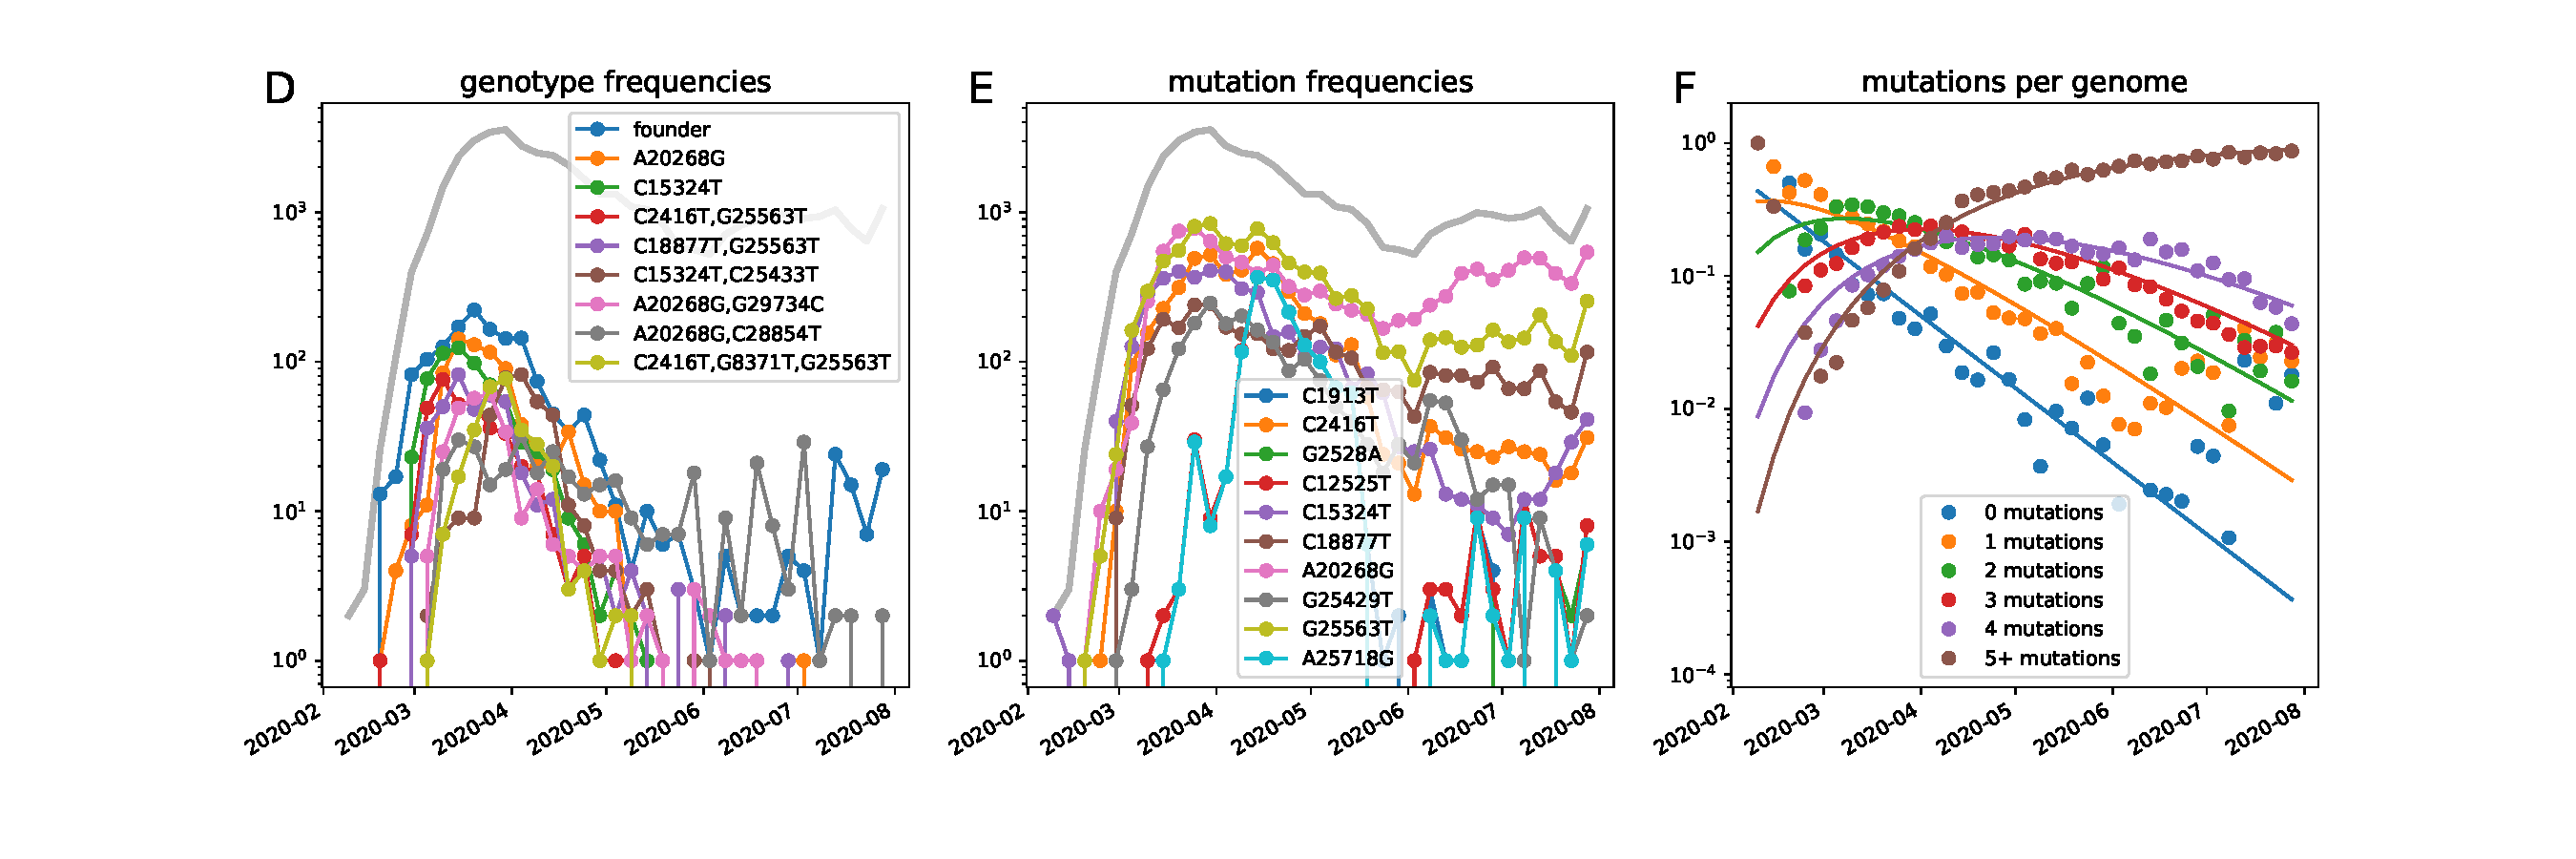
\includegraphics[width=0.8\textwidth]{figures/counts/20A_counts.pdf}
    \caption{{\bf Divergence increases linearly with time in clade 20A.}
    \label{fig:20A_divergence}}
\end{figure*}

\begin{figure*}[h]
    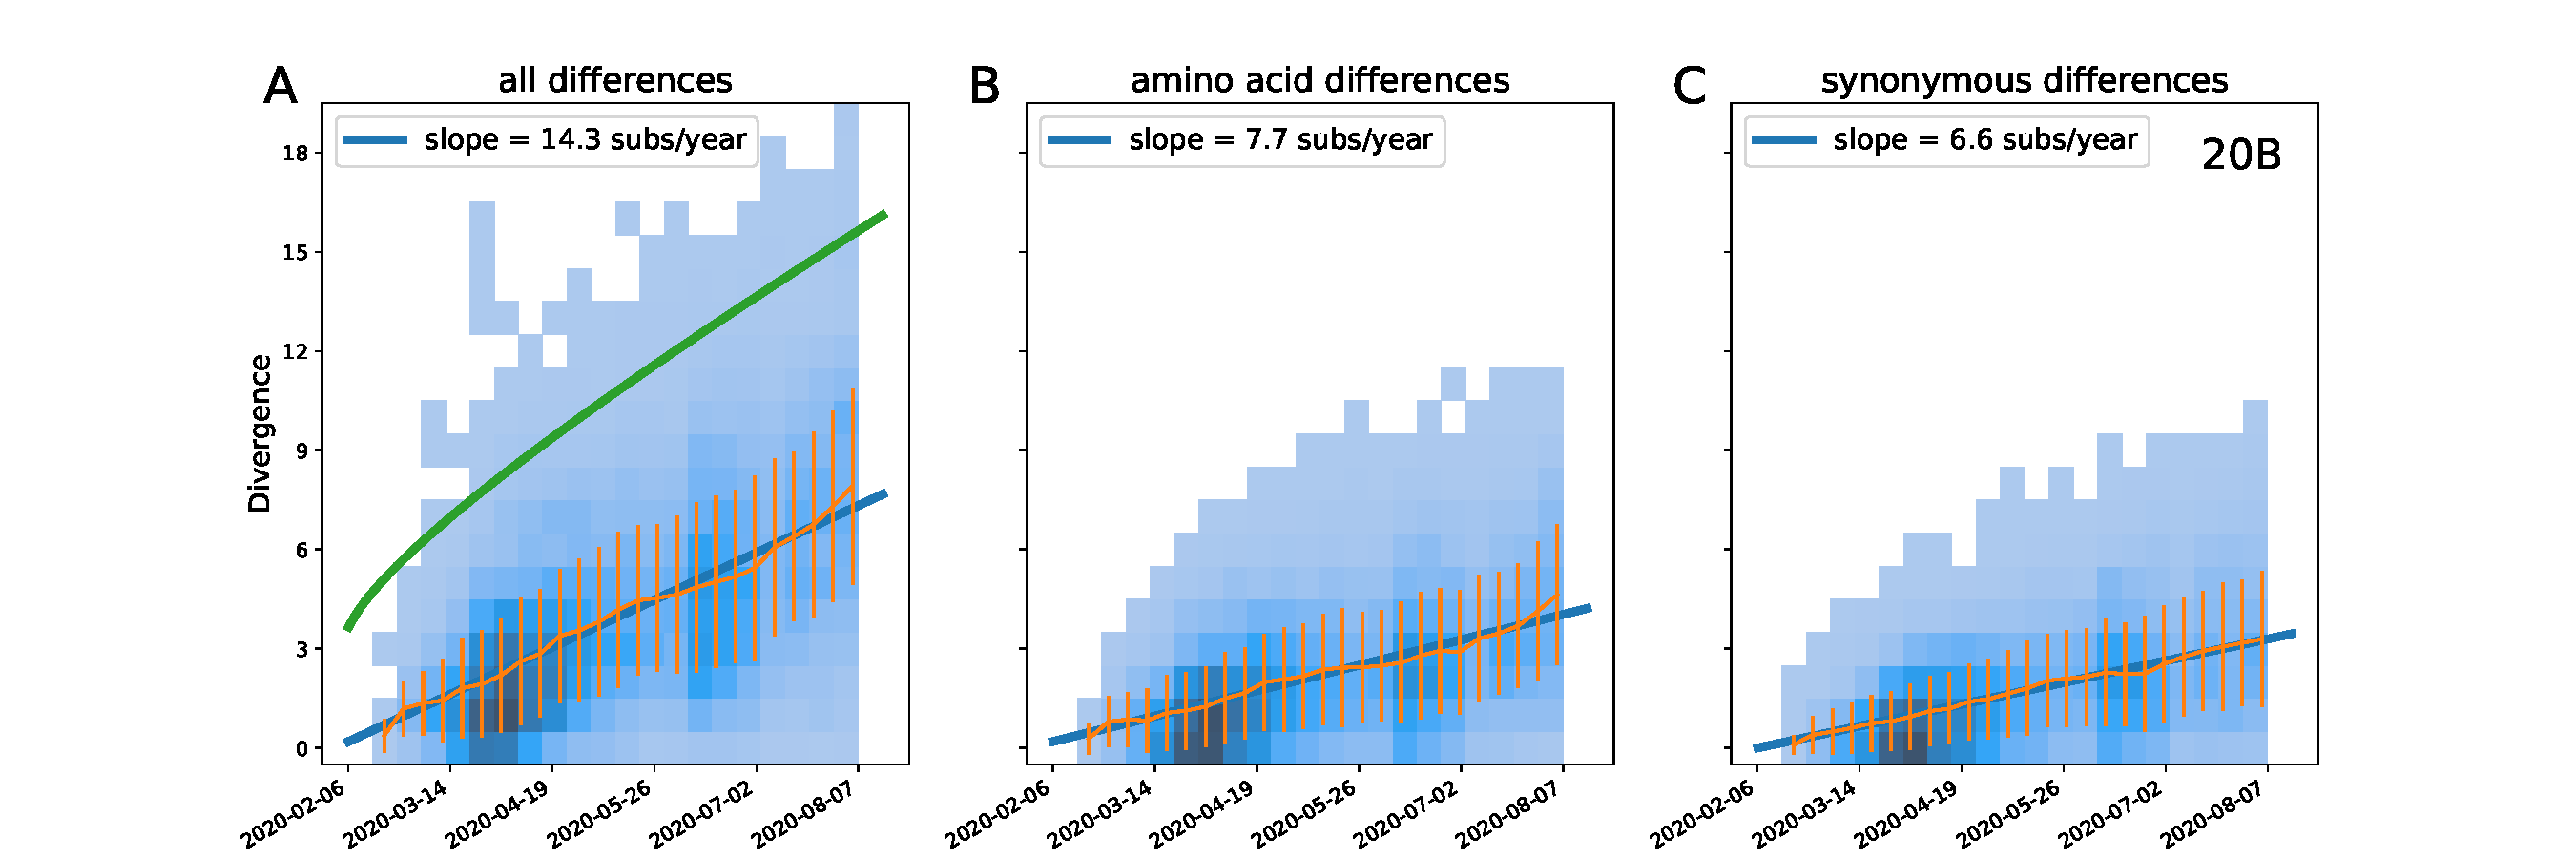
\includegraphics[width=0.8\textwidth]{figures/rtt/20B_rtt.pdf}
    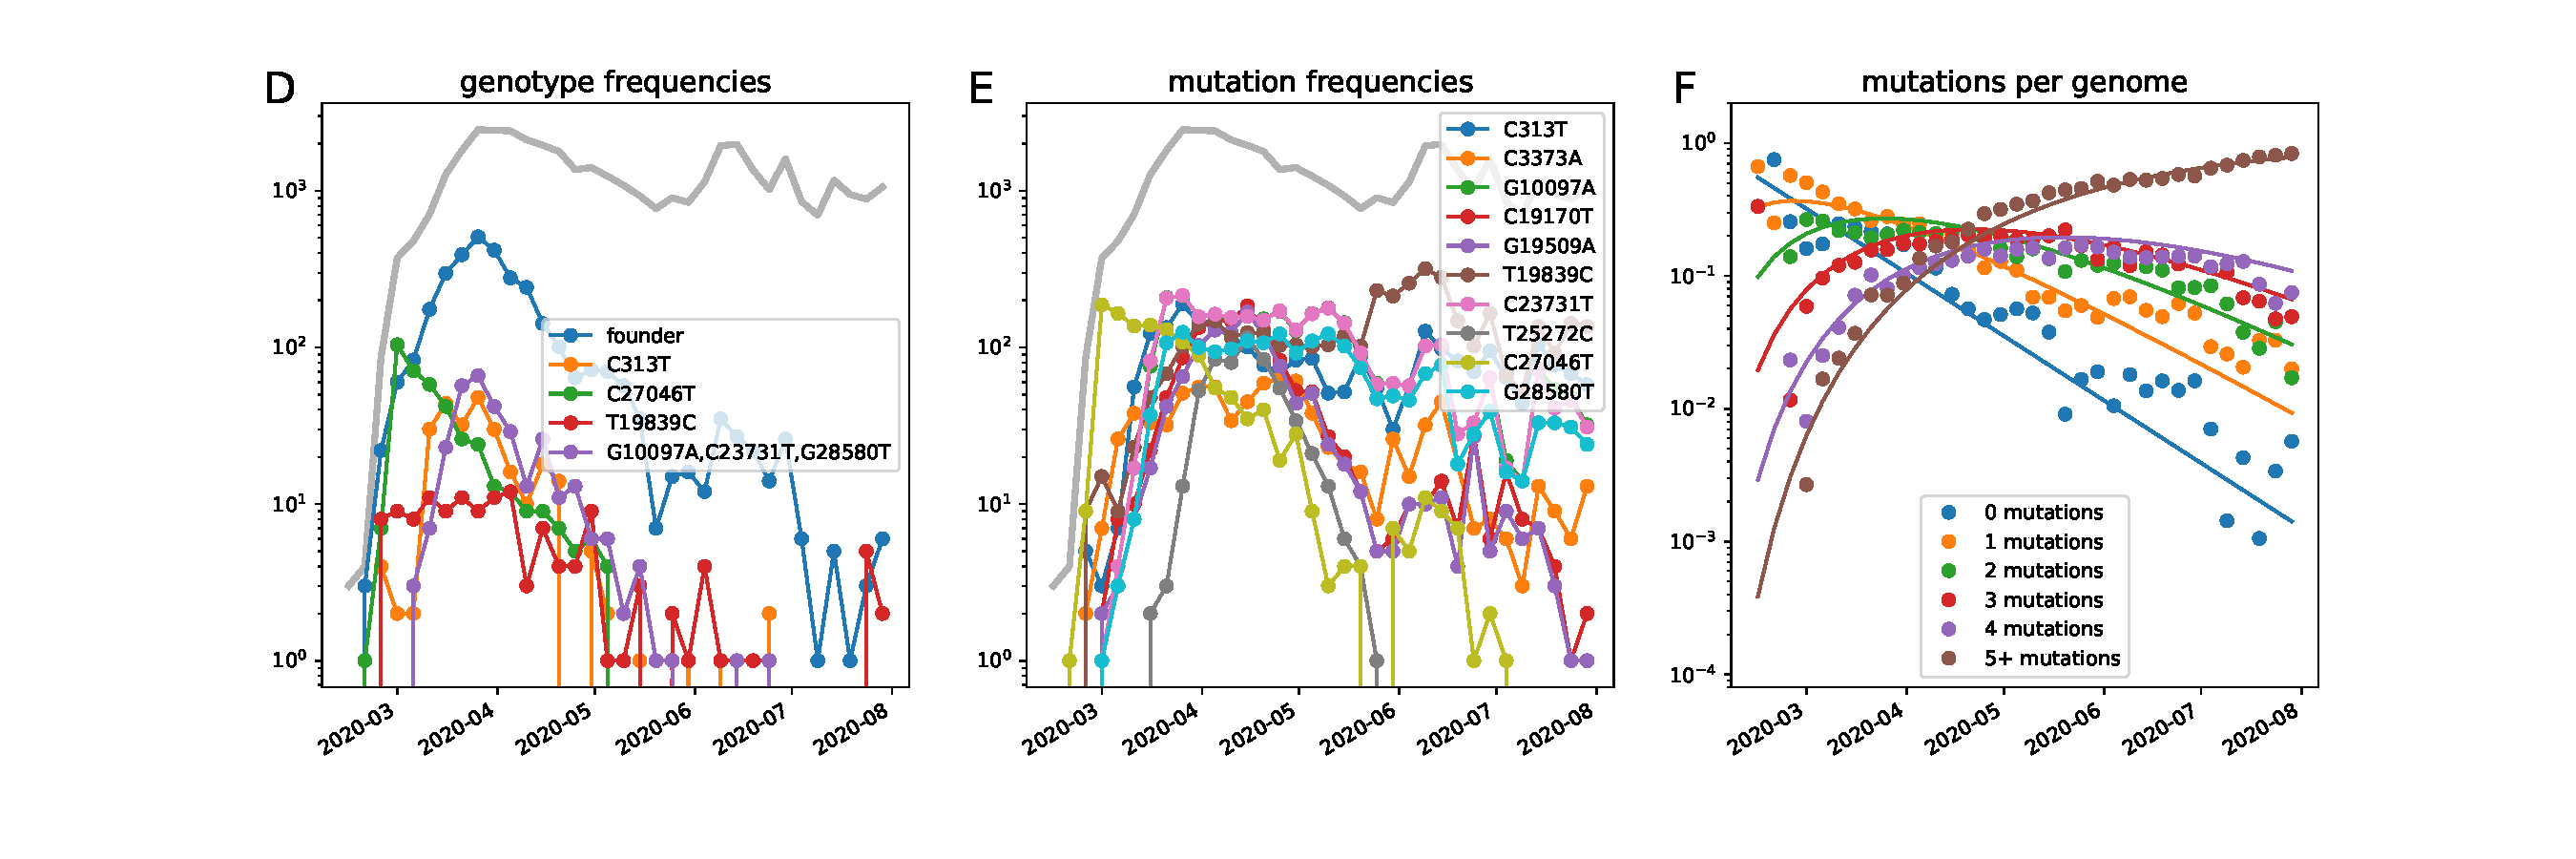
\includegraphics[width=0.8\textwidth]{figures/counts/20B_counts.pdf}
    \caption{{\bf Divergence increases linearly with time in clade 20B.}
    \label{fig:20B_divergence}}
\end{figure*}

\begin{figure*}[h]
    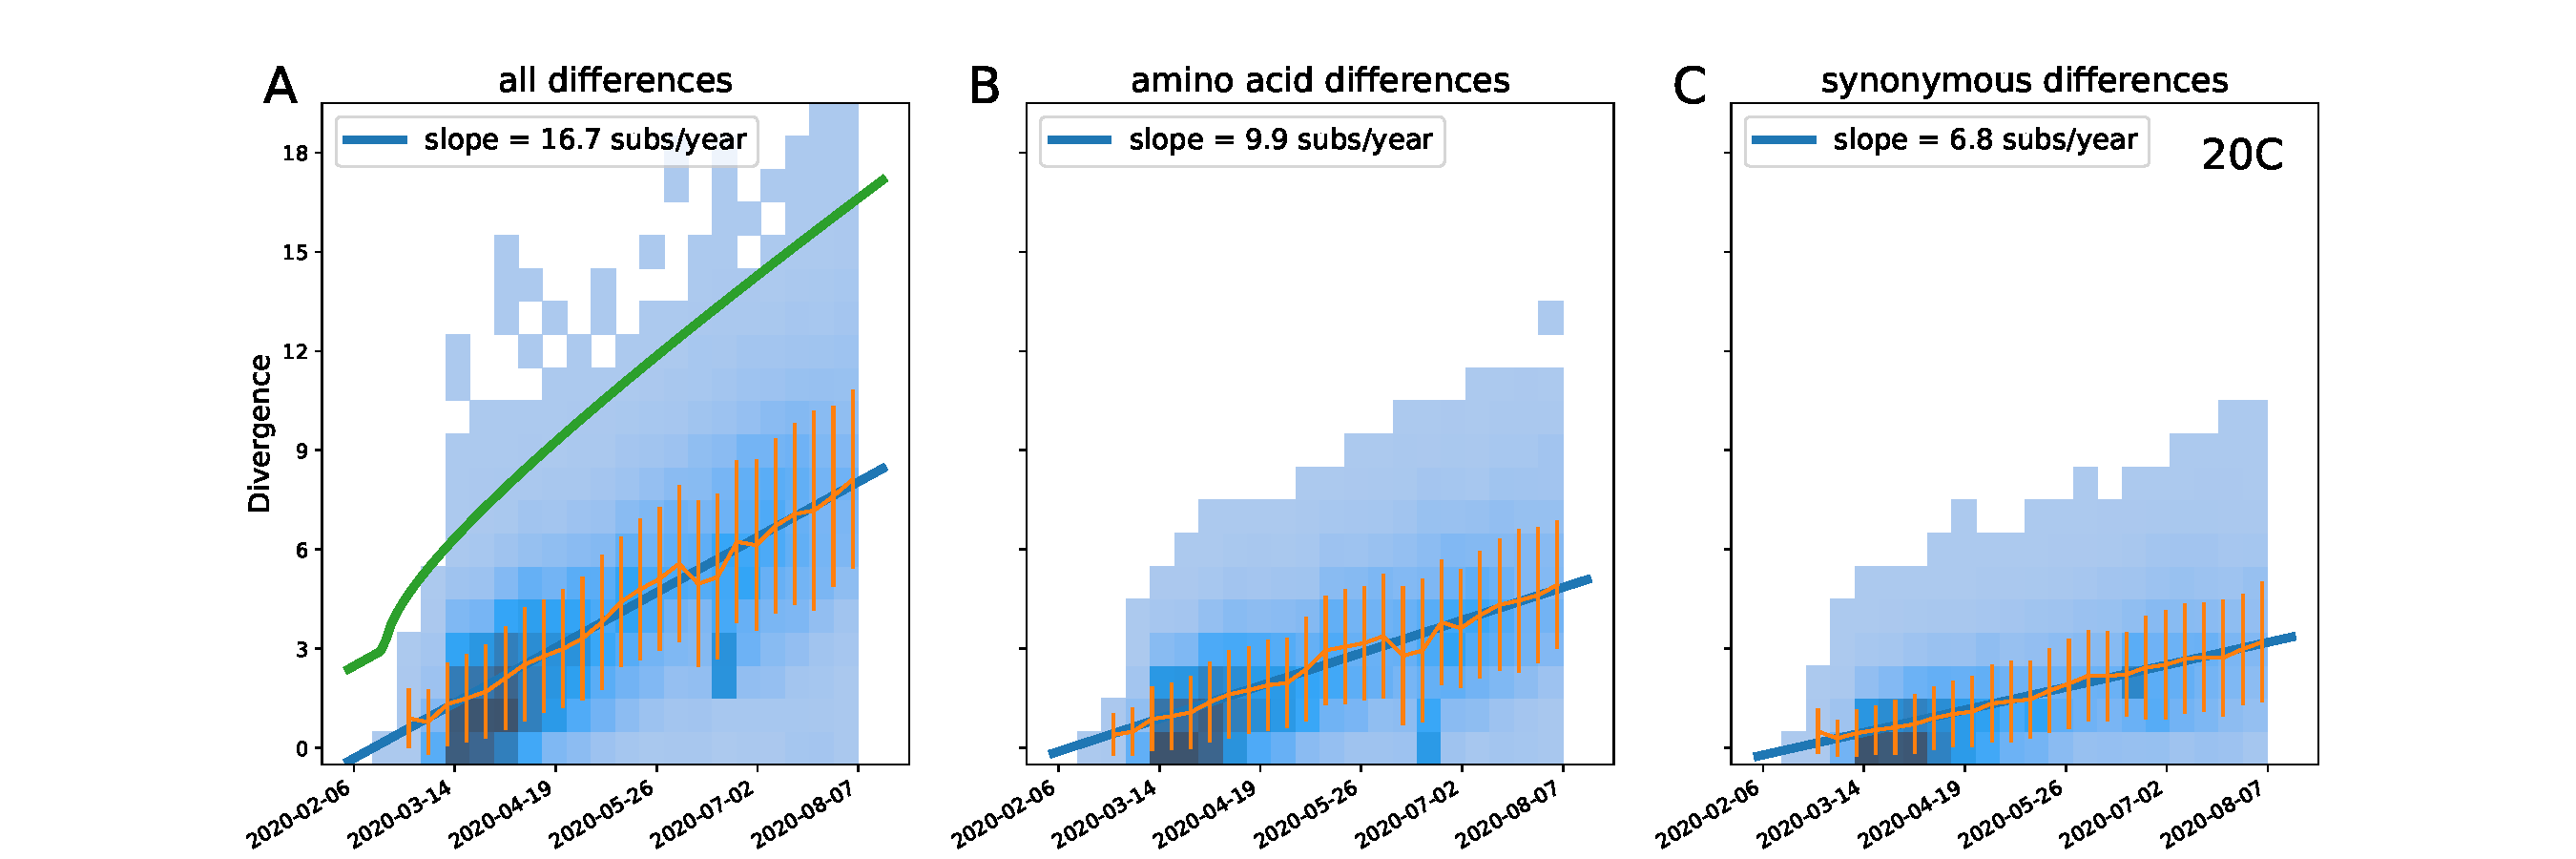
\includegraphics[width=0.8\textwidth]{figures/rtt/20C_rtt.pdf}
    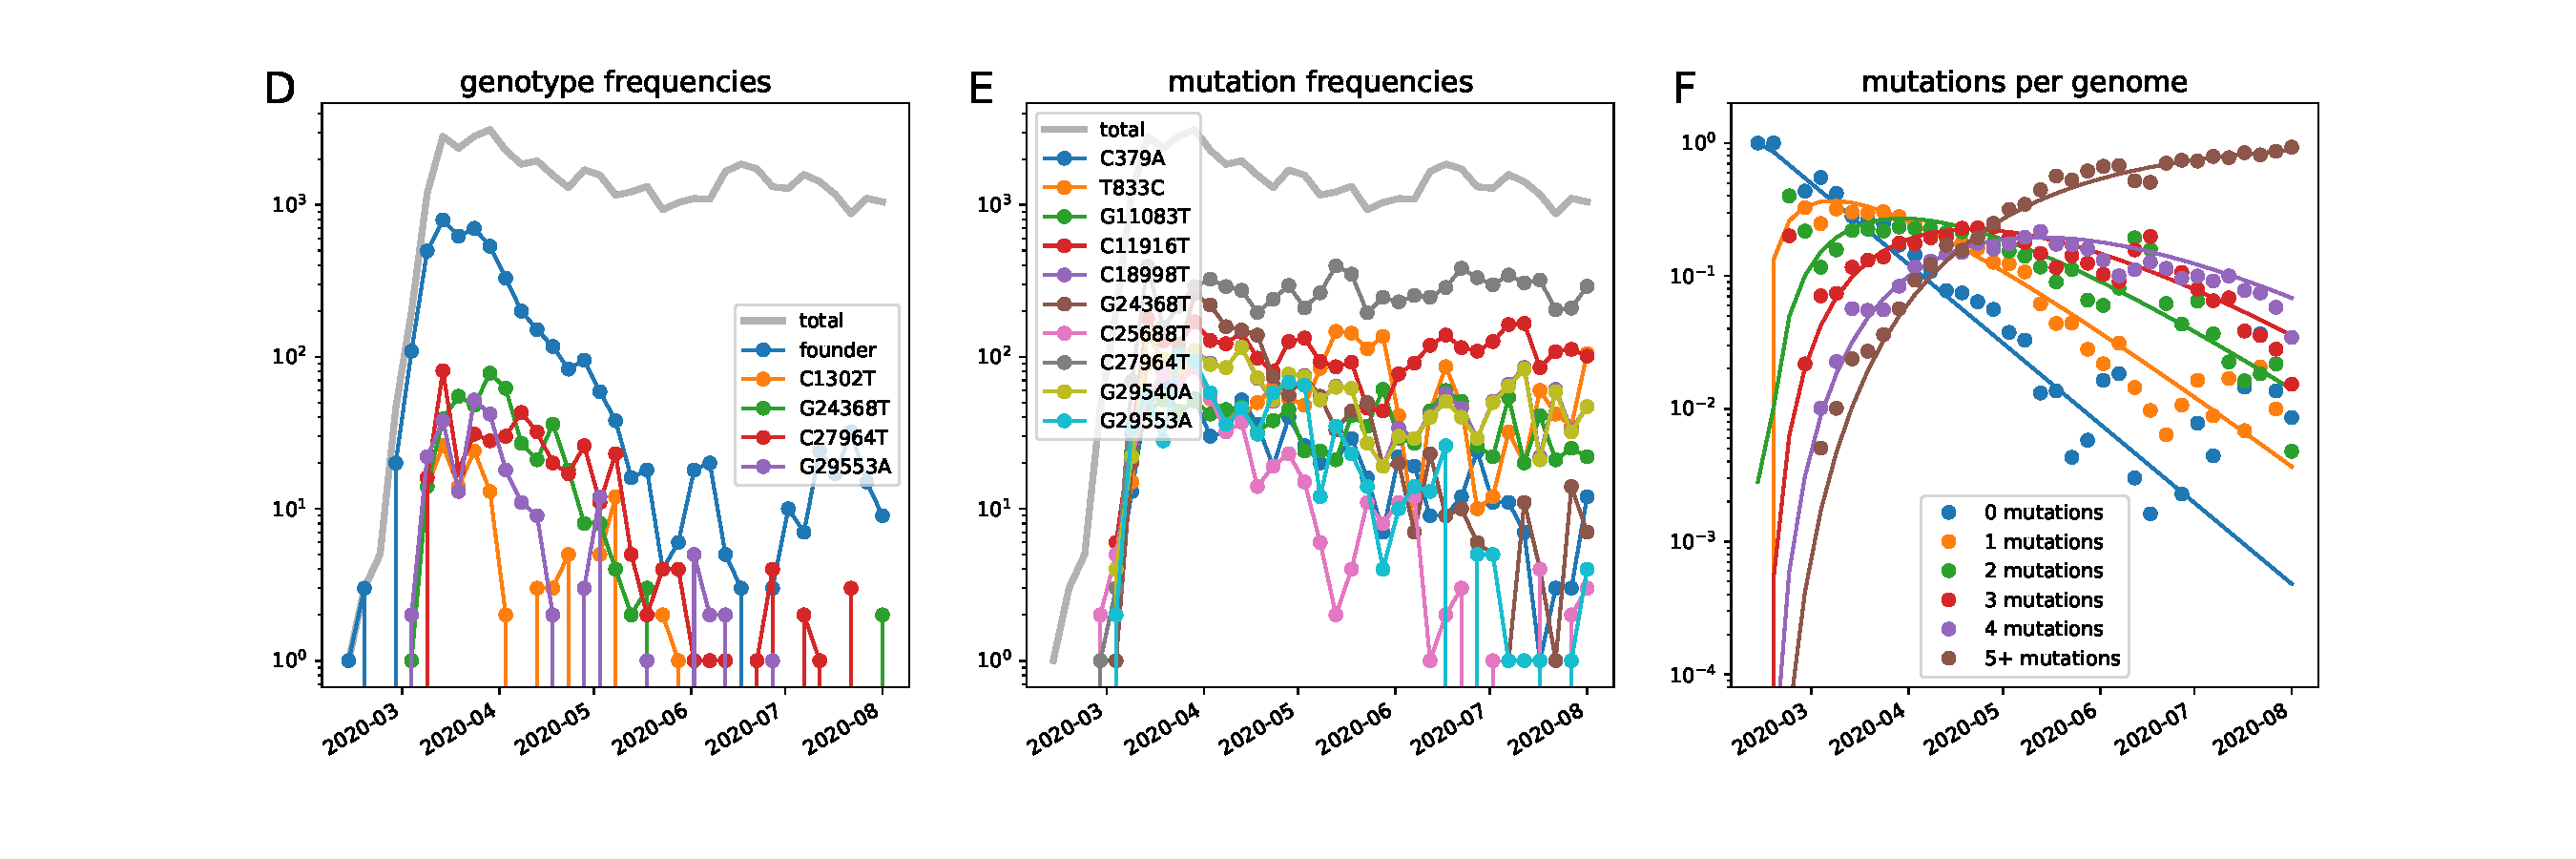
\includegraphics[width=0.8\textwidth]{figures/counts/20C_counts.pdf}
    \caption{{\bf Divergence increases linearly with time in clade 20C.}
    \label{fig:20C_divergence}}
\end{figure*}


\begin{figure*}[h]
    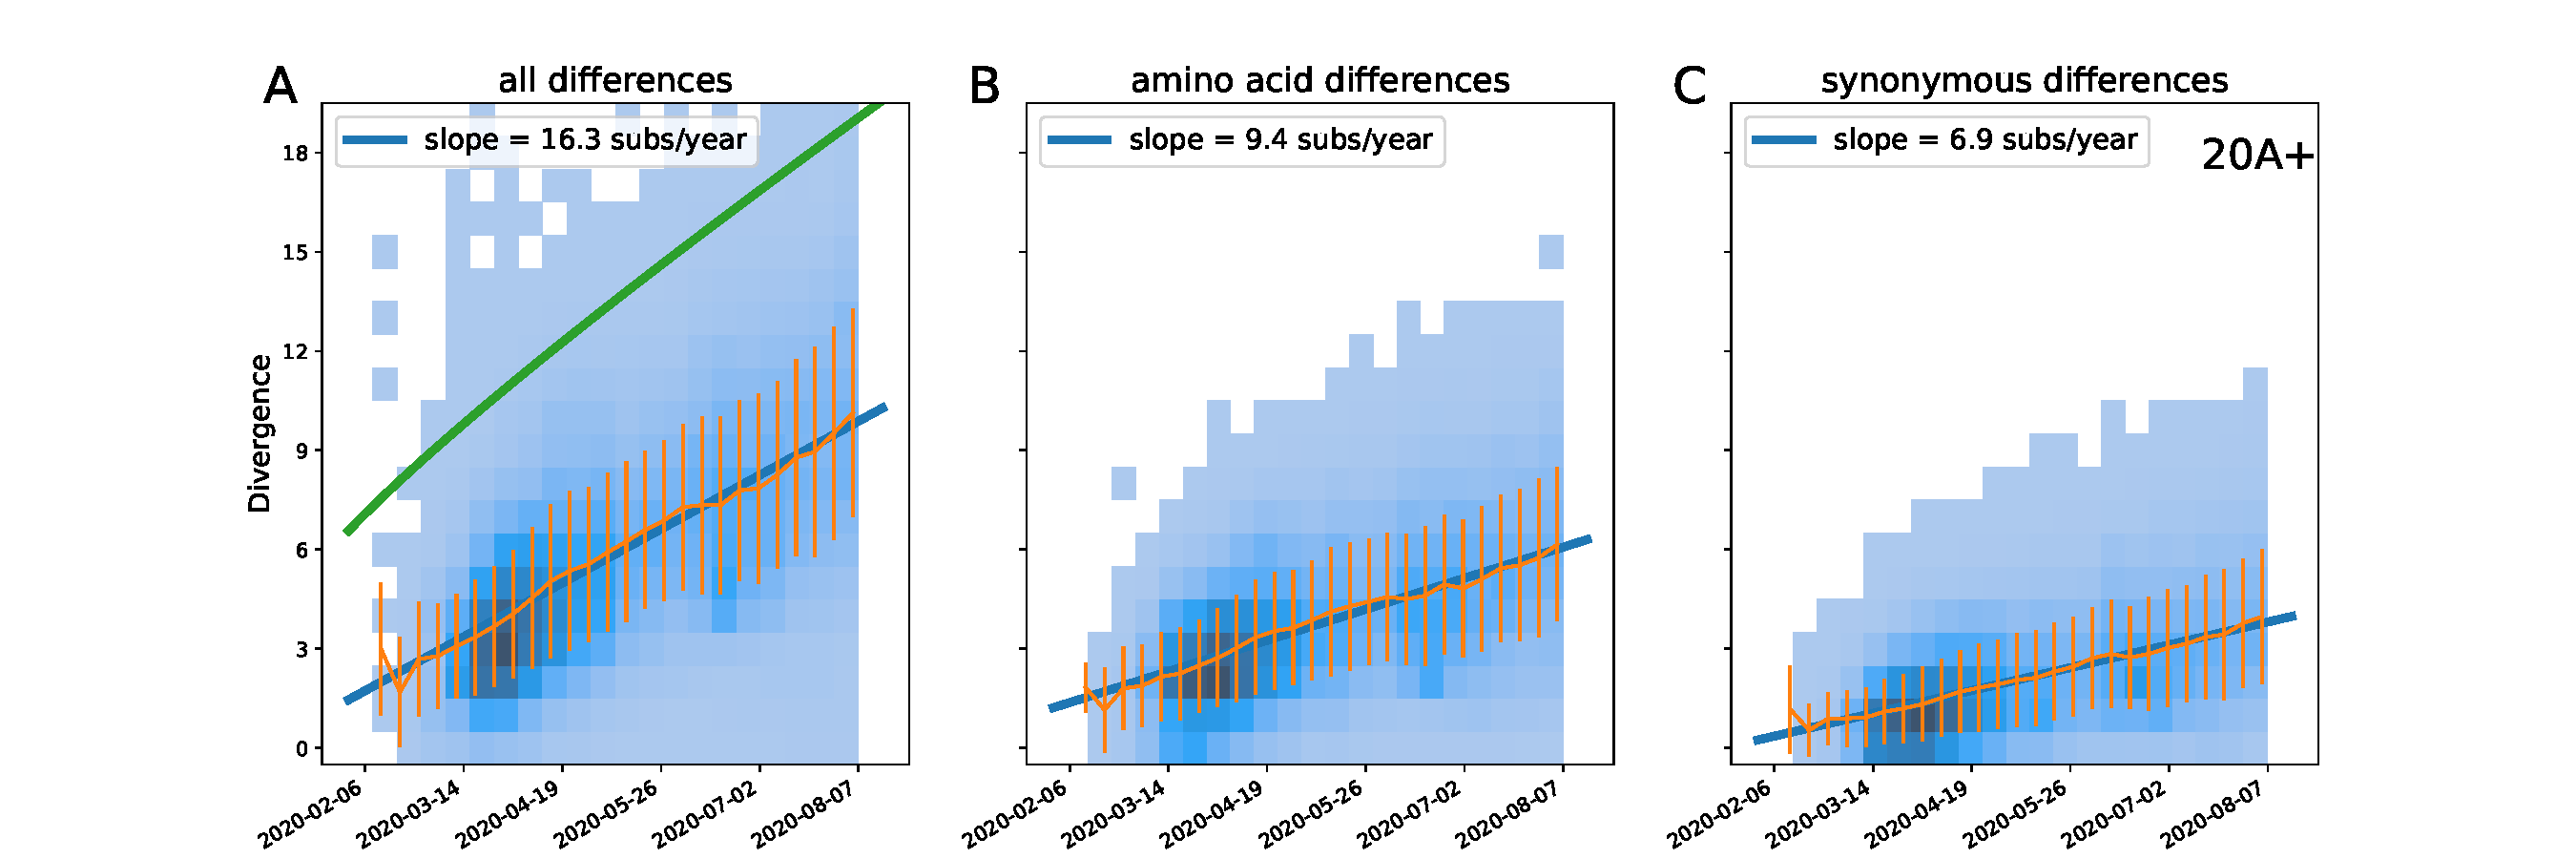
\includegraphics[width=0.8\textwidth]{figures/rtt/20A+_rtt.pdf}
    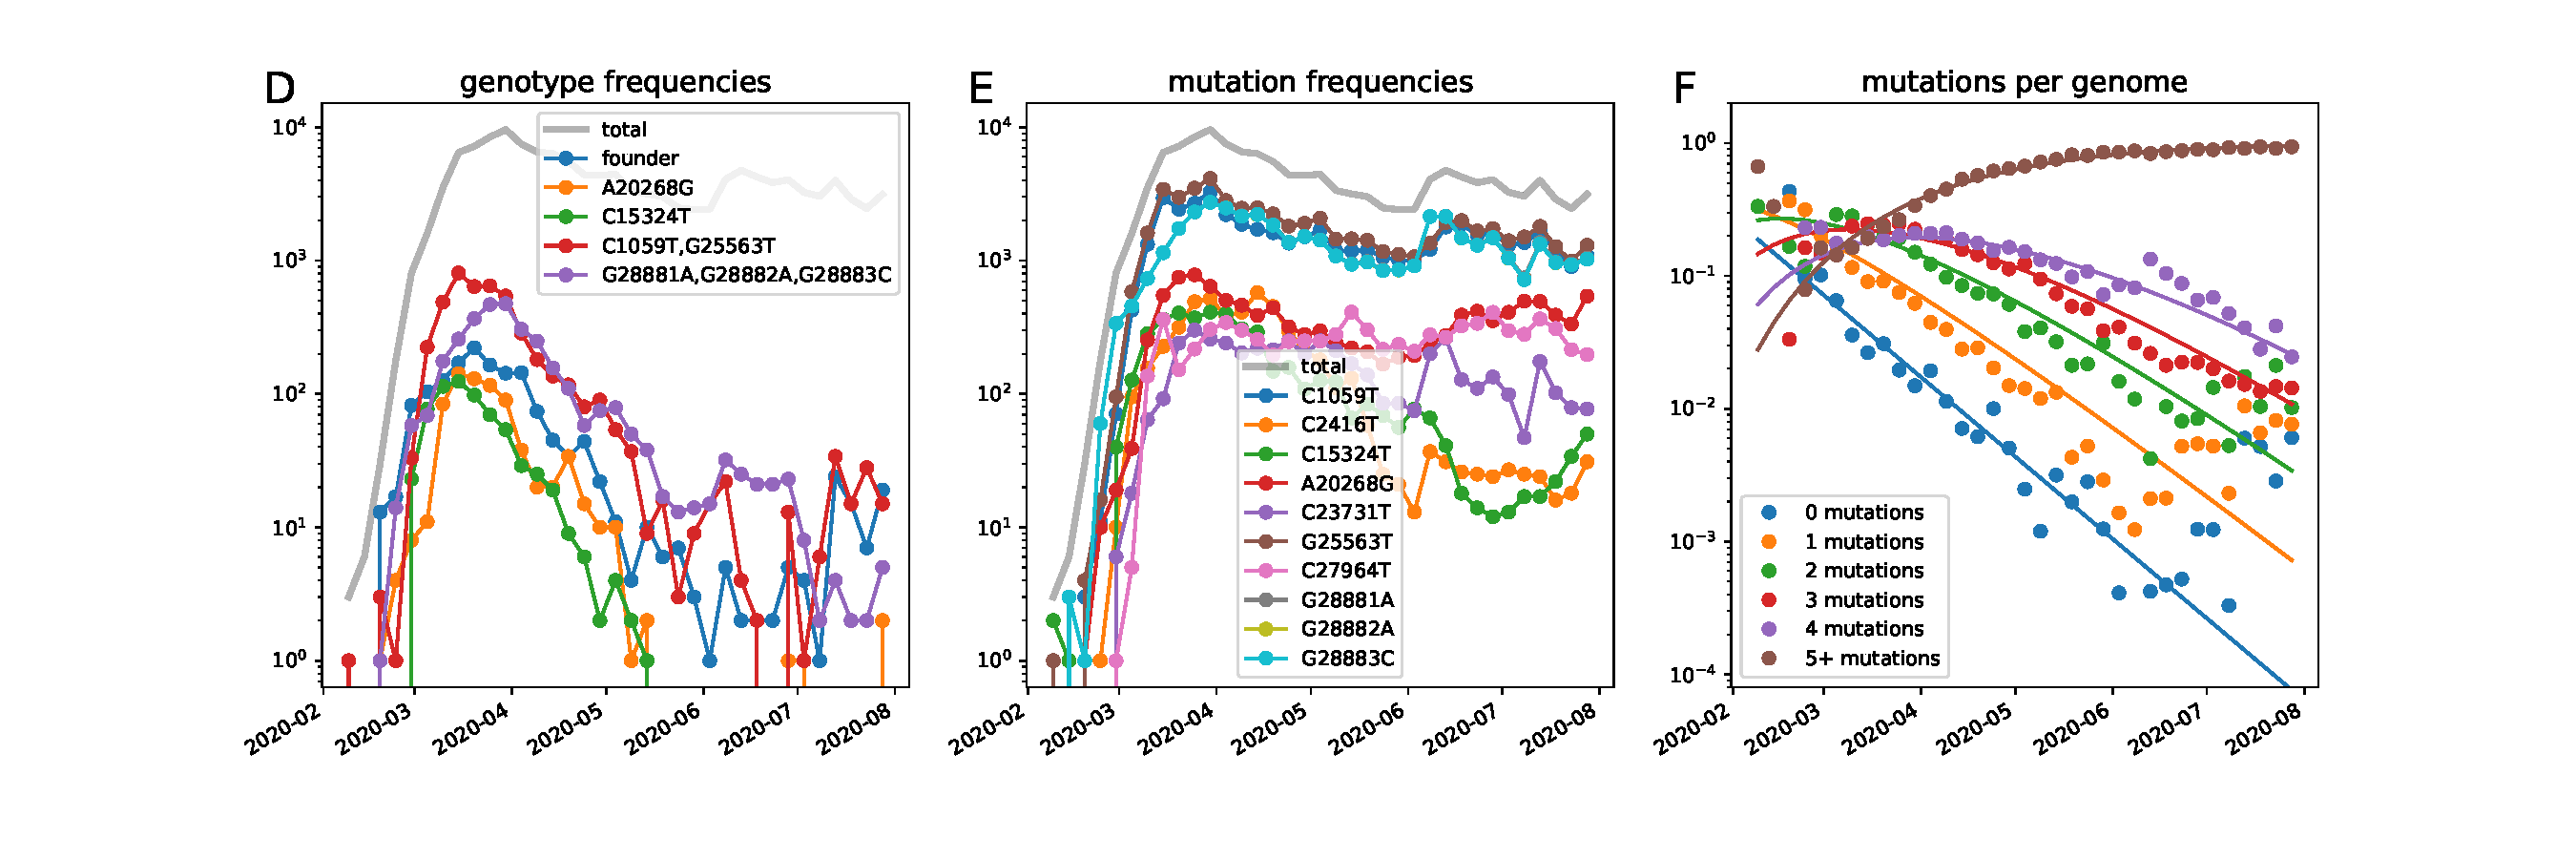
\includegraphics[width=0.8\textwidth]{figures/counts/20A+_counts.pdf}
    \caption{{\bf Divergence increases linearly with time in clade 20A+.}
    This figure contains sequences in clades 20A,B,C,D rooted on clade 20A.
    \label{fig:20A+_divergence}}
\end{figure*}



\begin{figure*}[h]
    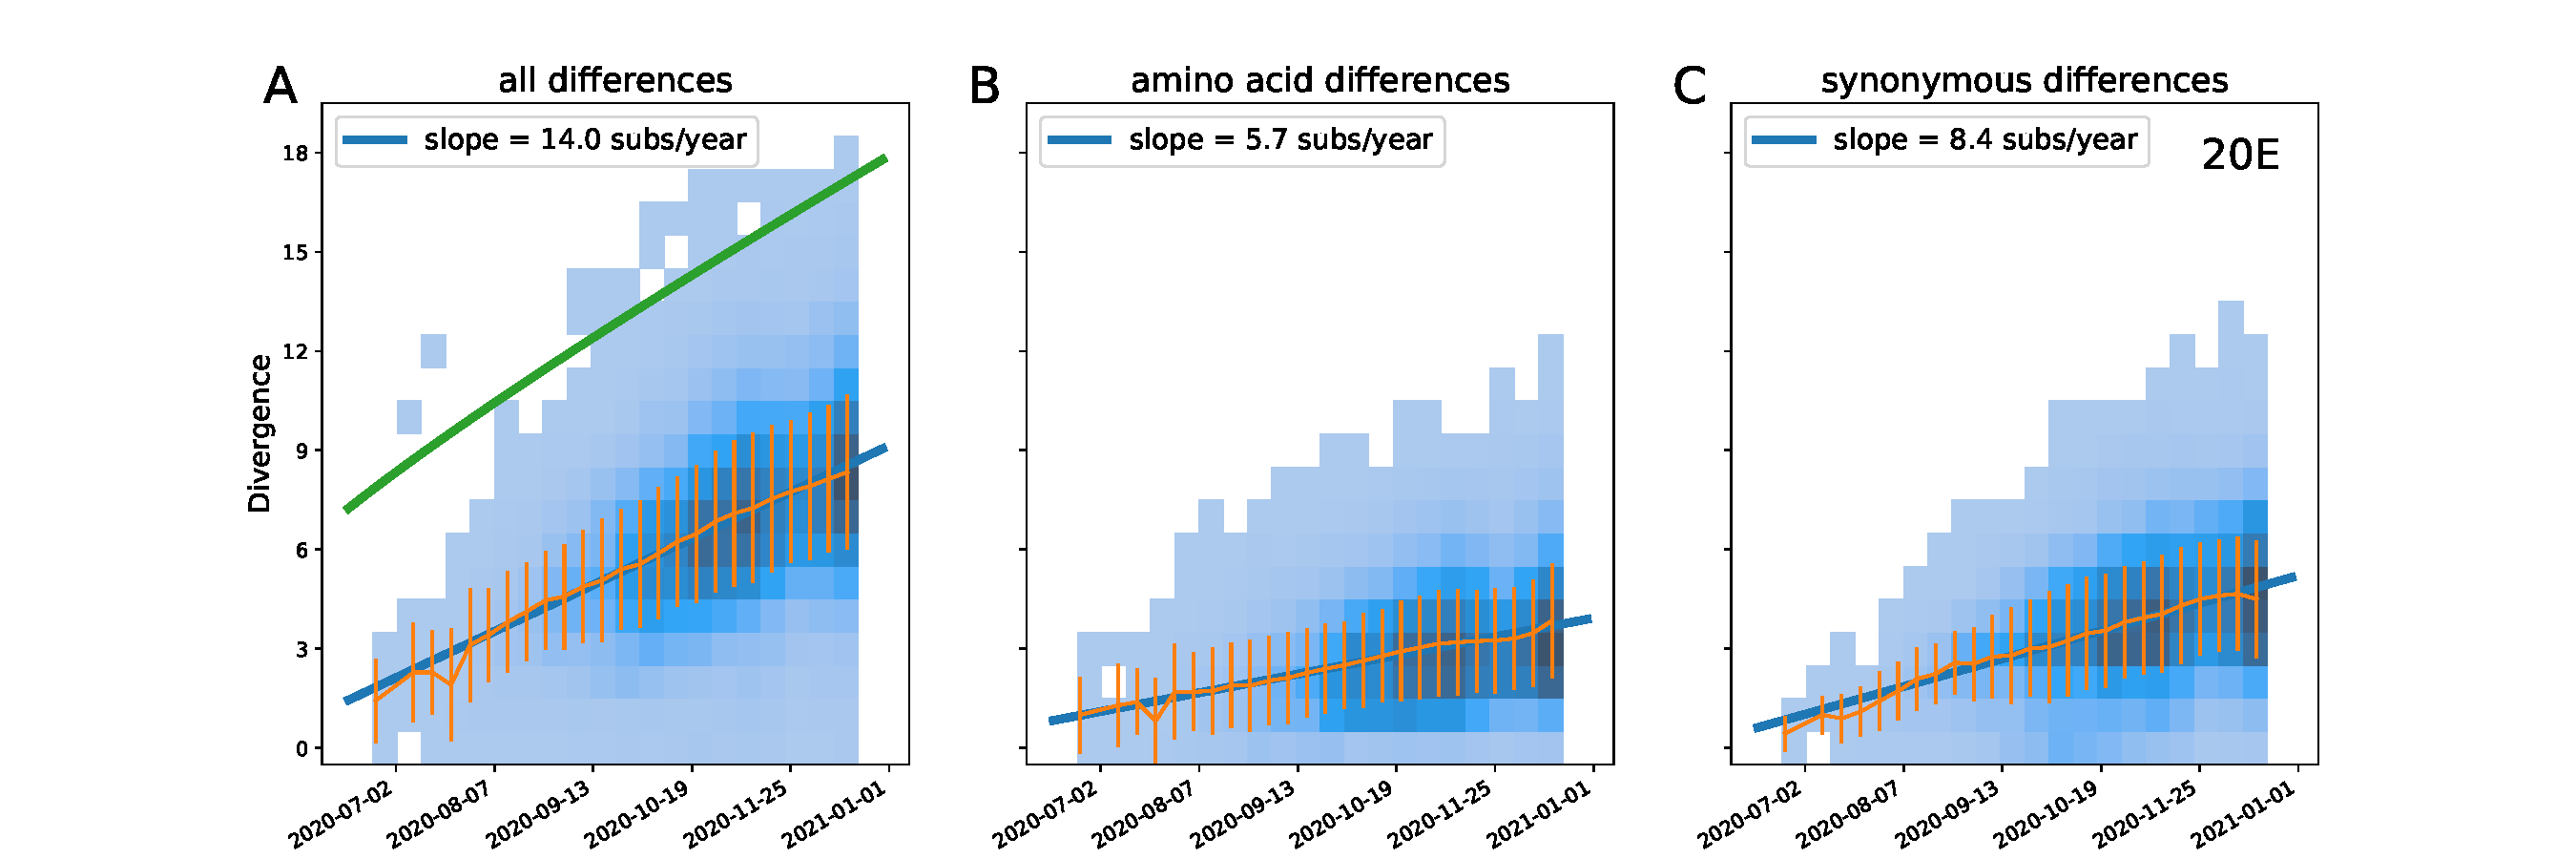
\includegraphics[width=0.8\textwidth]{figures/rtt/20E_rtt.pdf}
    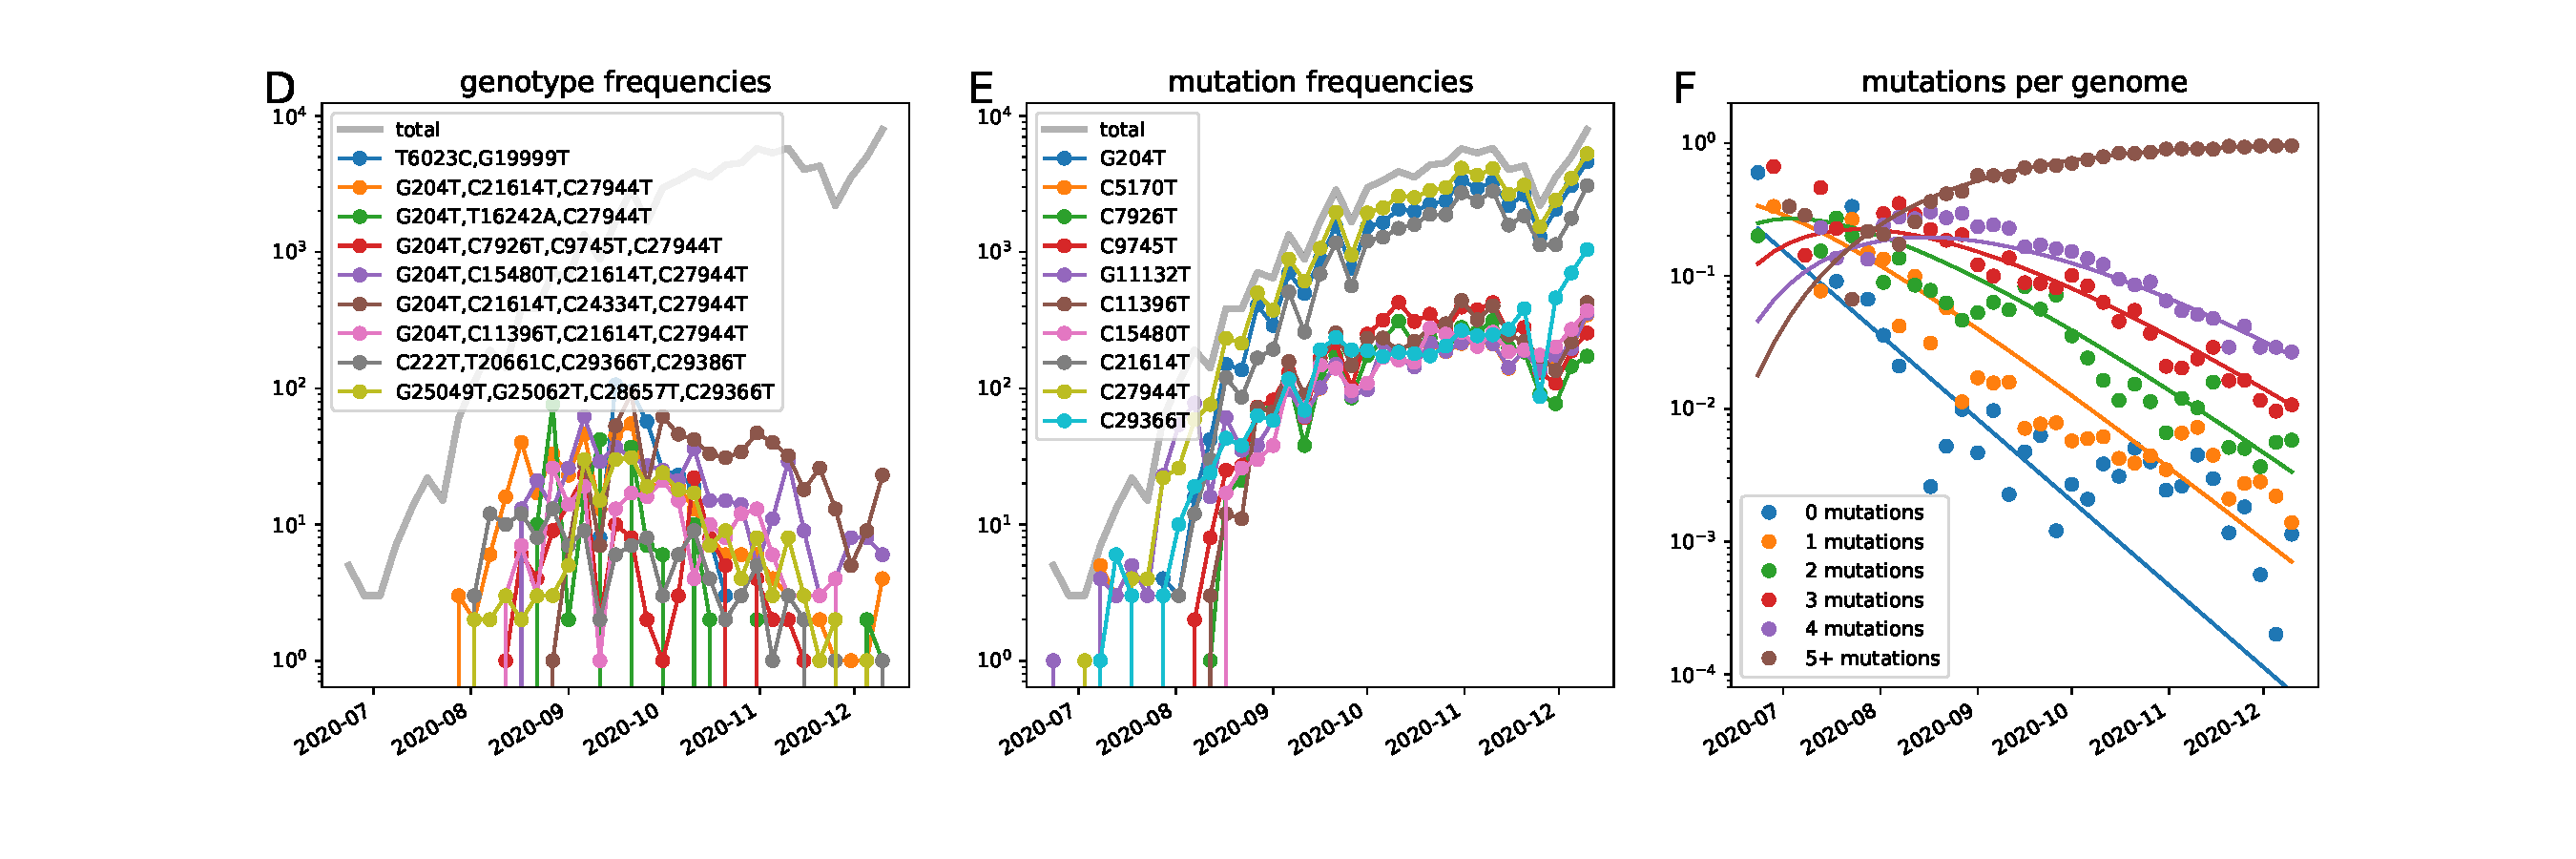
\includegraphics[width=0.8\textwidth]{figures/counts/20E_counts.pdf}
    \caption{{\bf Divergence increases linearly with time in clade 20E.}
    \label{fig:20E_divergence}}
\end{figure*}

\begin{figure*}[h]
    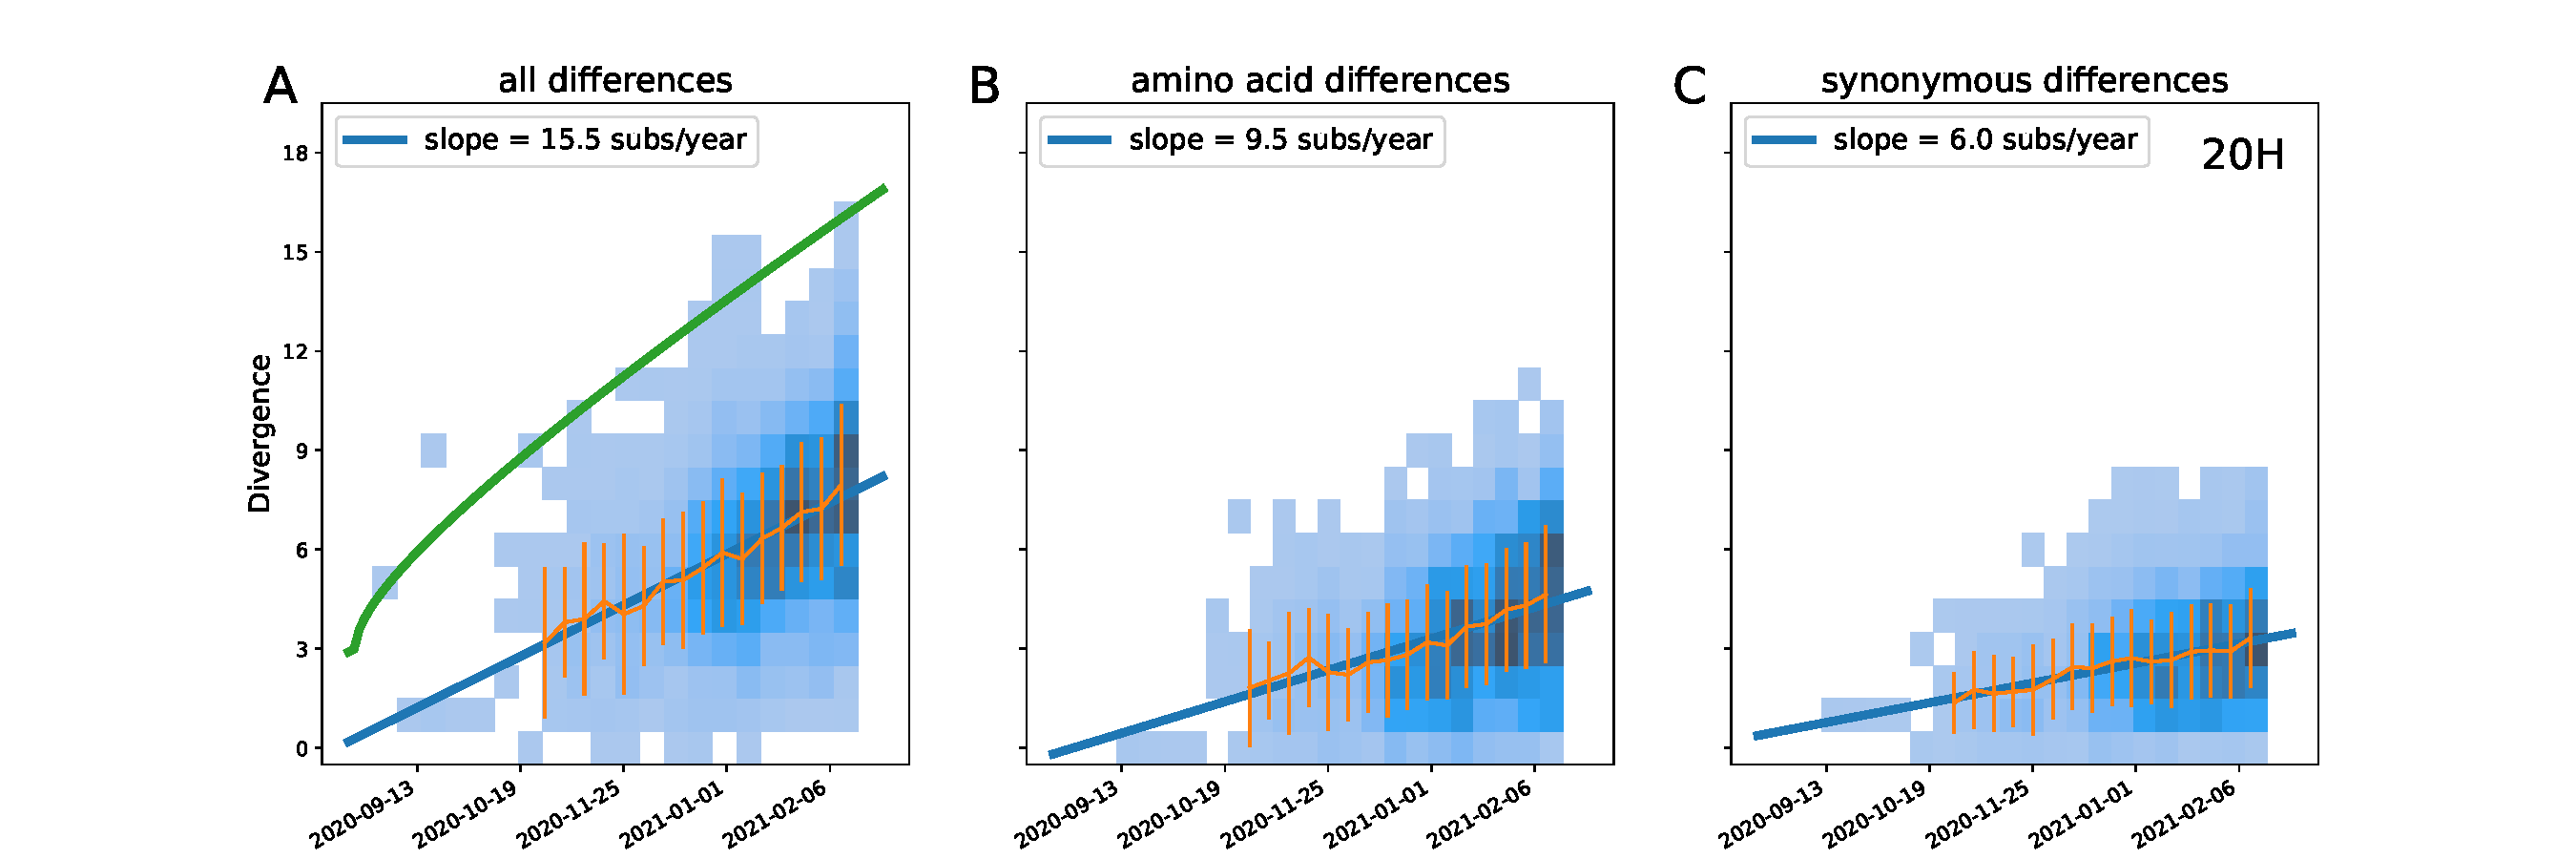
\includegraphics[width=0.8\textwidth]{figures/rtt/20H_rtt.pdf}
    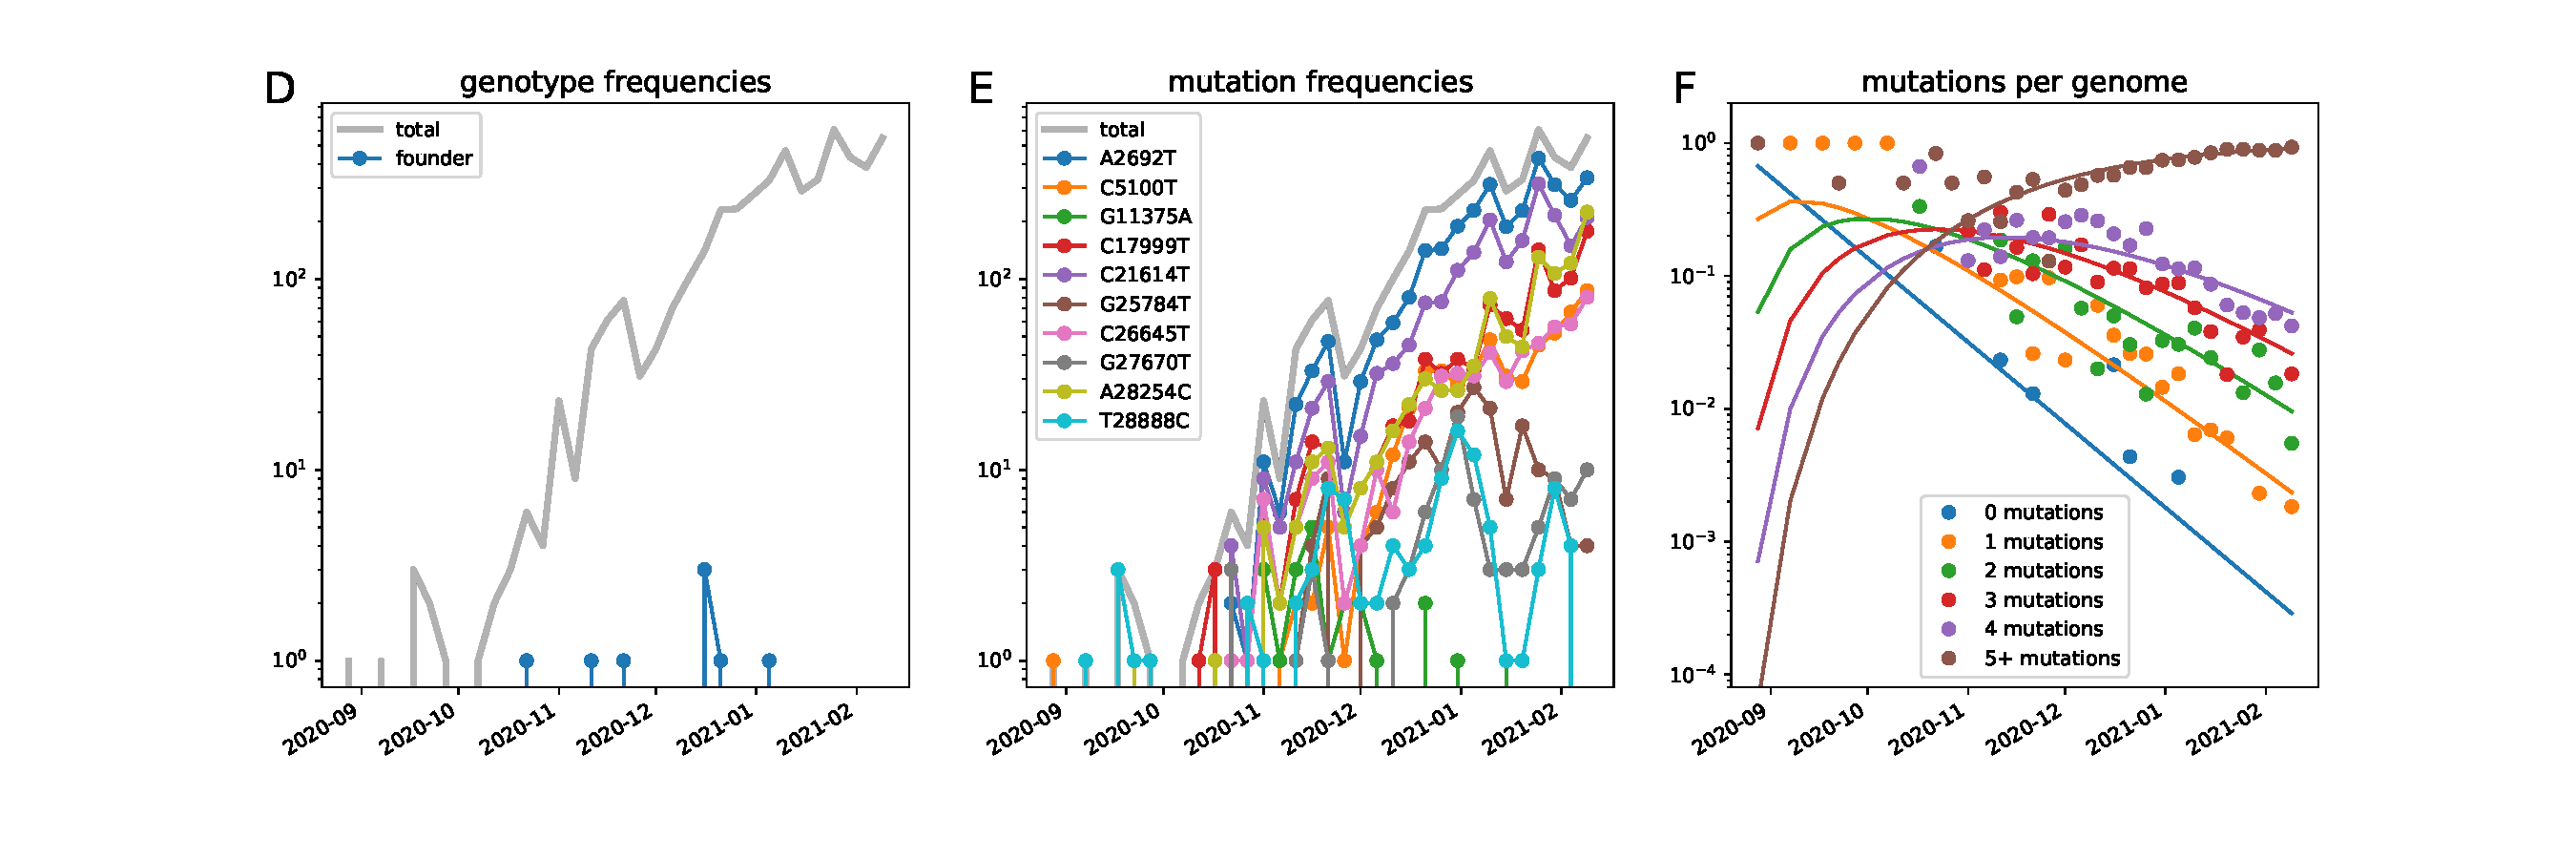
\includegraphics[width=0.8\textwidth]{figures/counts/20H_counts.pdf}
    \caption{{\bf Divergence increases linearly with time in clade 20H (Beta).}
    \label{fig:20H_divergence}}
\end{figure*}

\begin{figure*}[h]
    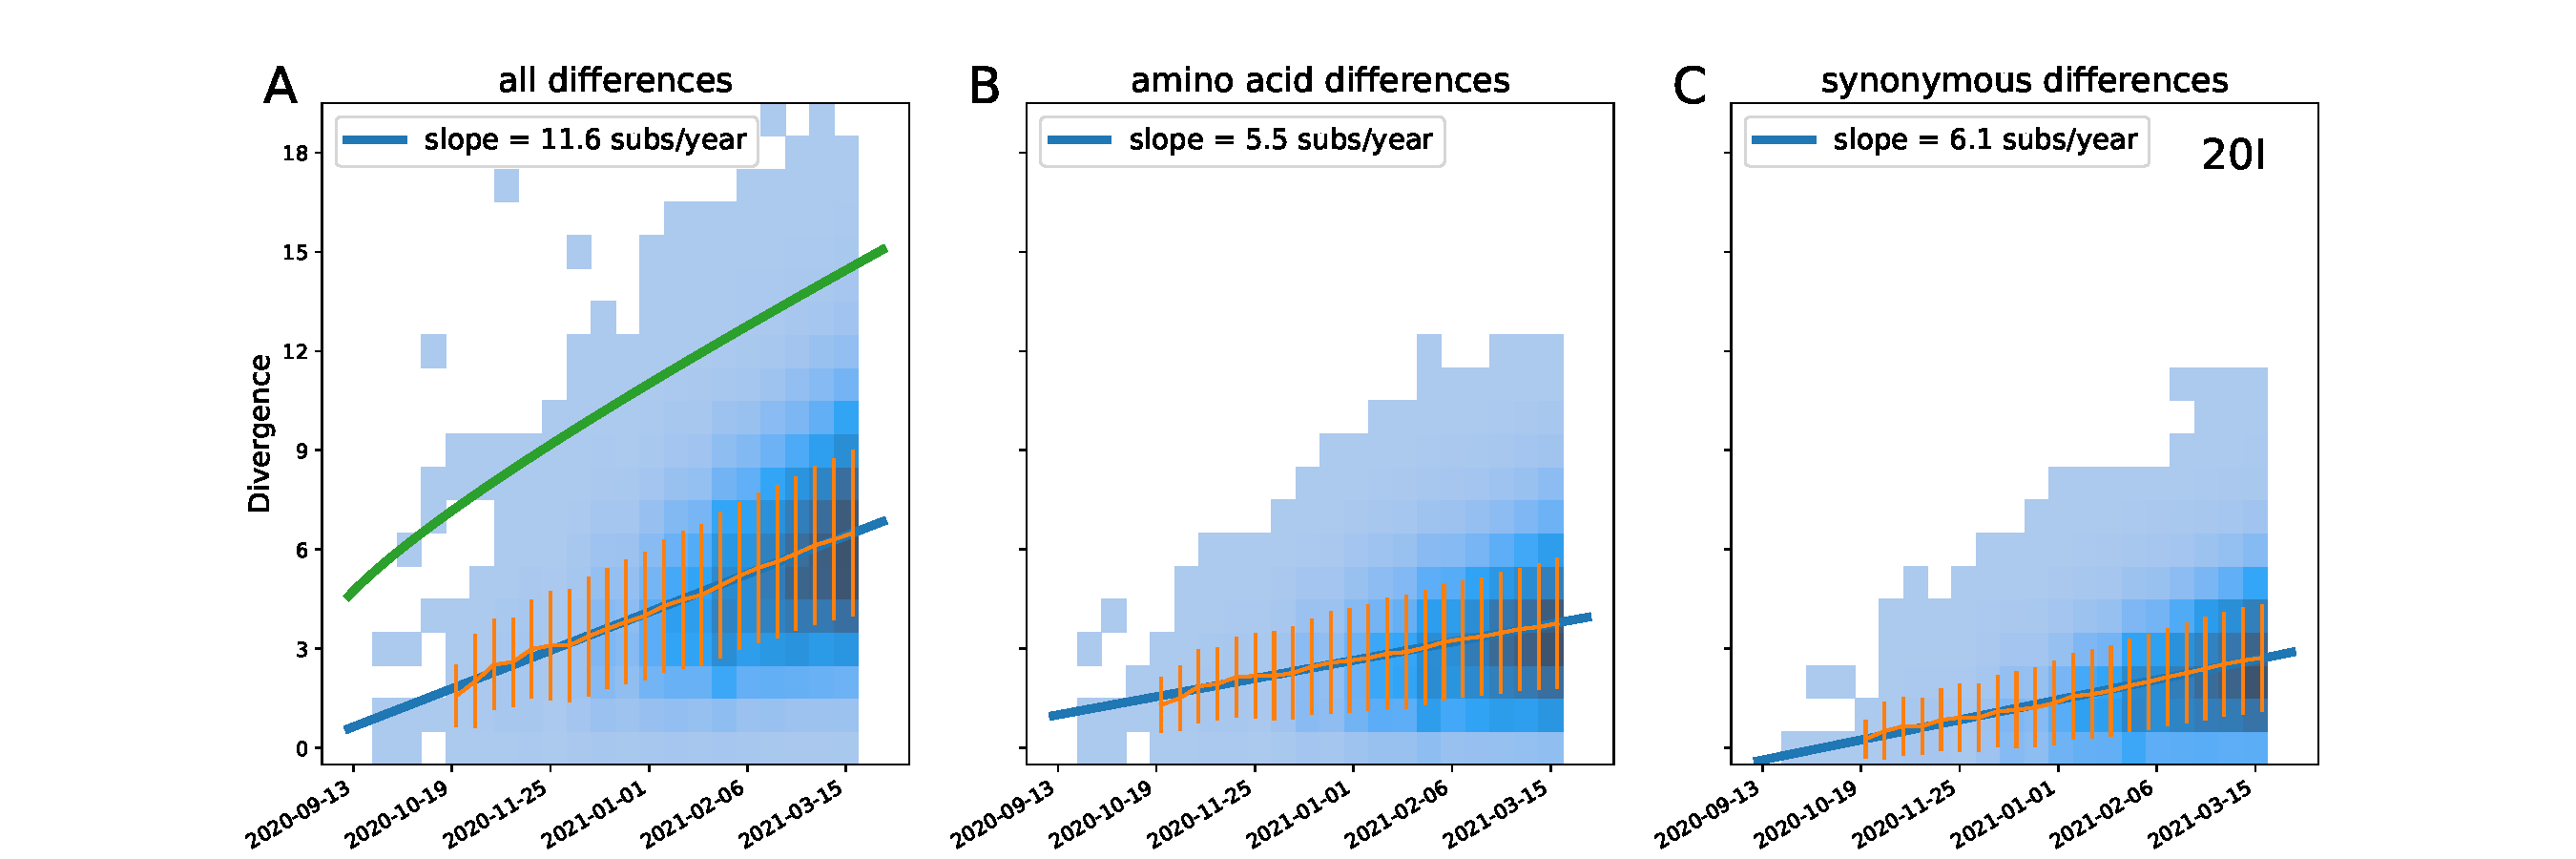
\includegraphics[width=0.8\textwidth]{figures/rtt/20I_rtt.pdf}
    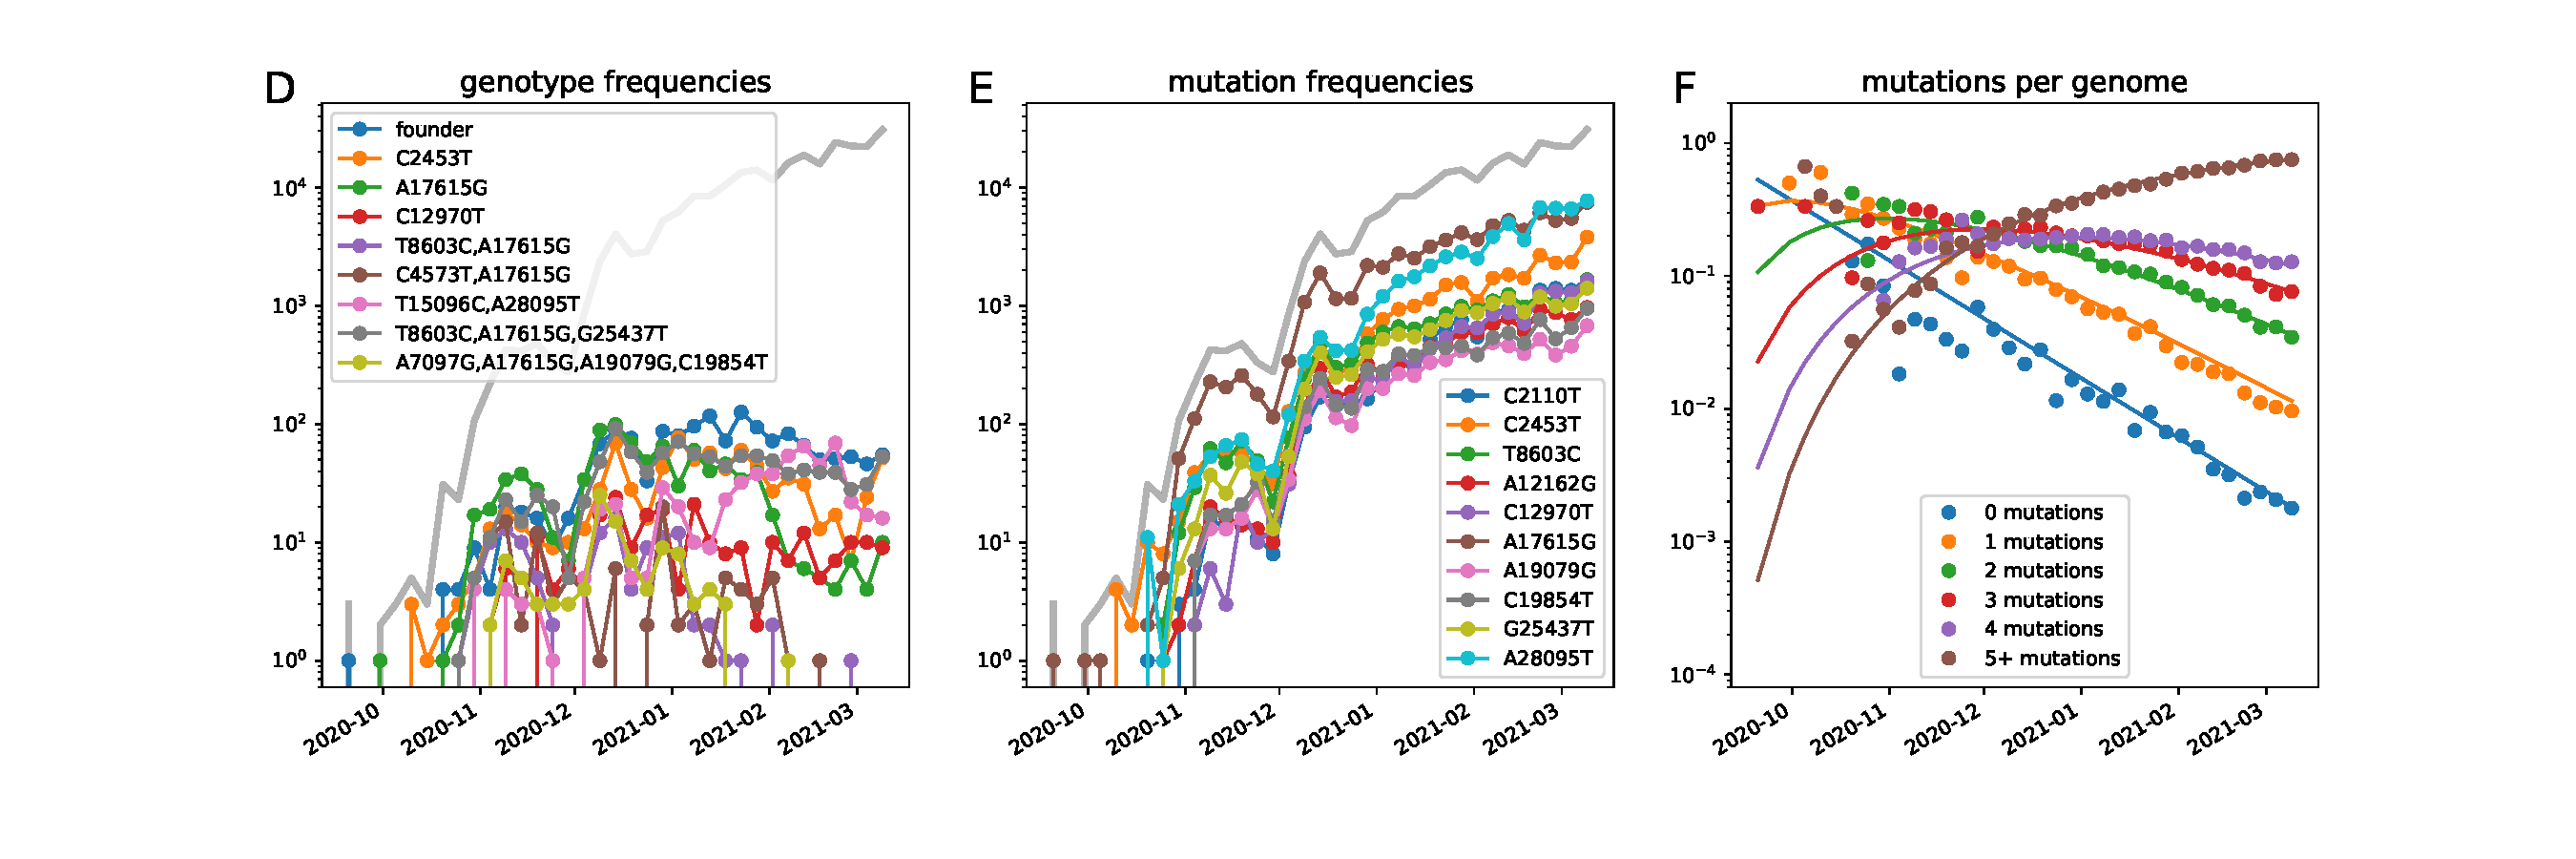
\includegraphics[width=0.8\textwidth]{figures/counts/20I_counts.pdf}
    \caption{{\bf Divergence increases linearly with time in clade 20I (Alpha).}
    \label{fig:20I_divergence}}
\end{figure*}

\begin{figure*}[h]
    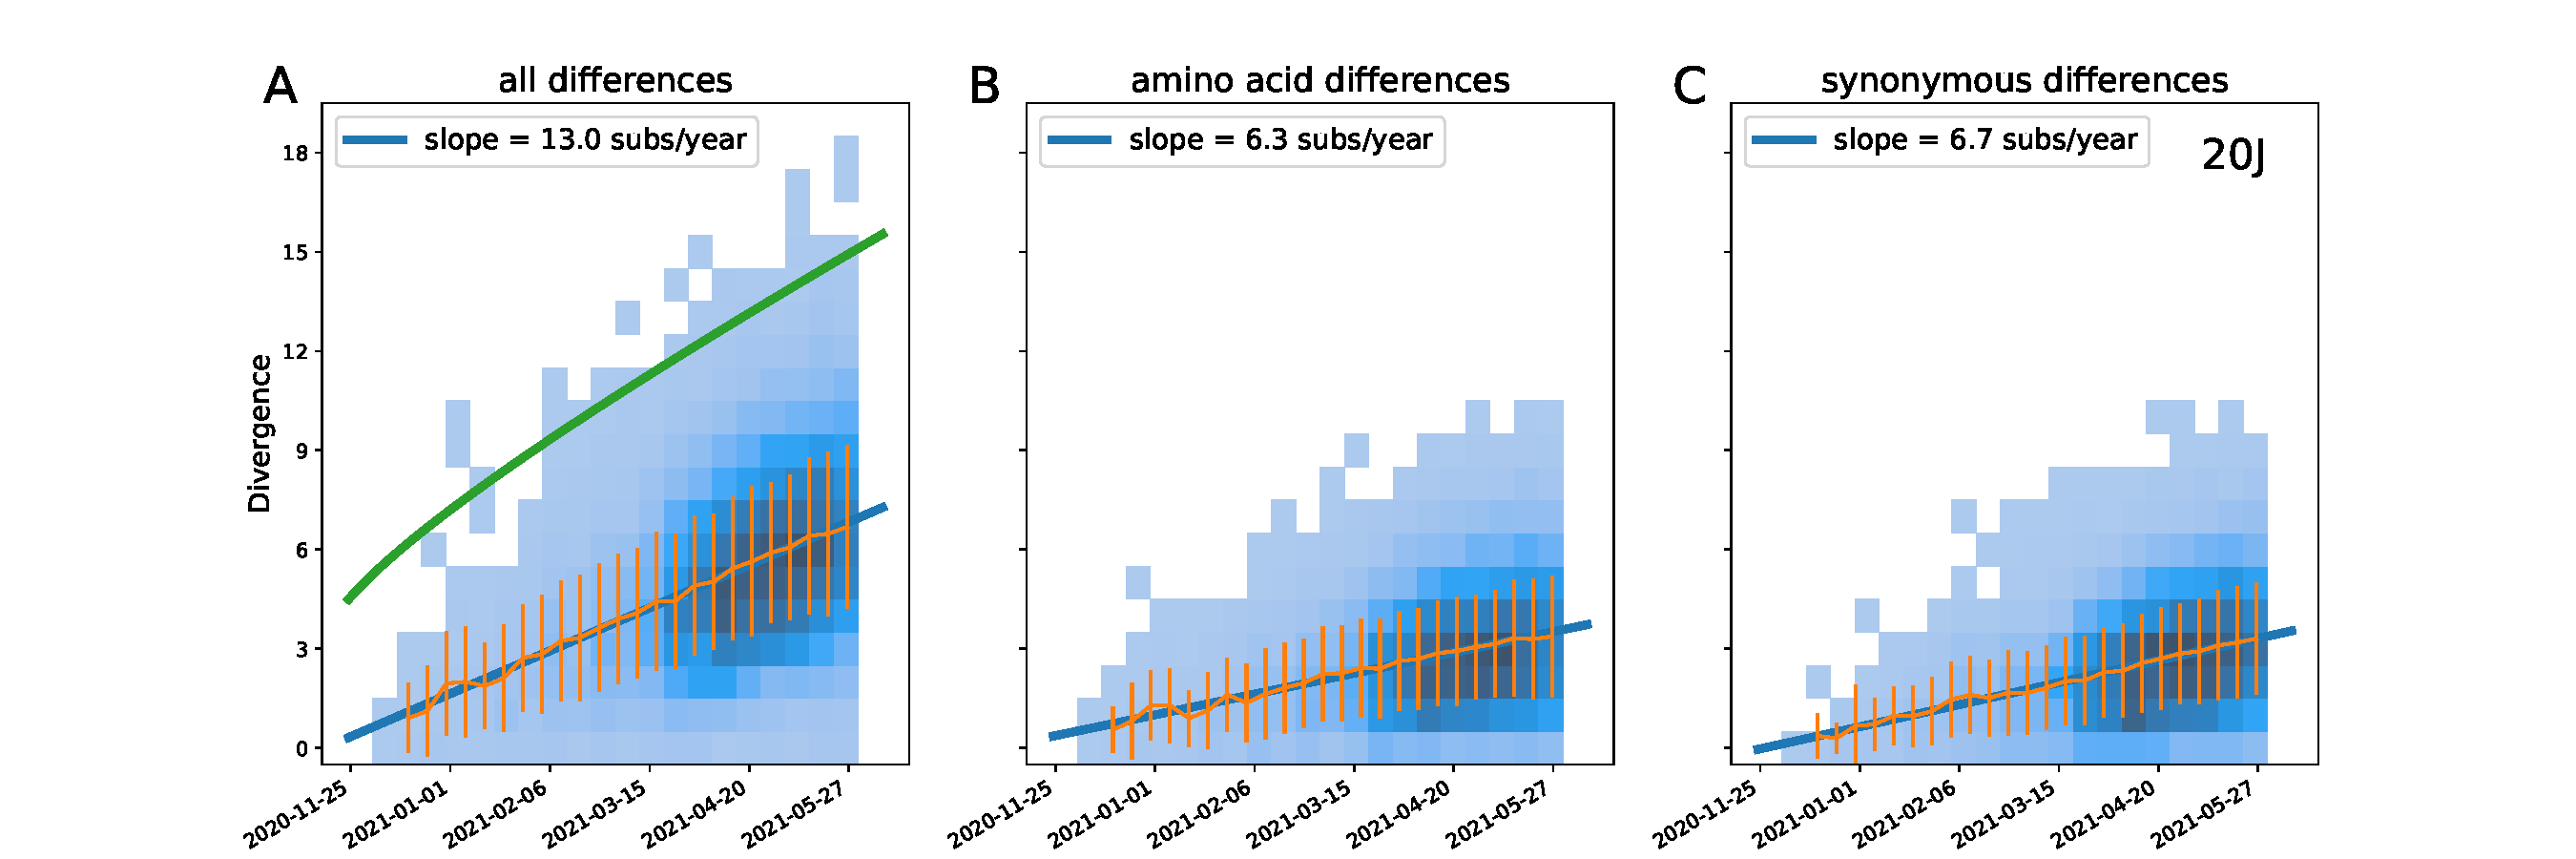
\includegraphics[width=0.8\textwidth]{figures/rtt/20J_rtt.pdf}
    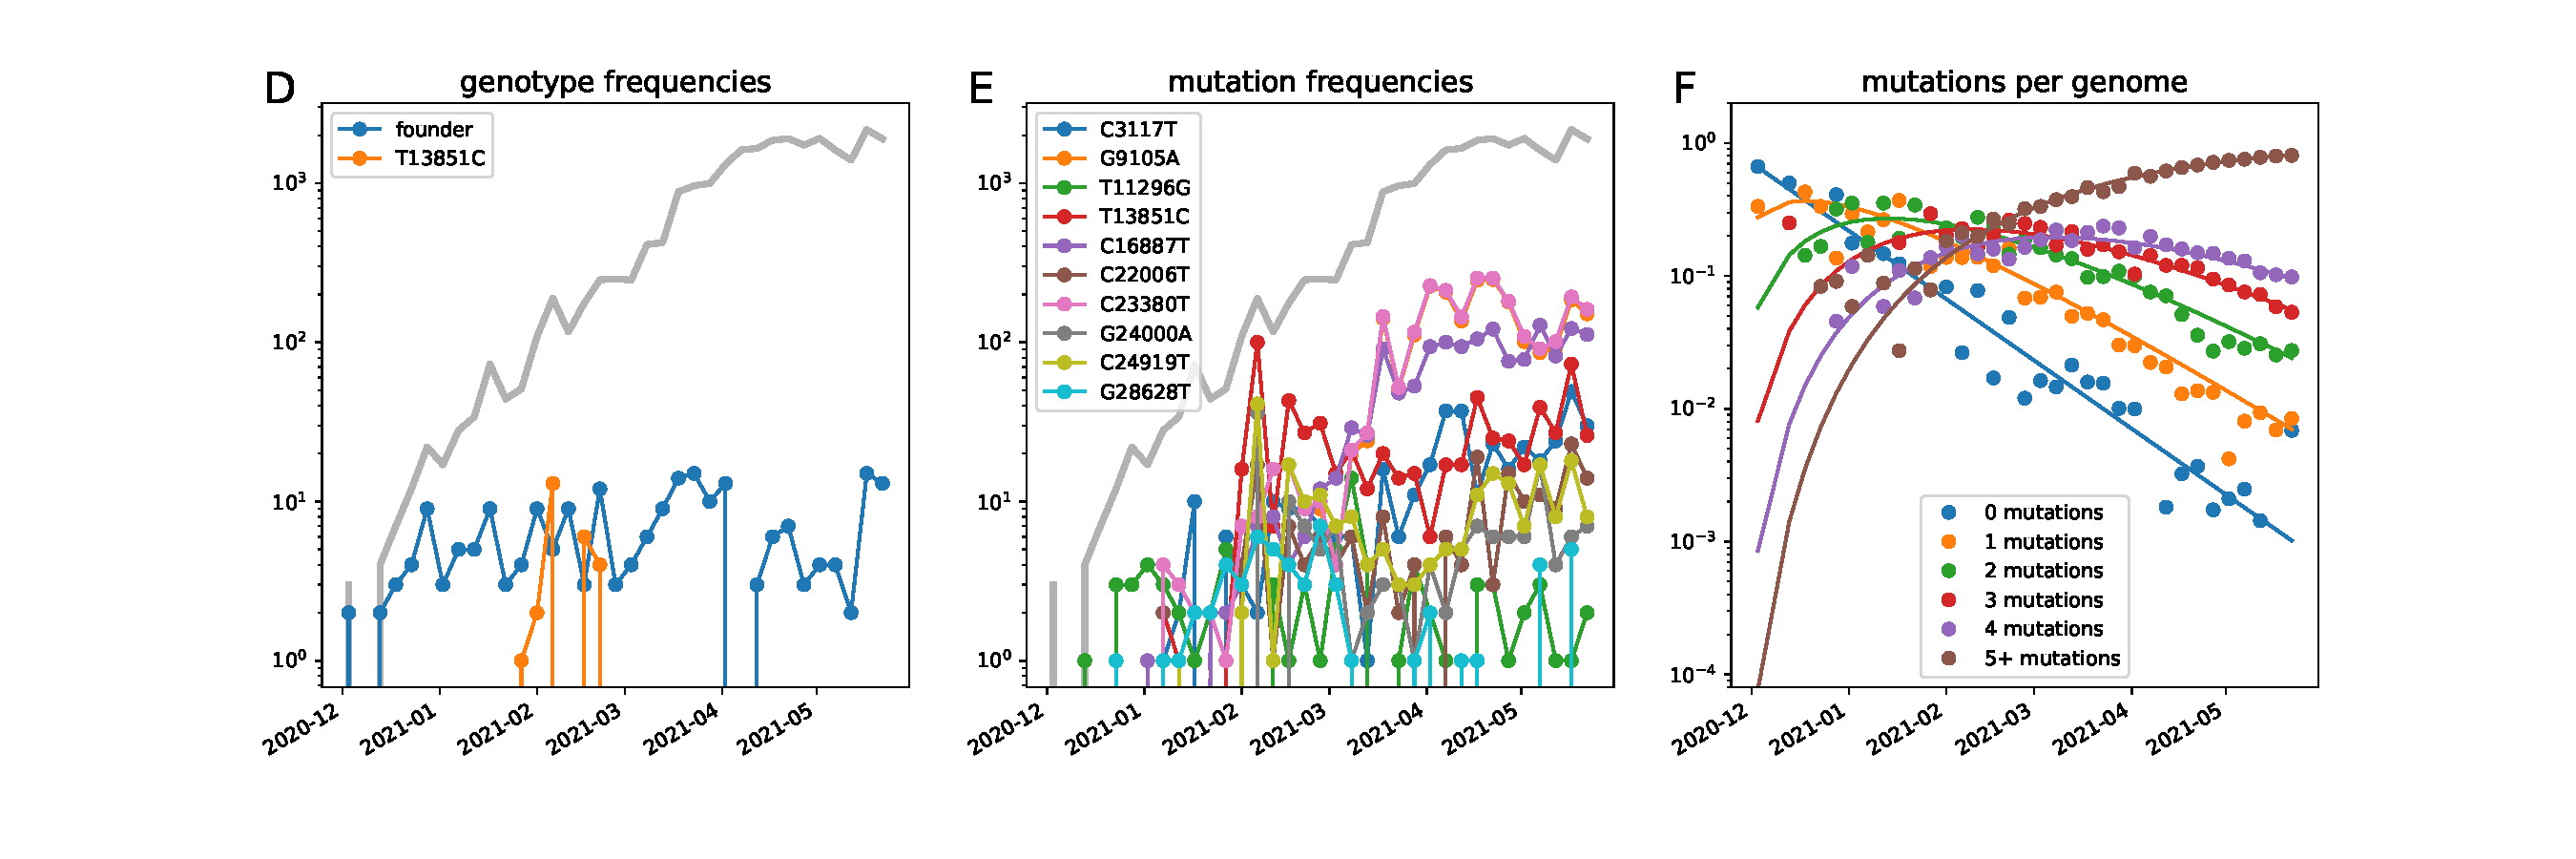
\includegraphics[width=0.8\textwidth]{figures/counts/20J_counts.pdf}
    \caption{{\bf Divergence increases linearly with time in clade 20J (Gamma).}
    \label{fig:20J_divergence}}
\end{figure*}


\begin{figure*}[h]
    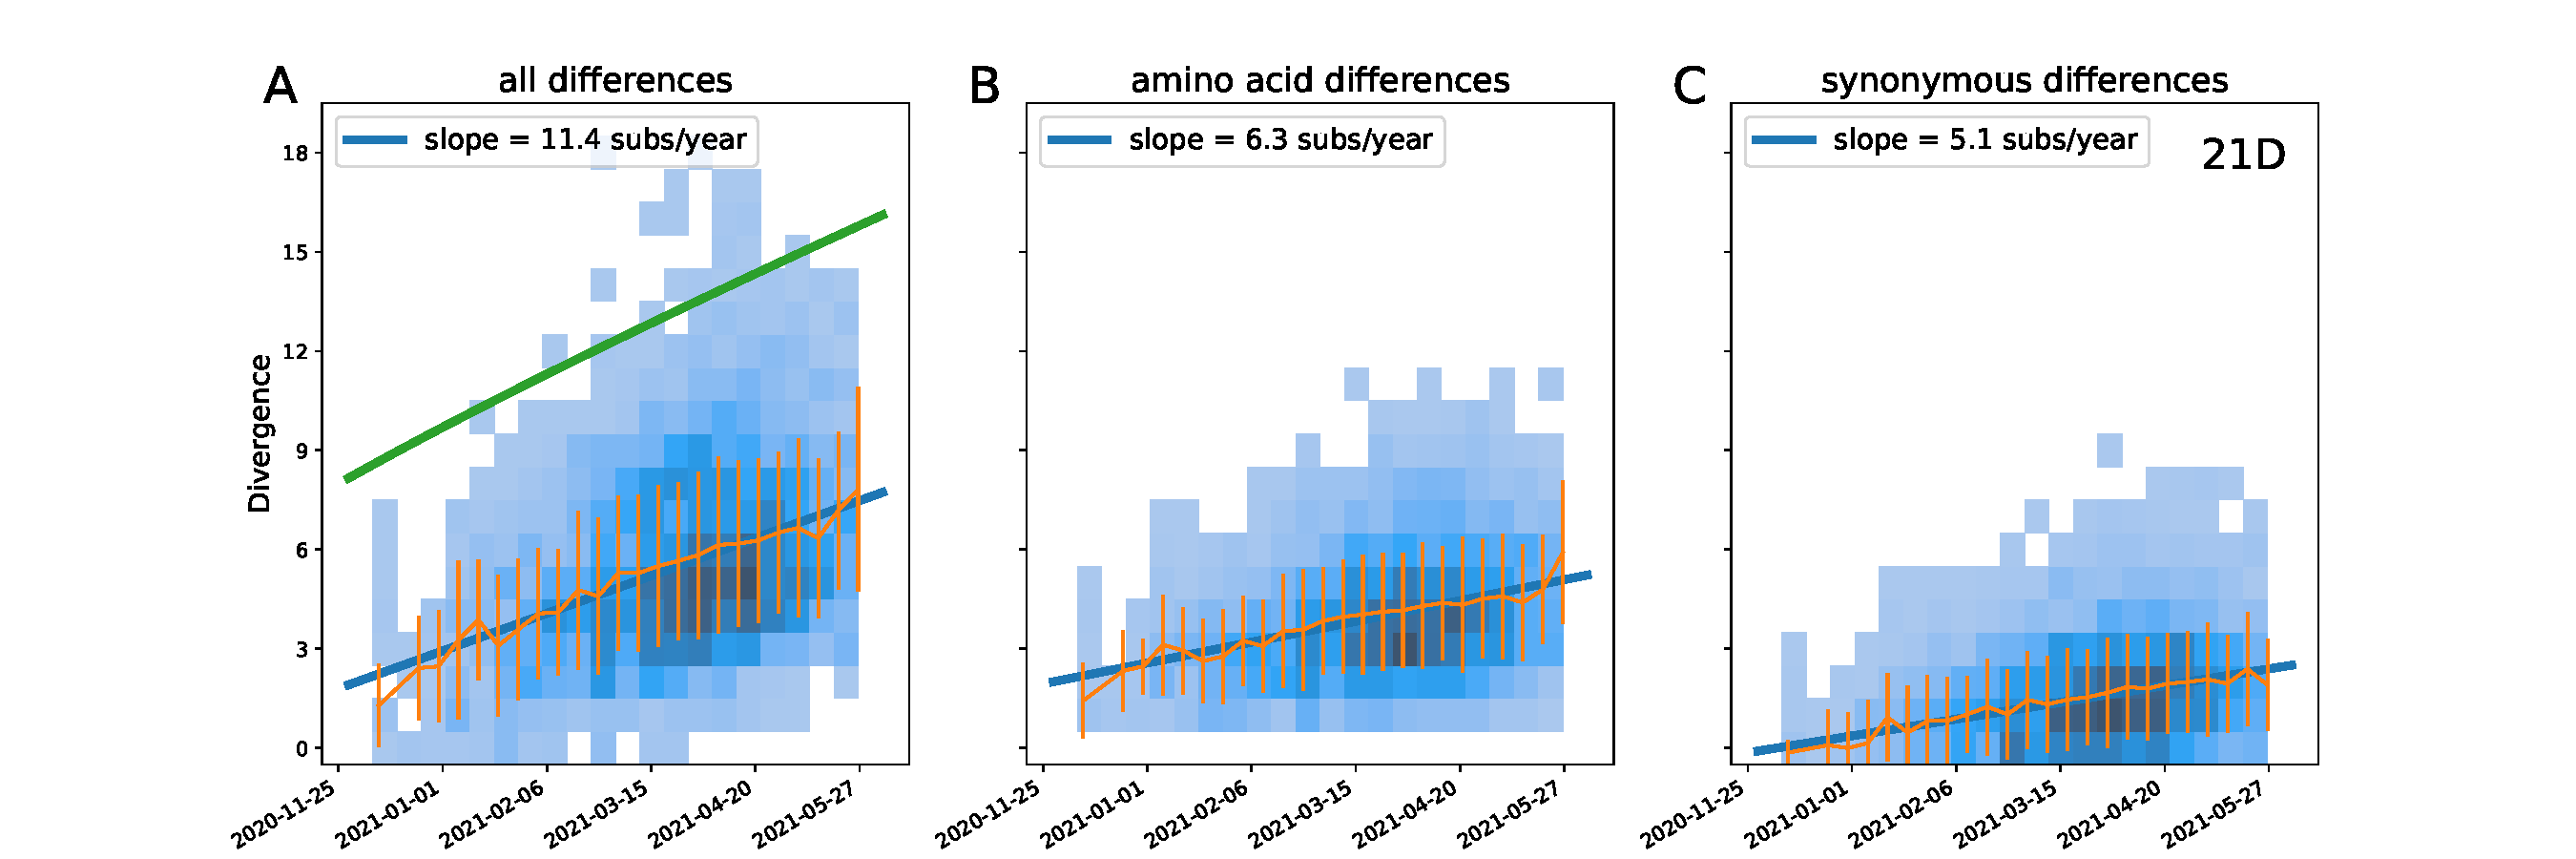
\includegraphics[width=0.8\textwidth]{figures/rtt/21D_rtt.pdf}
    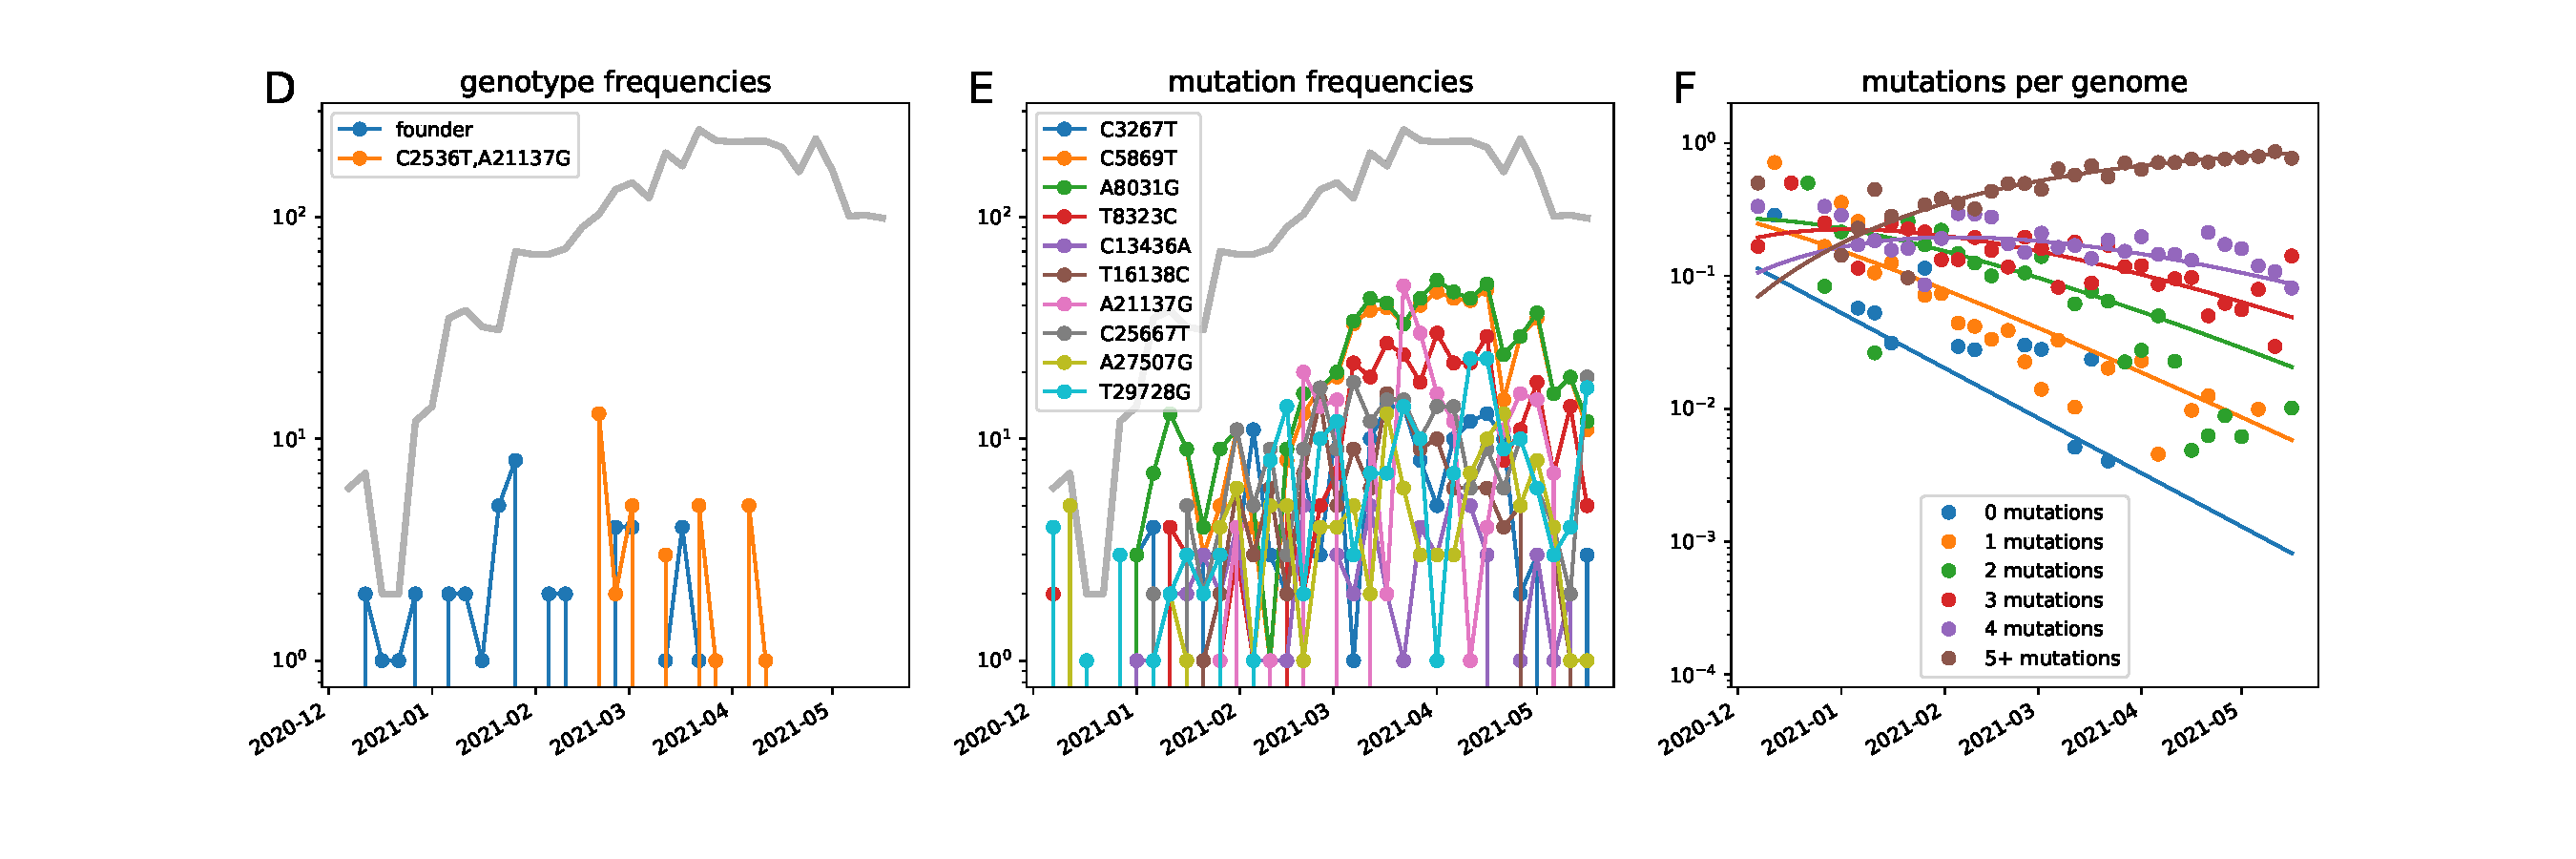
\includegraphics[width=0.8\textwidth]{figures/counts/21D_counts.pdf}
    \caption{{\bf Divergence increases linearly with time in clade 21D (Eta).}
    \label{fig:21D_divergence}}
\end{figure*}

\begin{figure*}[h]
    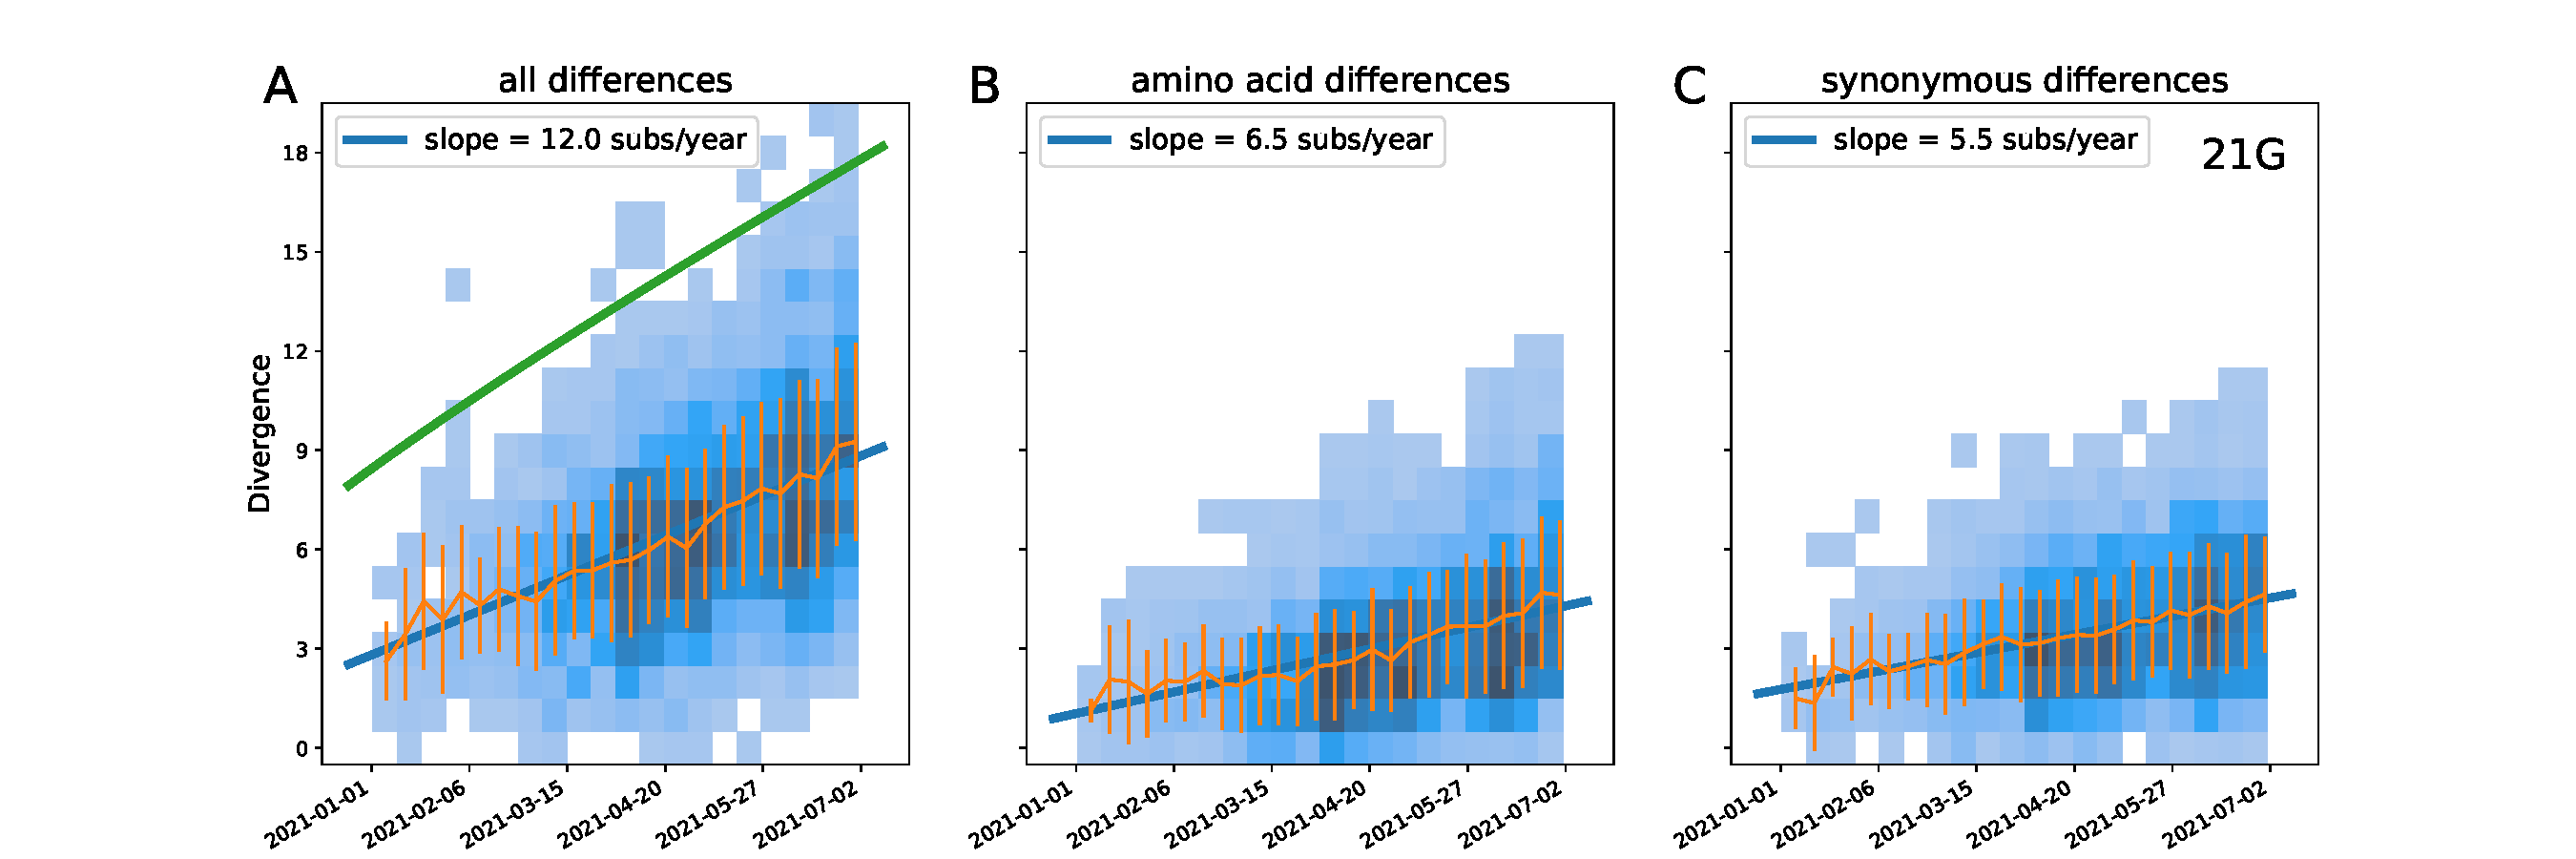
\includegraphics[width=0.8\textwidth]{figures/rtt/21G_rtt.pdf}
    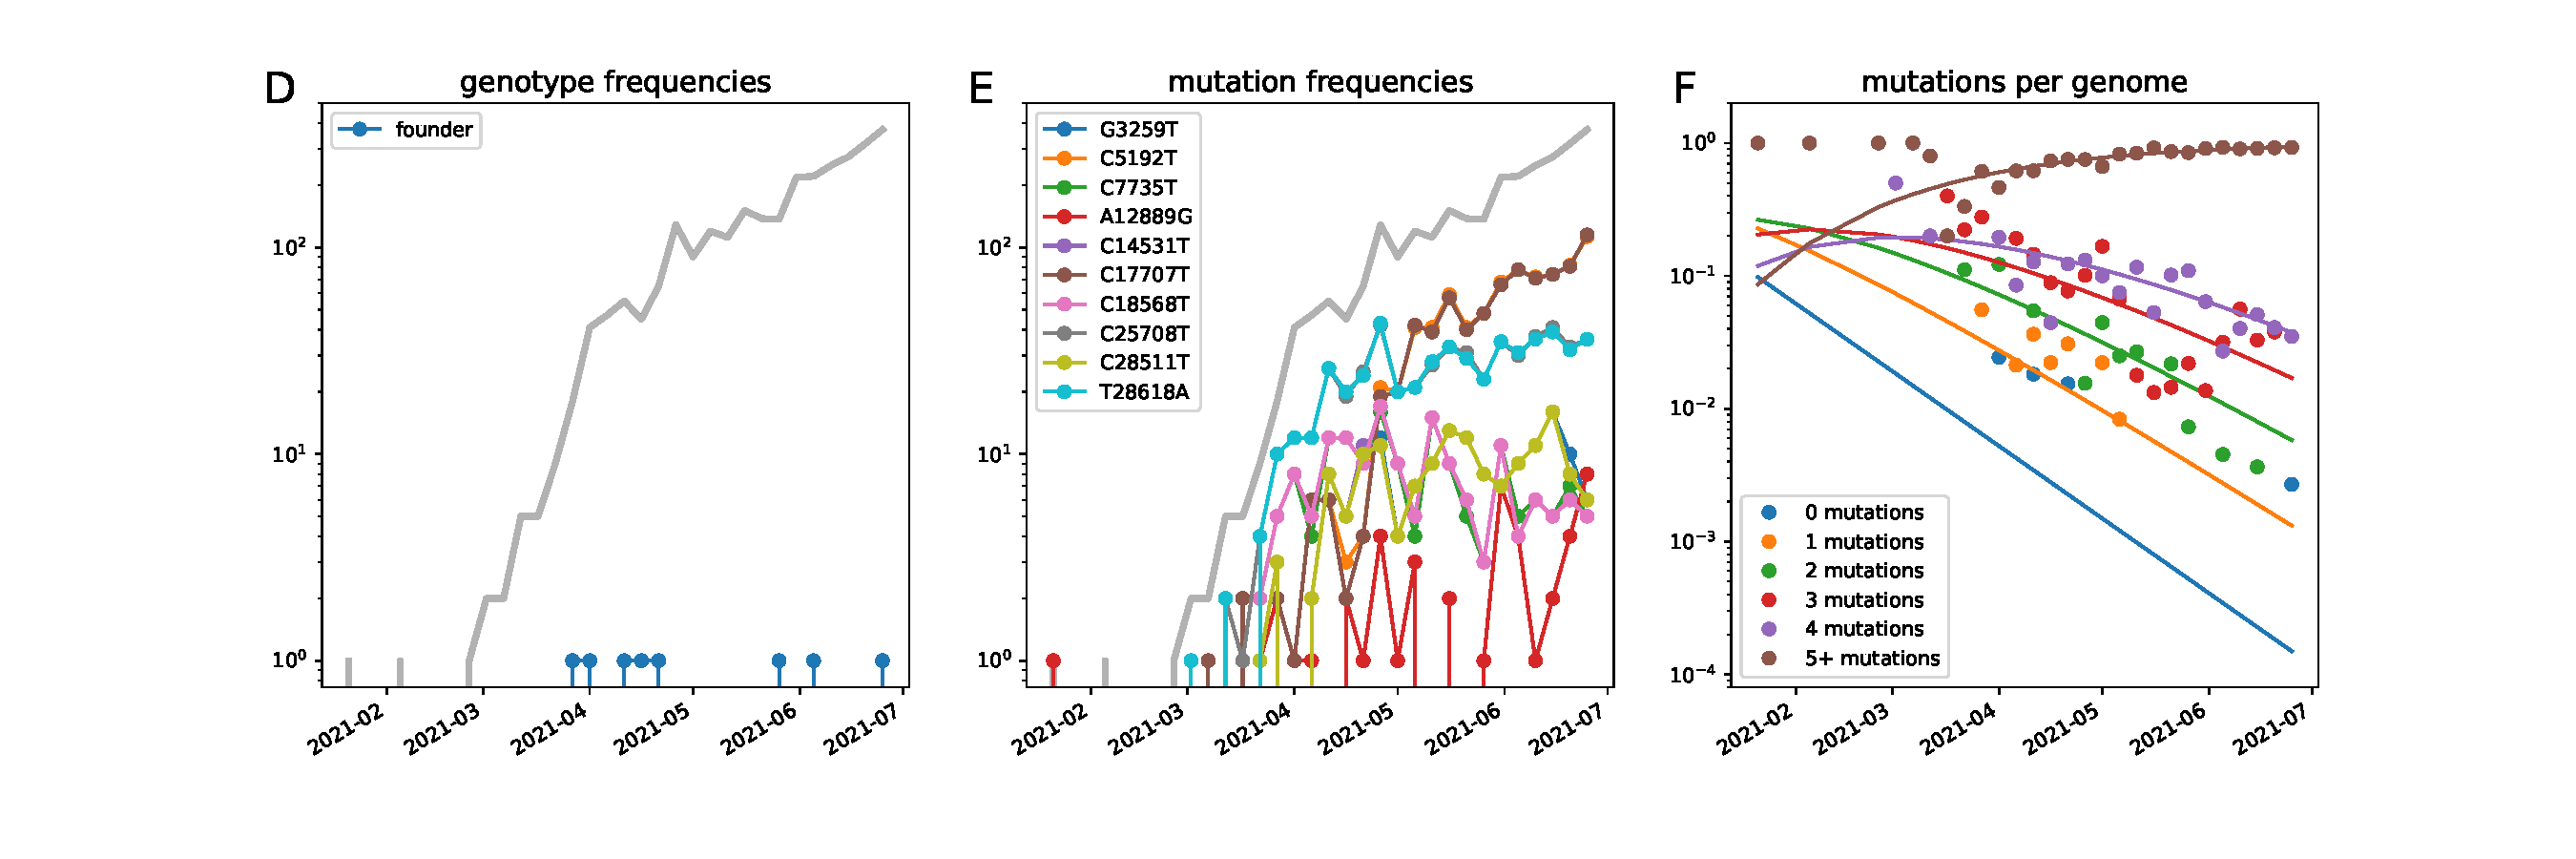
\includegraphics[width=0.8\textwidth]{figures/counts/21H_counts.pdf}
    \caption{{\bf Divergence increases linearly with time in clade 21G (Lambda).}
    \label{fig:21G_divergence}}
\end{figure*}

\begin{figure*}[h]
    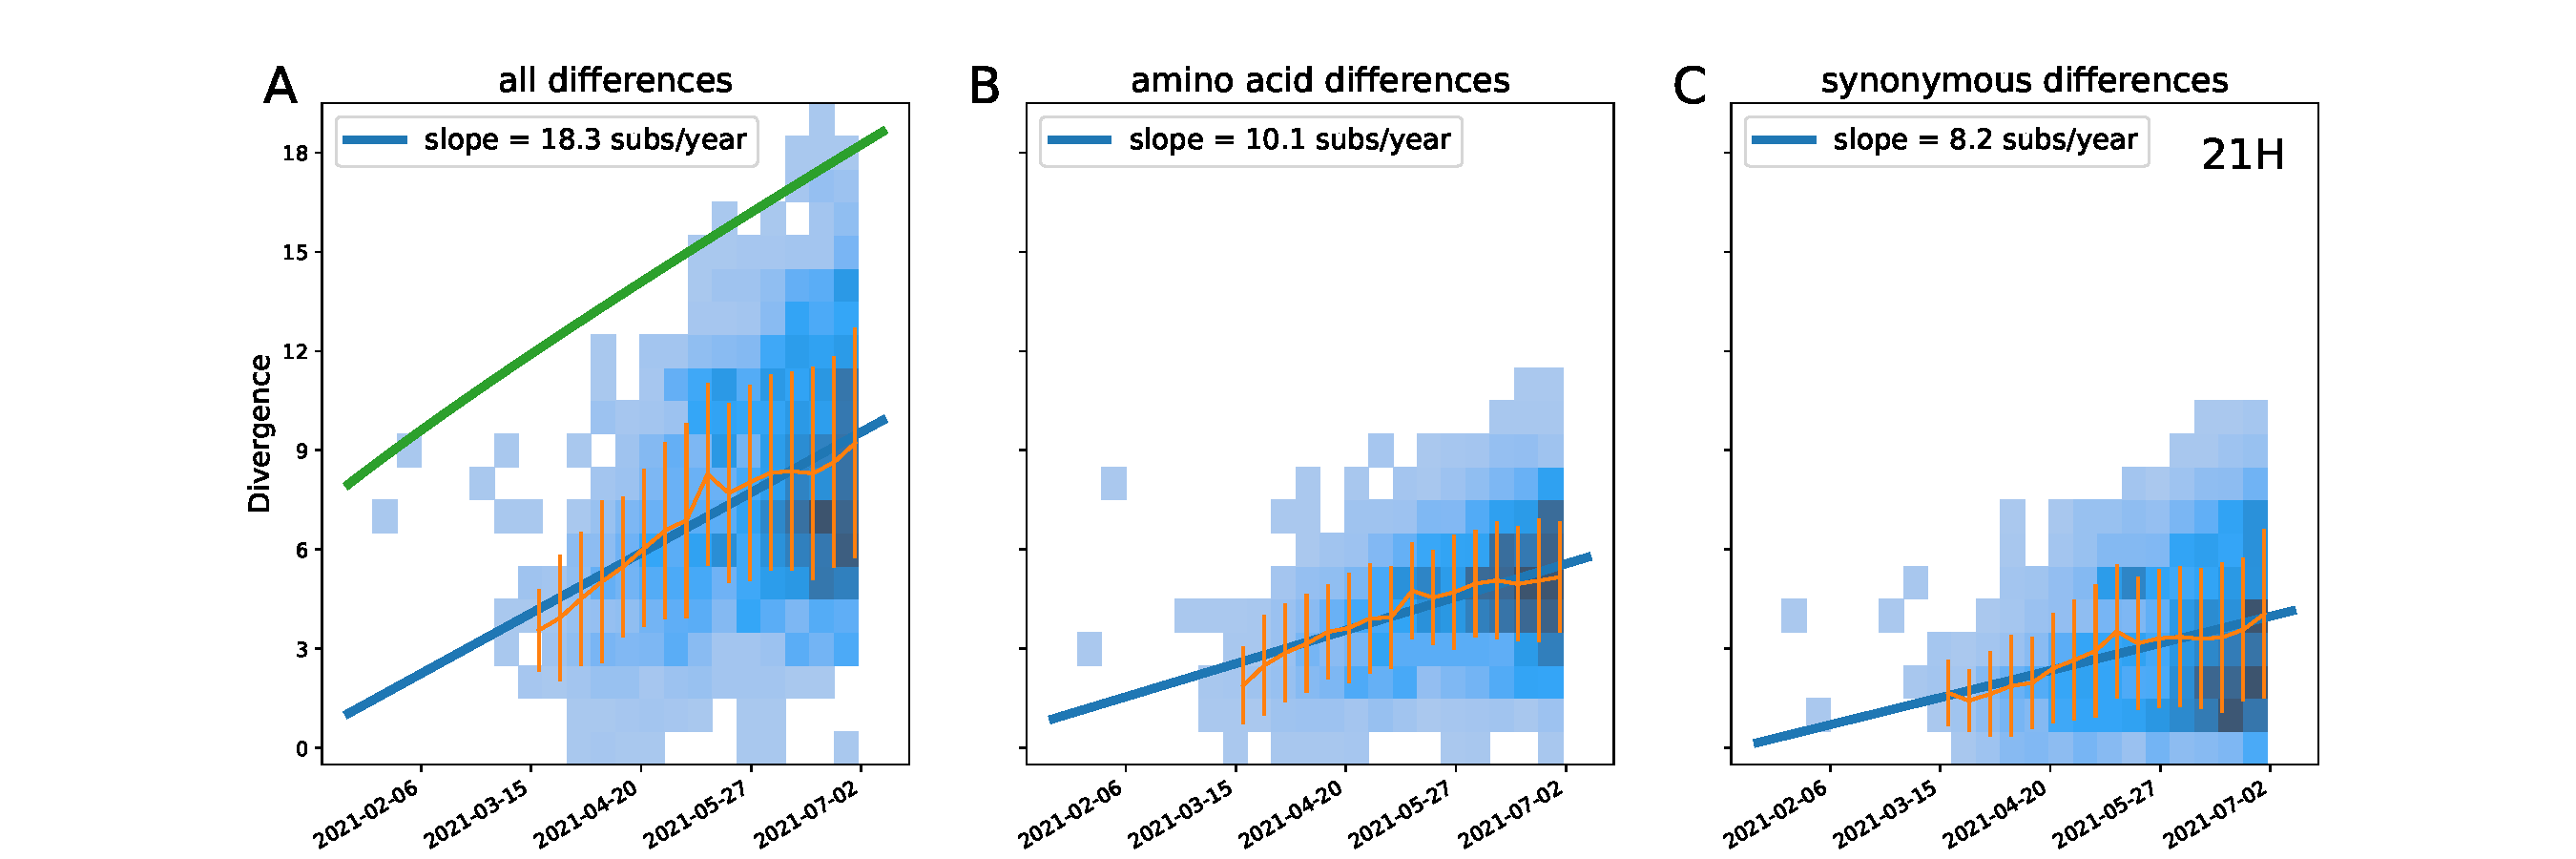
\includegraphics[width=0.8\textwidth]{figures/rtt/21H_rtt.pdf}
    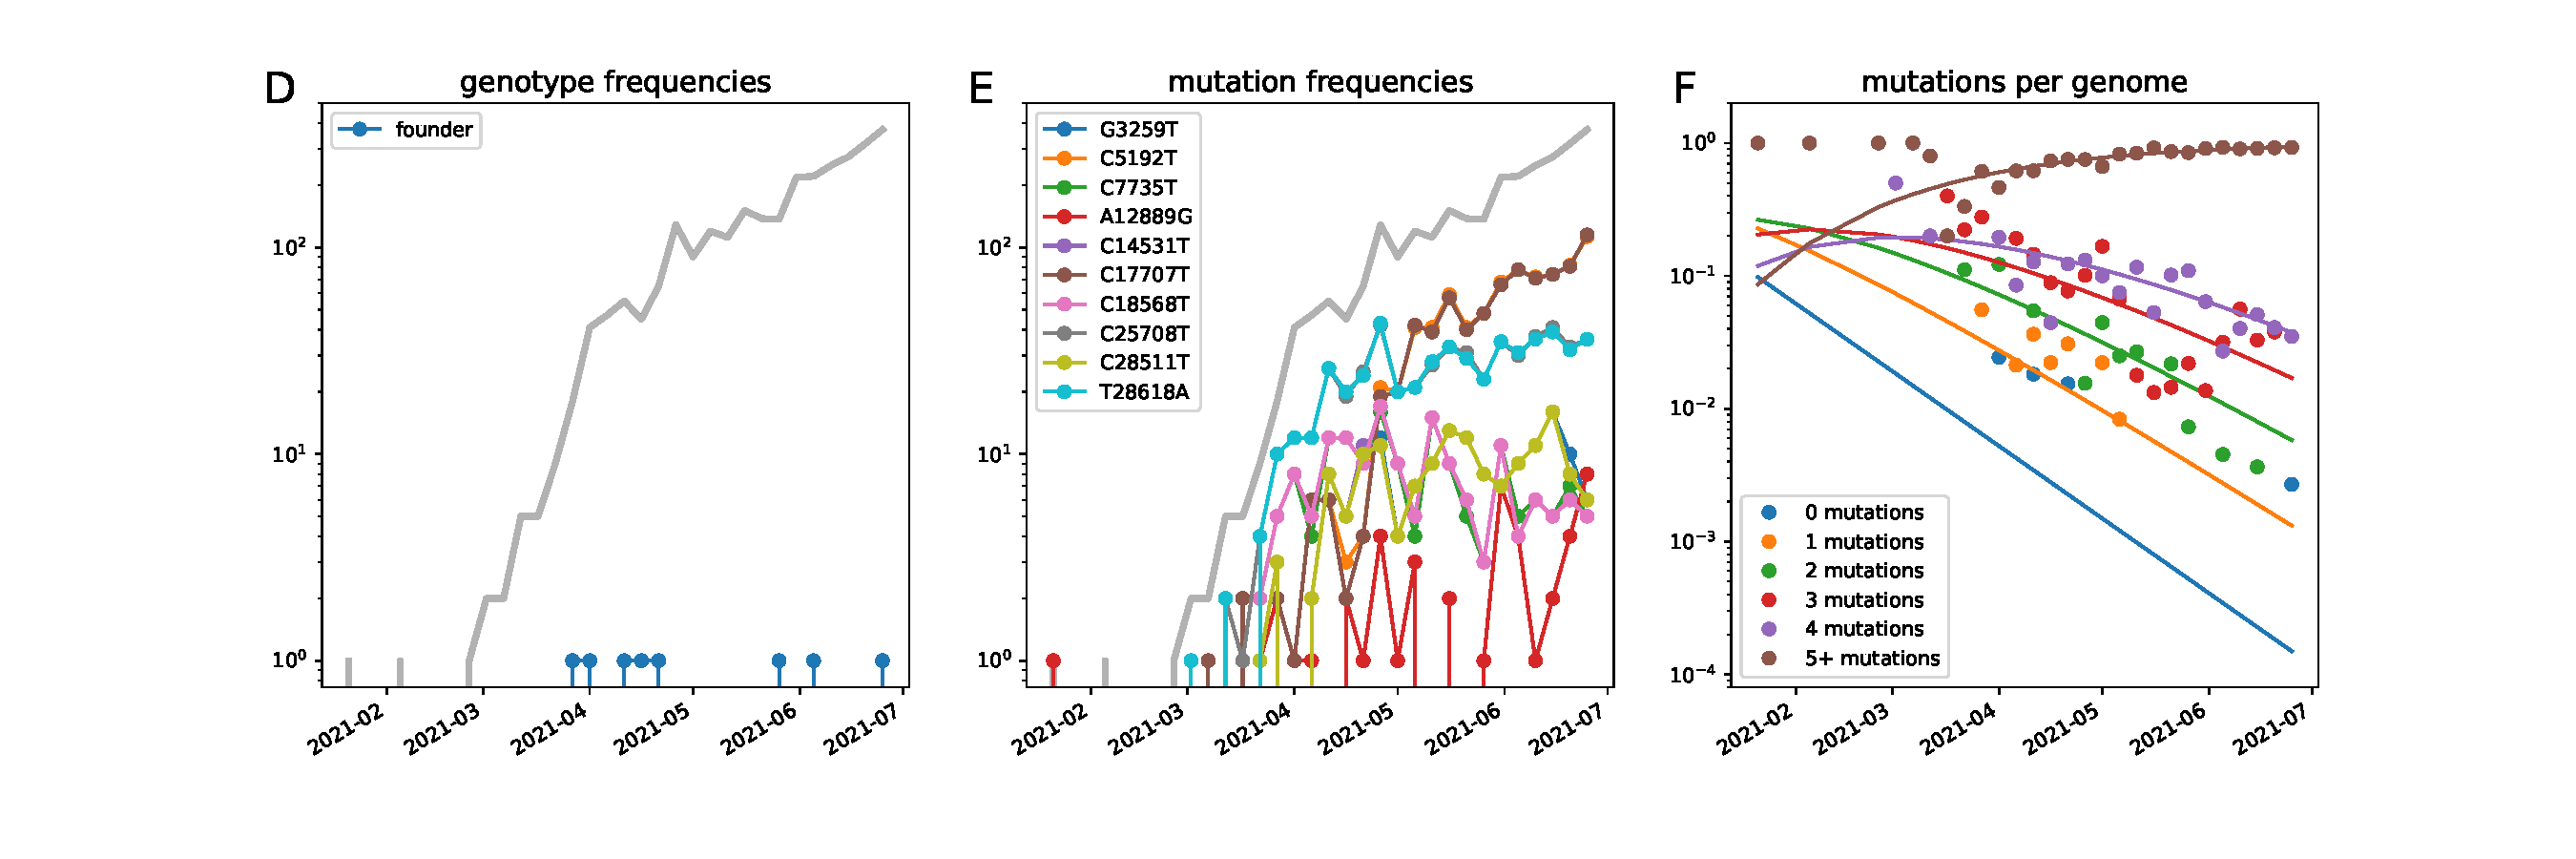
\includegraphics[width=0.8\textwidth]{figures/counts/21H_counts.pdf}
    \caption{{\bf Divergence increases linearly with time in clade 21H (Mu).}
    \label{fig:21H_divergence}}
\end{figure*}

\begin{figure*}[h]
    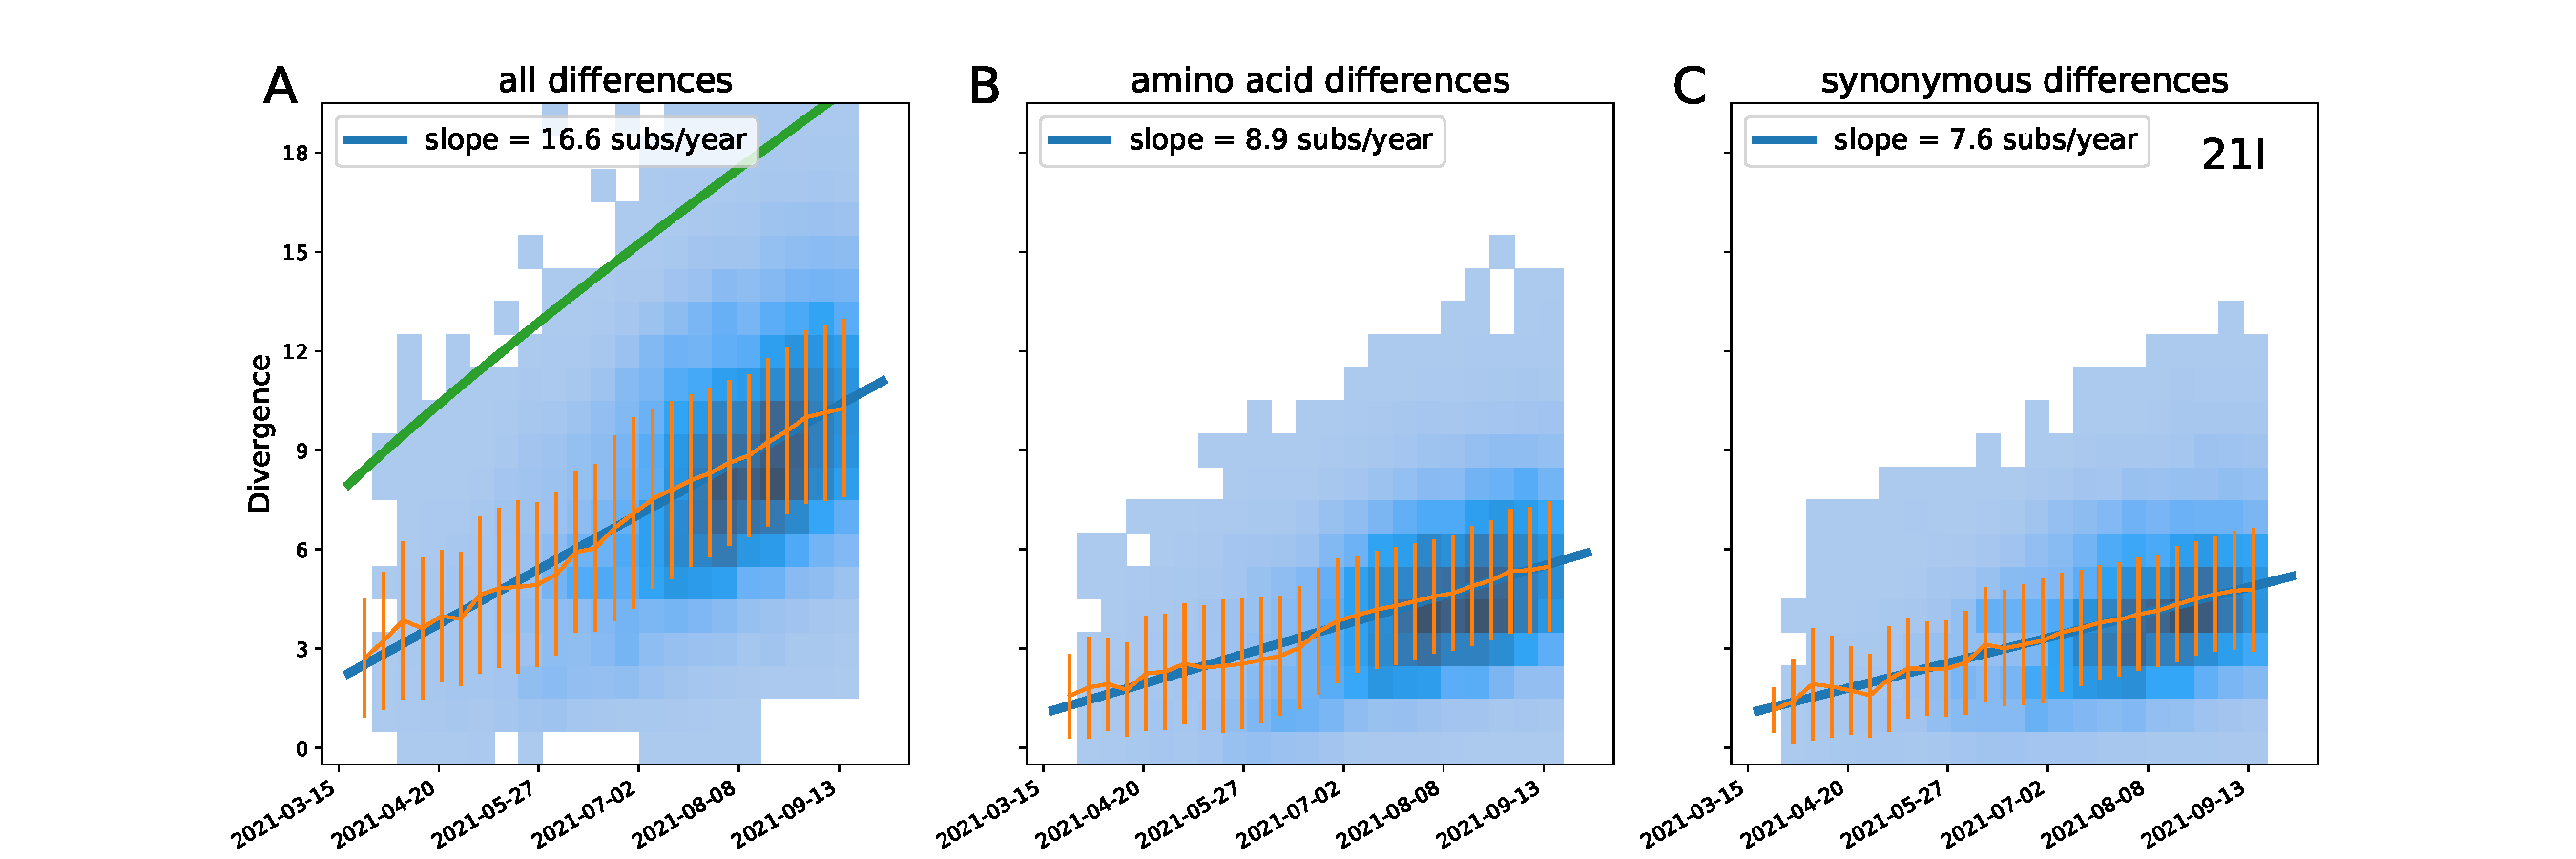
\includegraphics[width=0.8\textwidth]{figures/rtt/21I_rtt.pdf}
    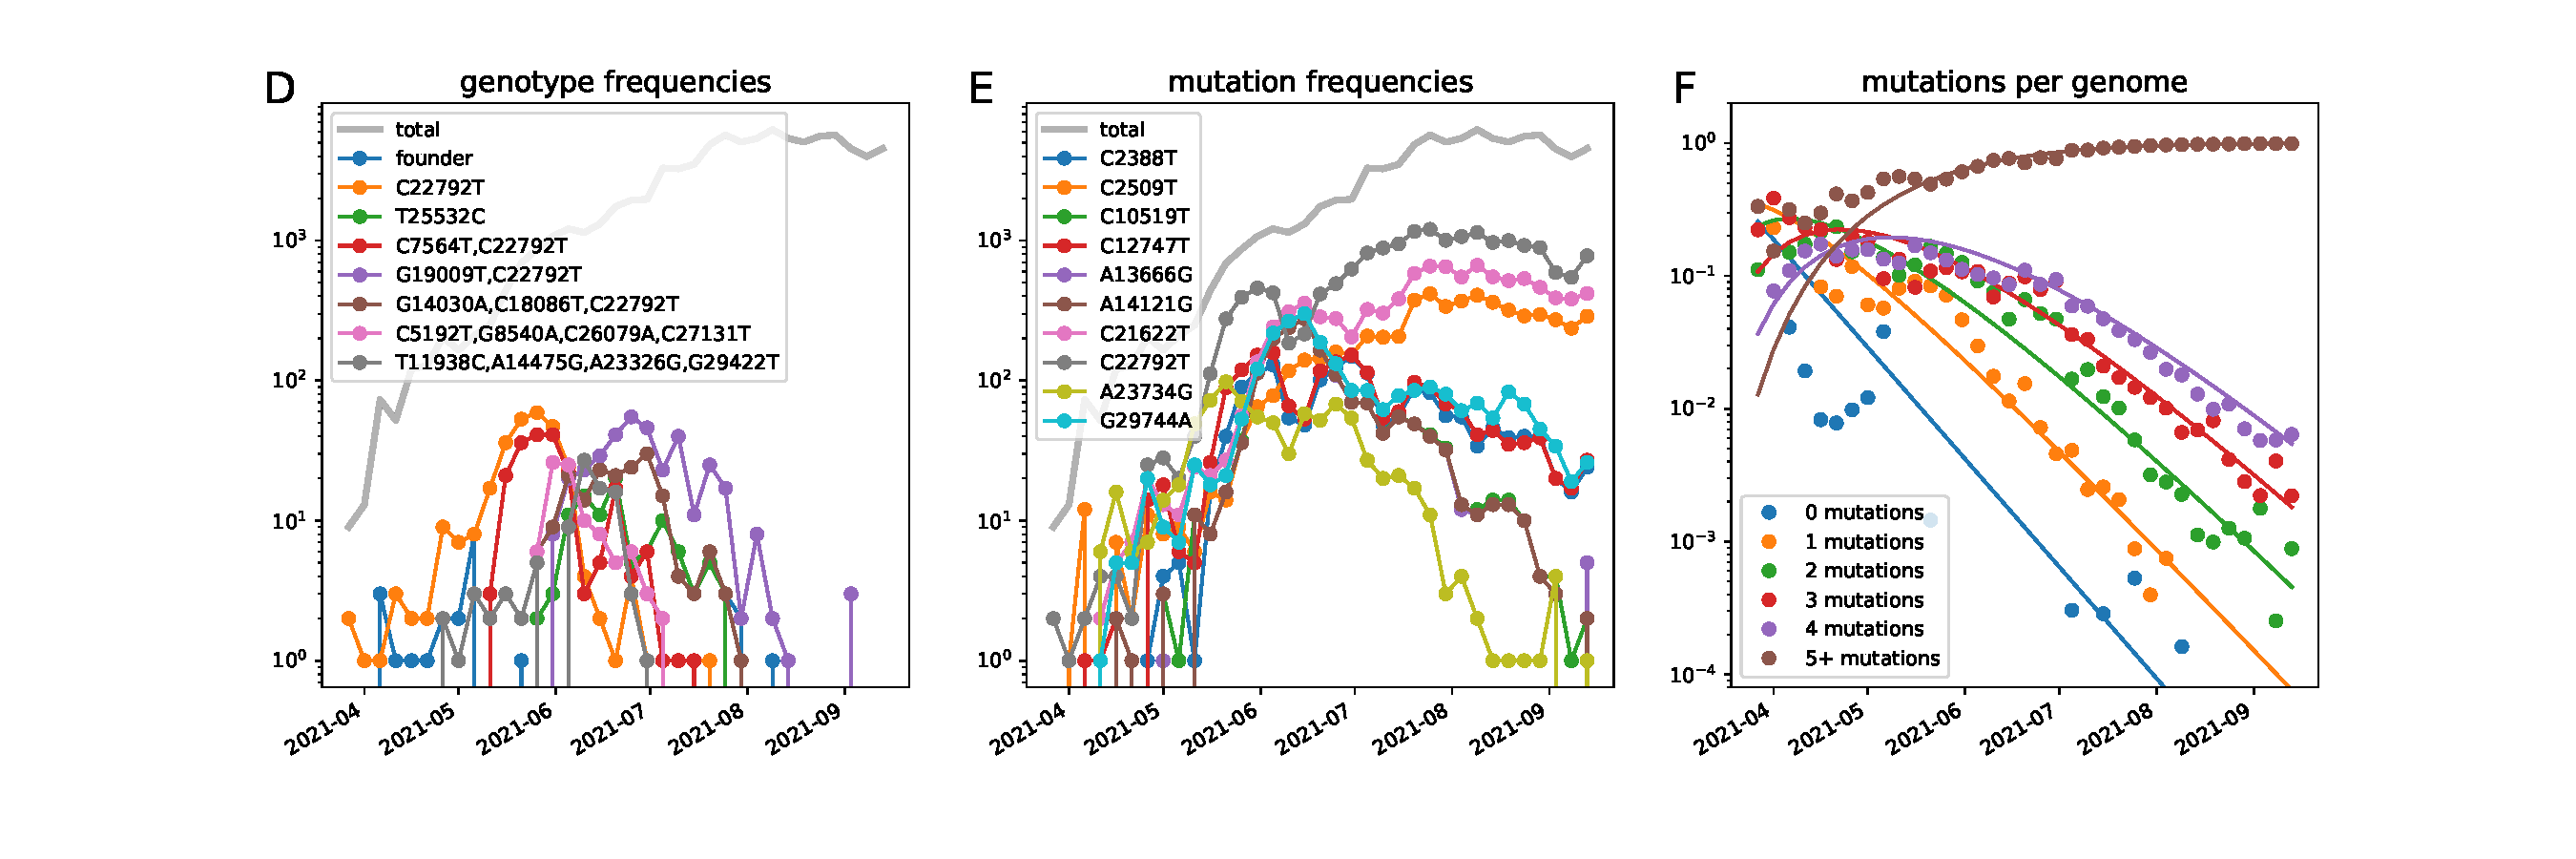
\includegraphics[width=0.8\textwidth]{figures/counts/21I_counts.pdf}
    \caption{{\bf Divergence increases linearly with time in clade 21I (Delta).}
    \label{fig:21I_divergence}}
\end{figure*}

\begin{figure*}[h]
    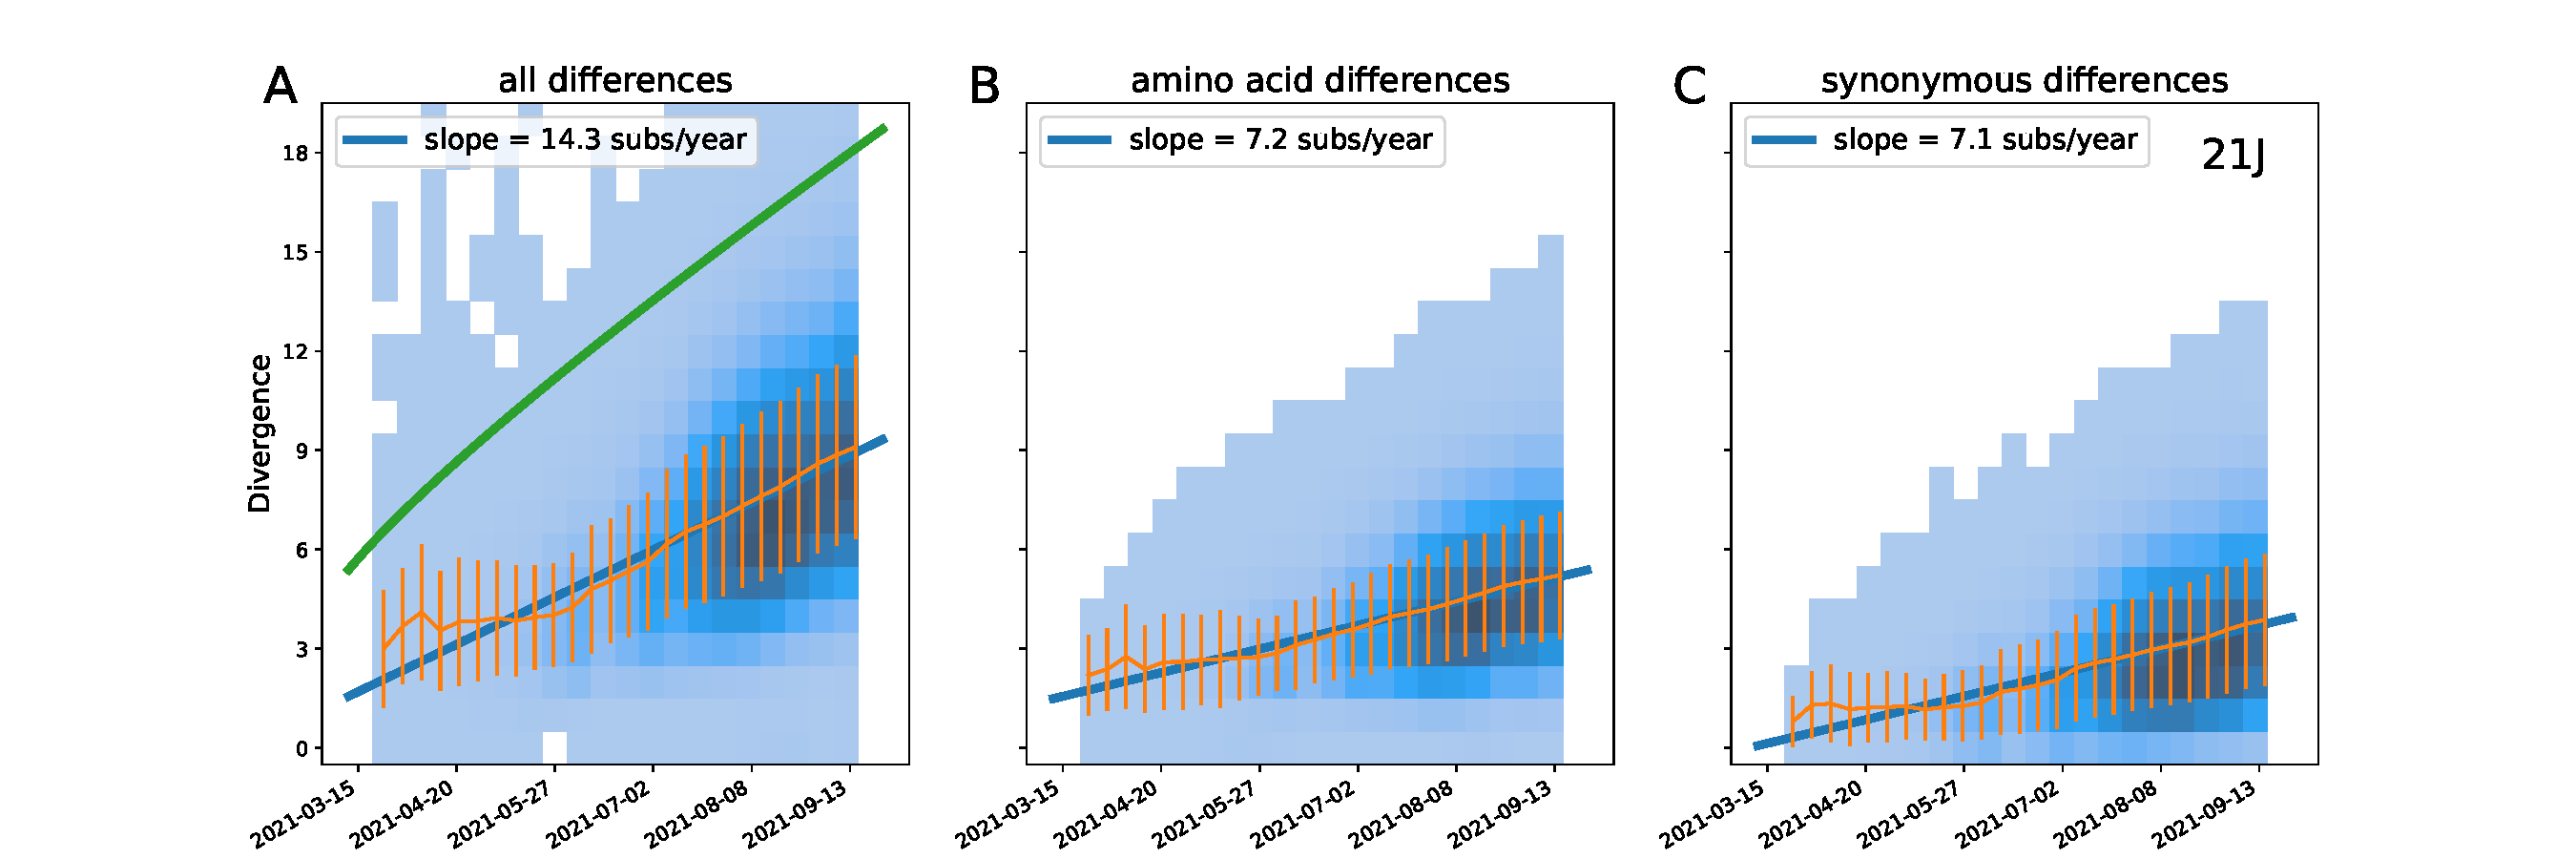
\includegraphics[width=0.8\textwidth]{figures/rtt/21J_rtt.pdf}
    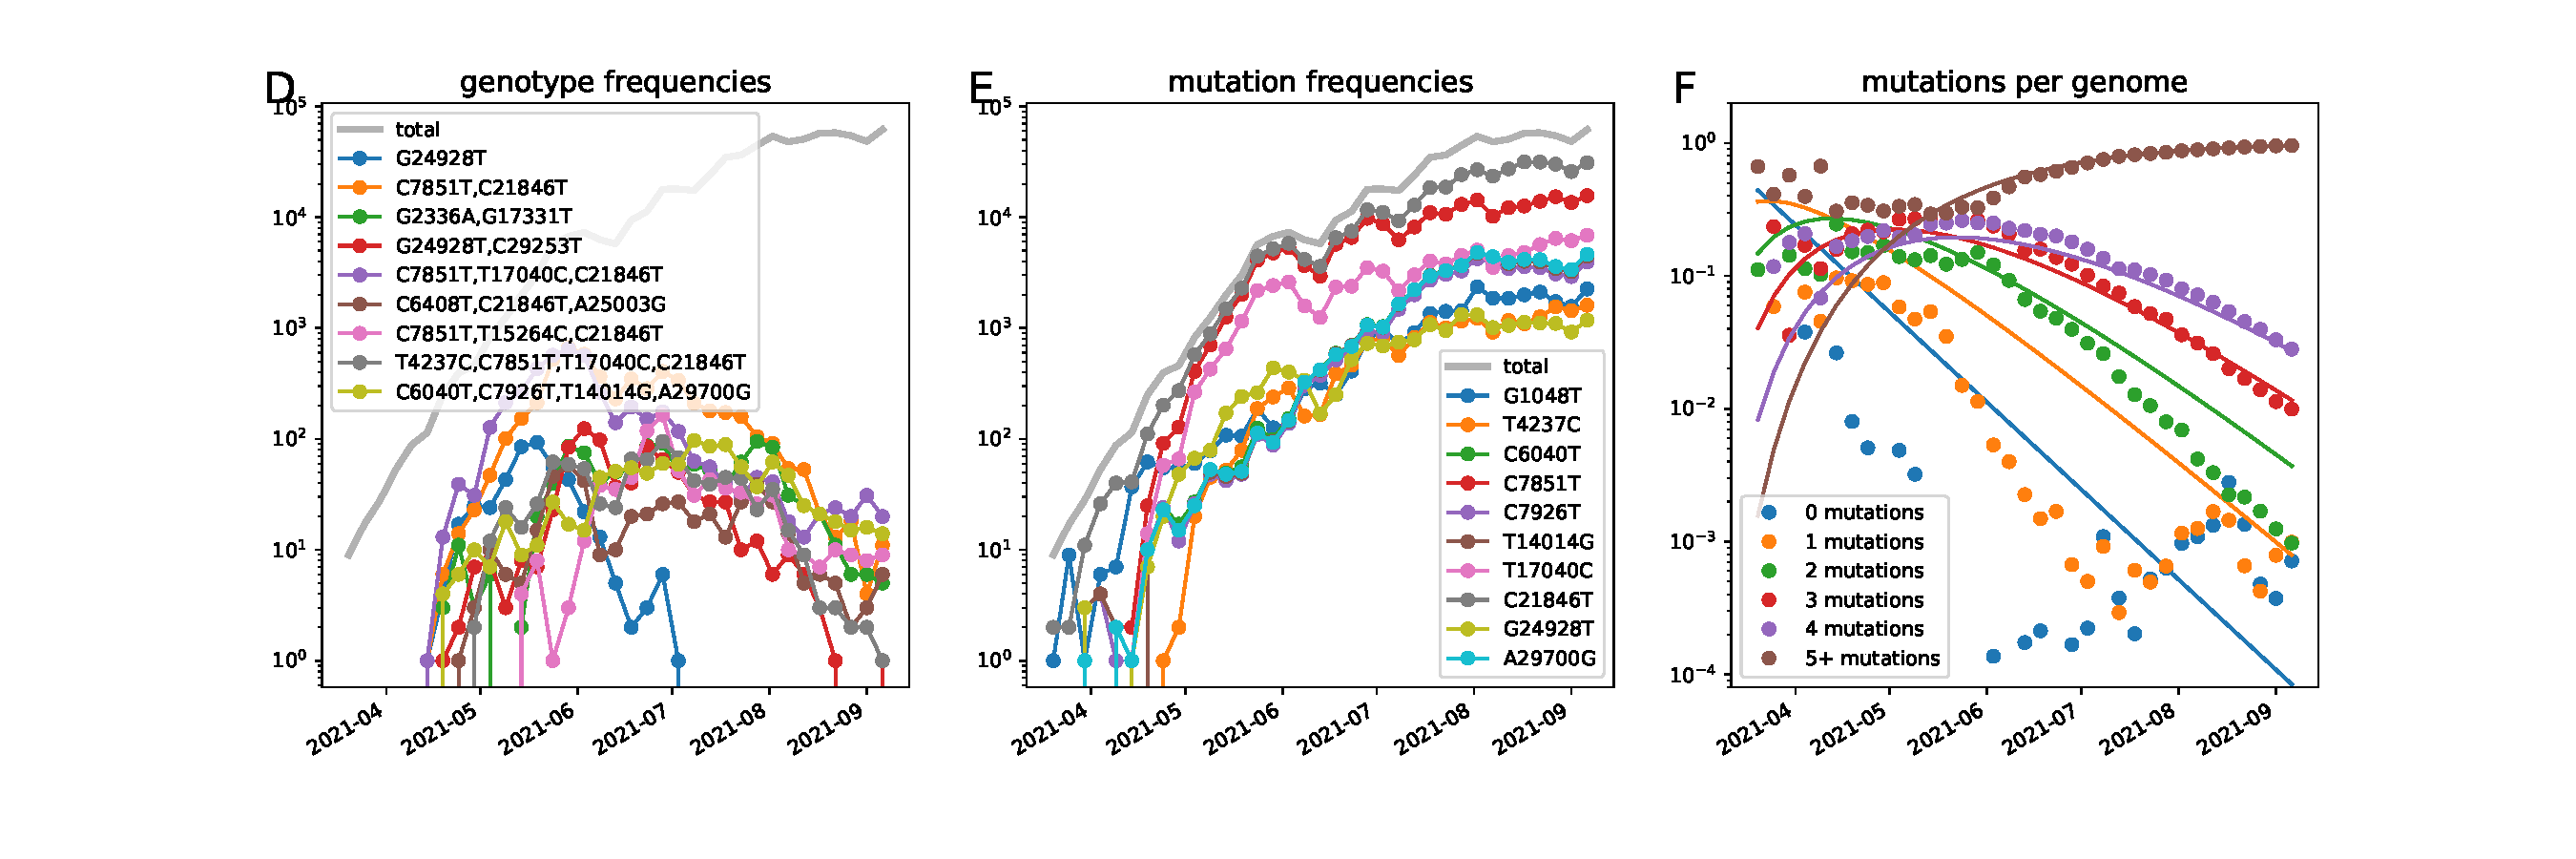
\includegraphics[width=0.8\textwidth]{figures/counts/21J_counts.pdf}
    \caption{{\bf Divergence increases linearly with time in clade 21J (Delta).}
    \label{fig:21J_divergence}}
\end{figure*}

\begin{figure*}[h]
    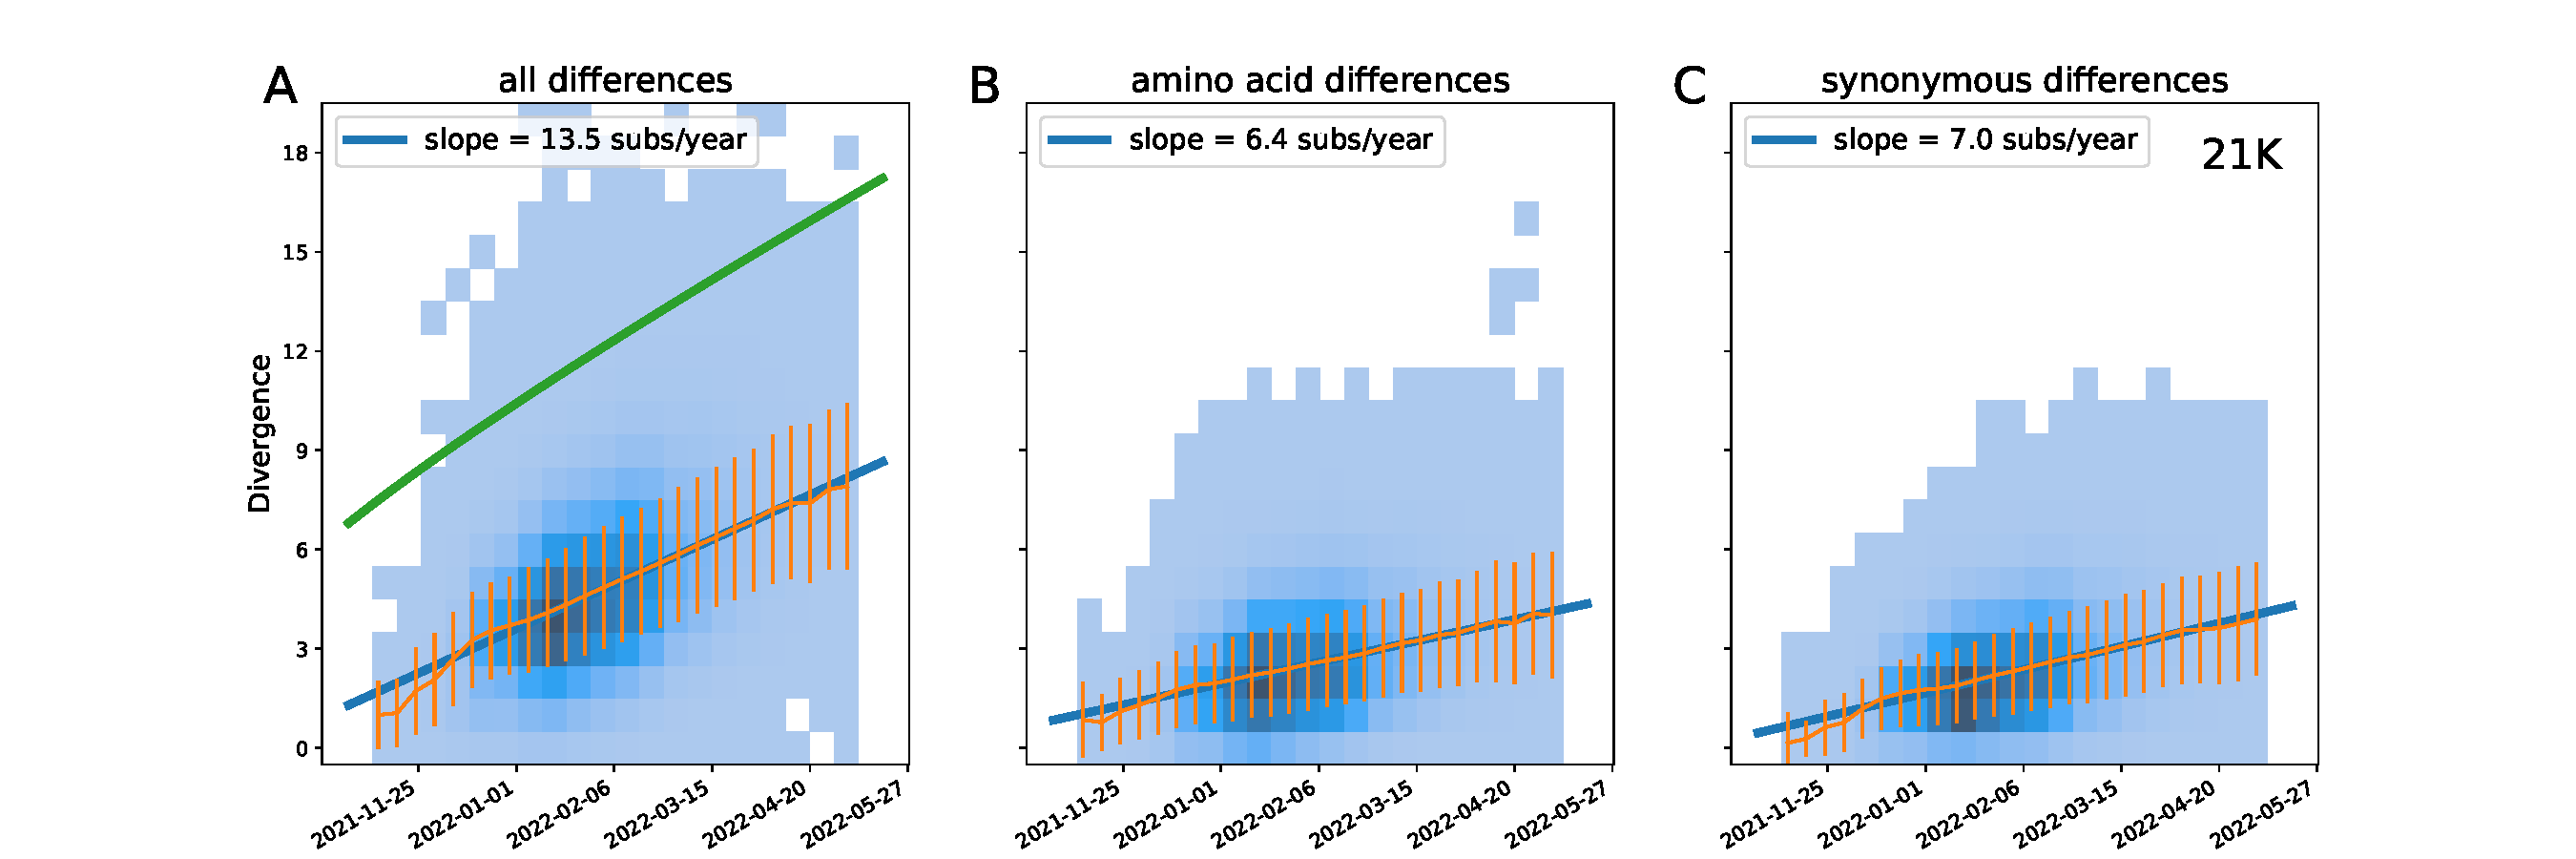
\includegraphics[width=0.8\textwidth]{figures/rtt/21K_rtt.pdf}
    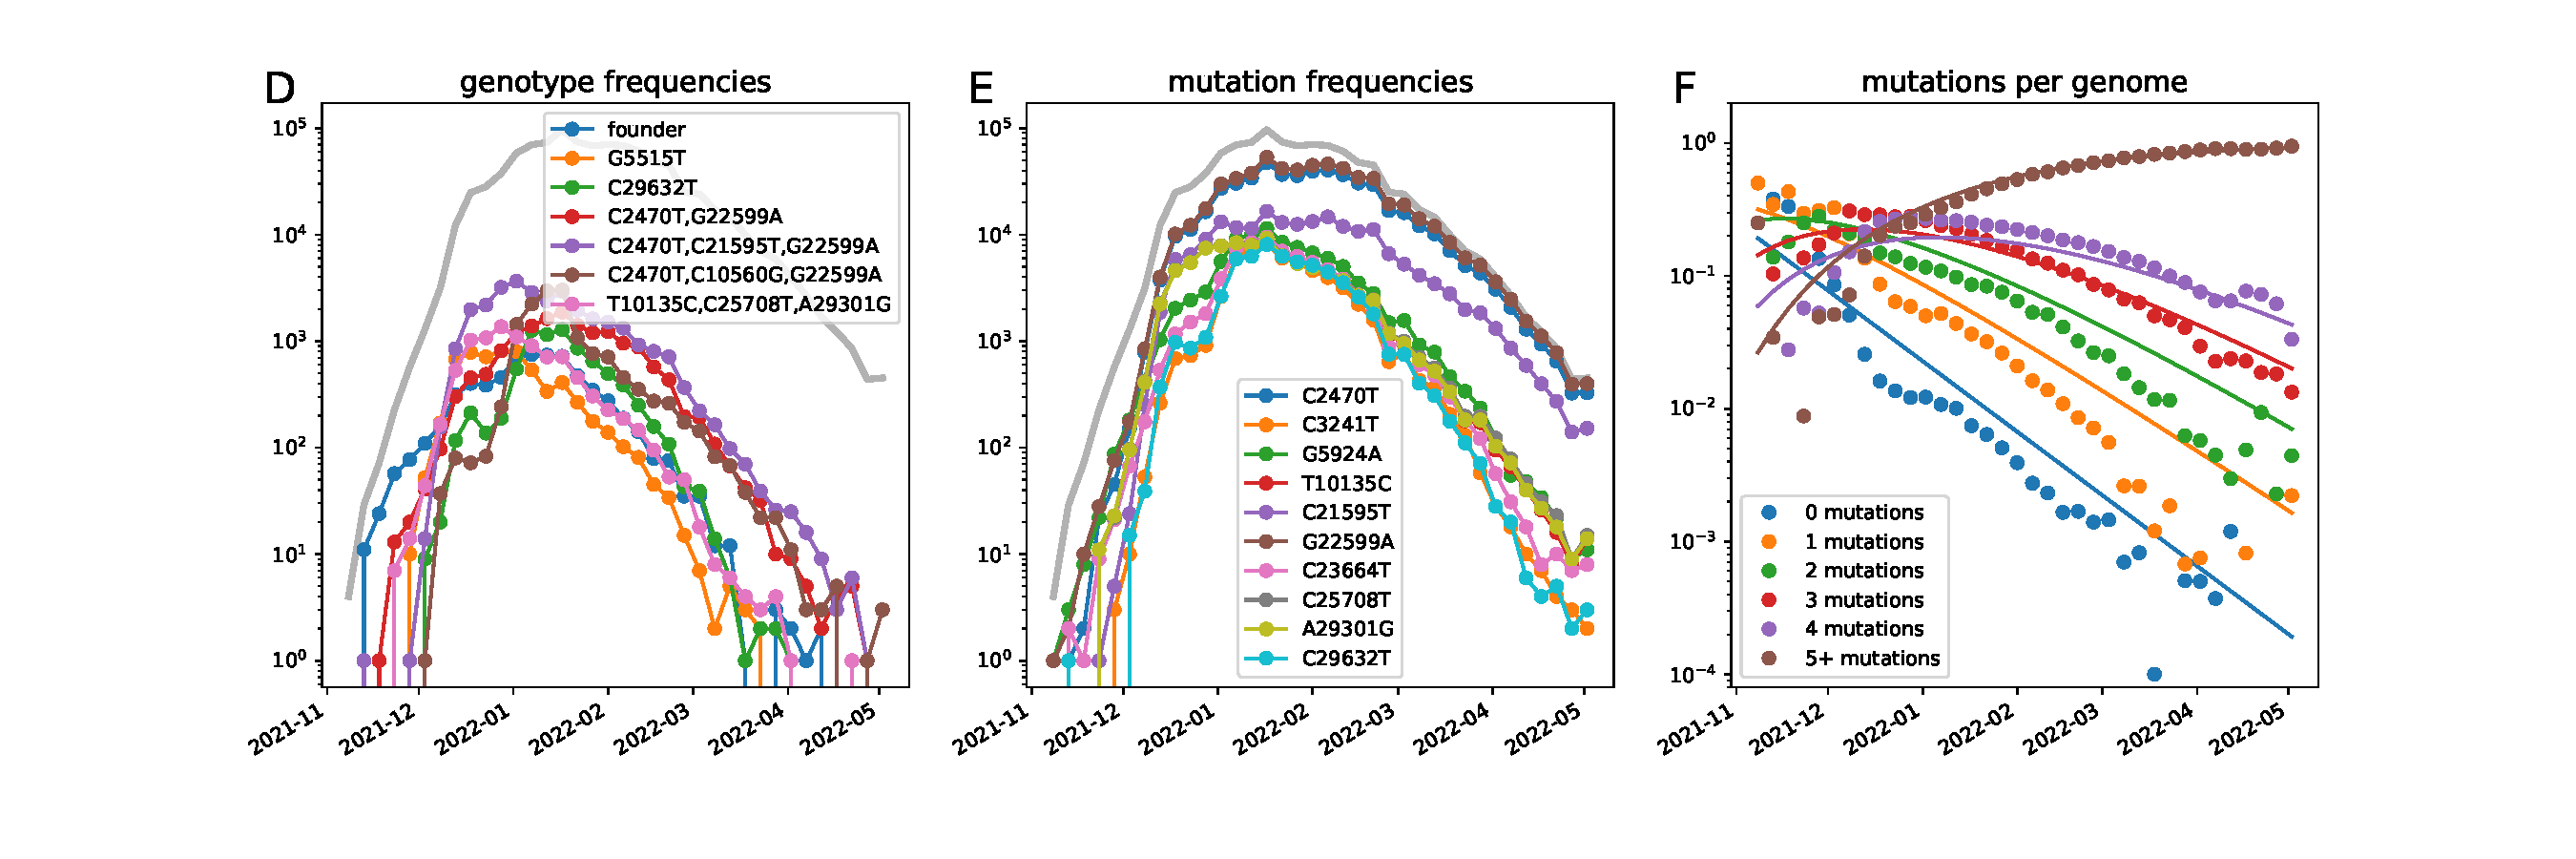
\includegraphics[width=0.8\textwidth]{figures/counts/21K_counts.pdf}
    \caption{{\bf Divergence increases linearly with time in clade 21K (Omicron).}
    \label{fig:21K_divergence}}
\end{figure*}

\begin{figure*}[h]
    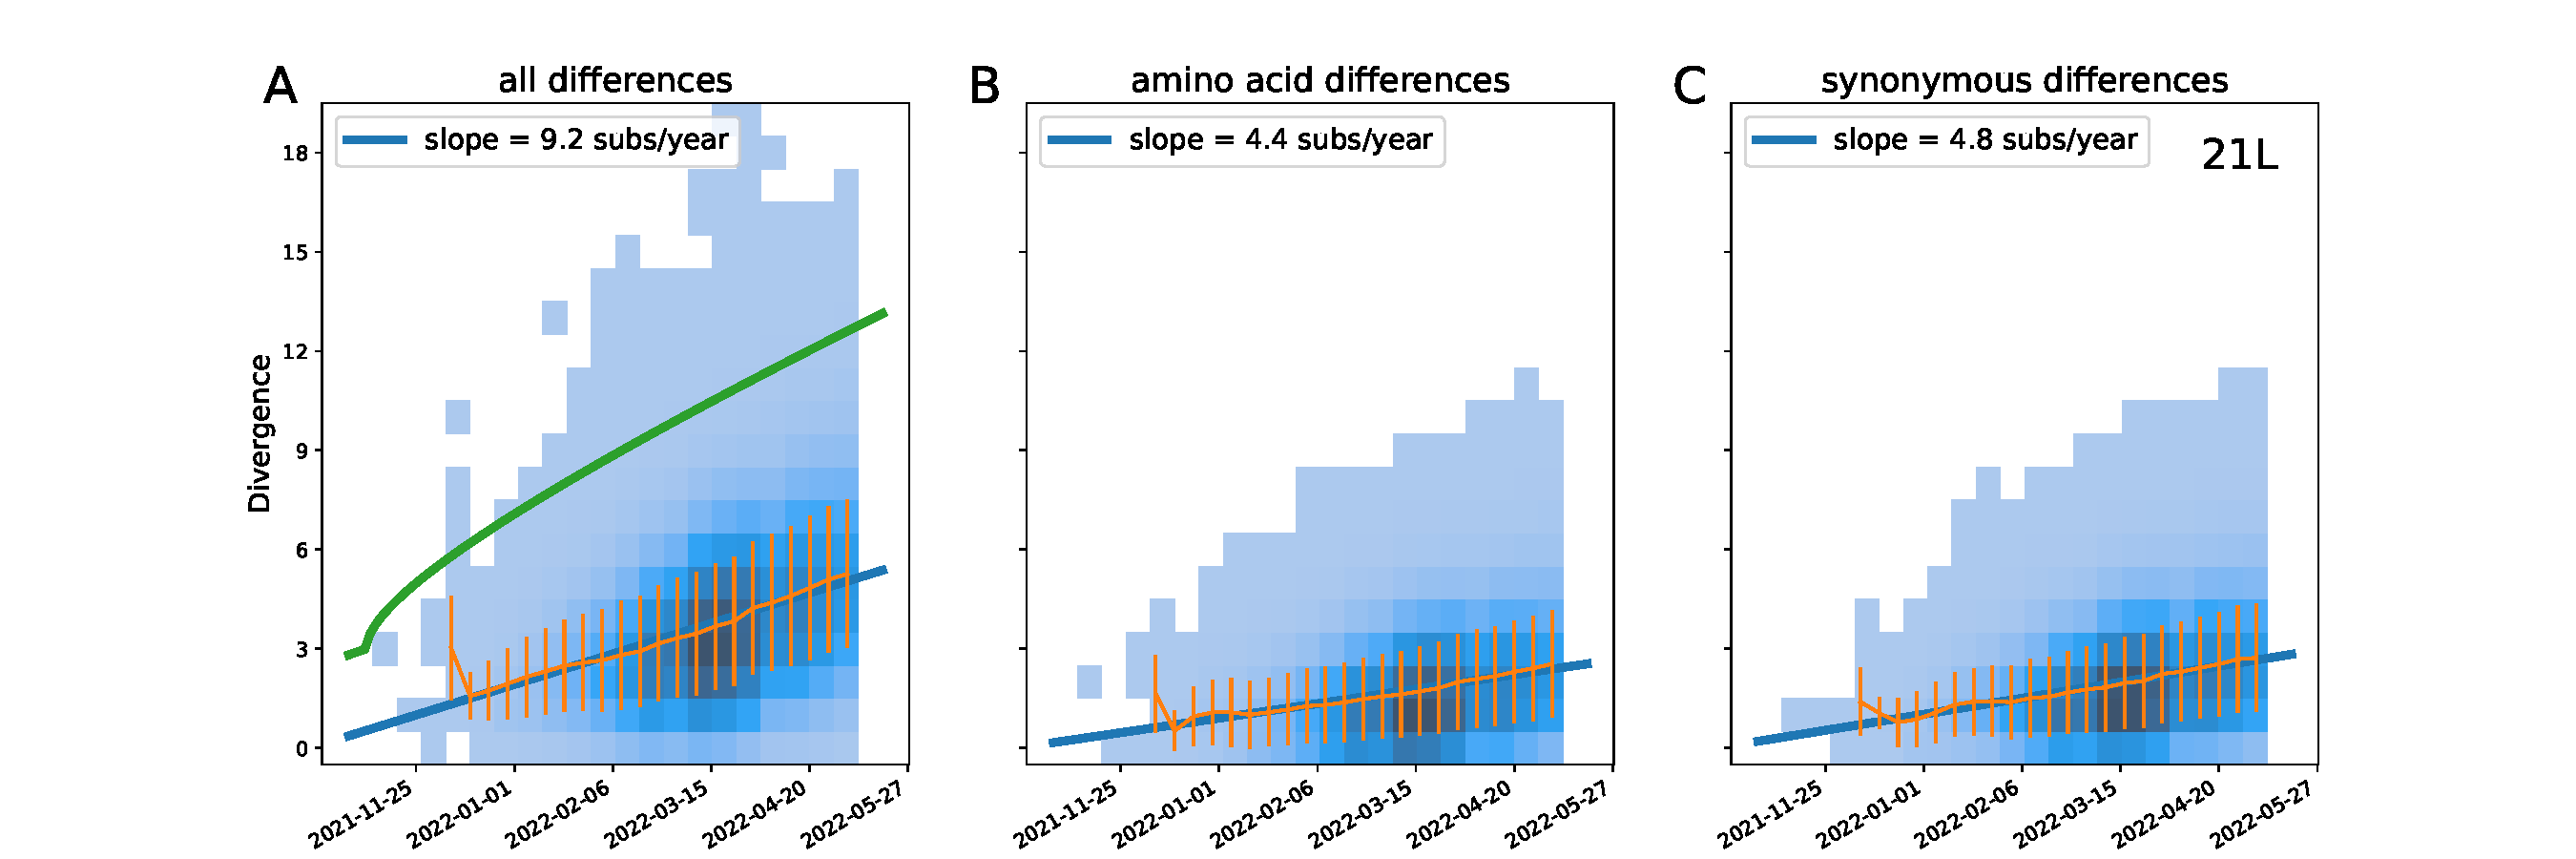
\includegraphics[width=0.8\textwidth]{figures/rtt/21L_rtt.pdf}
    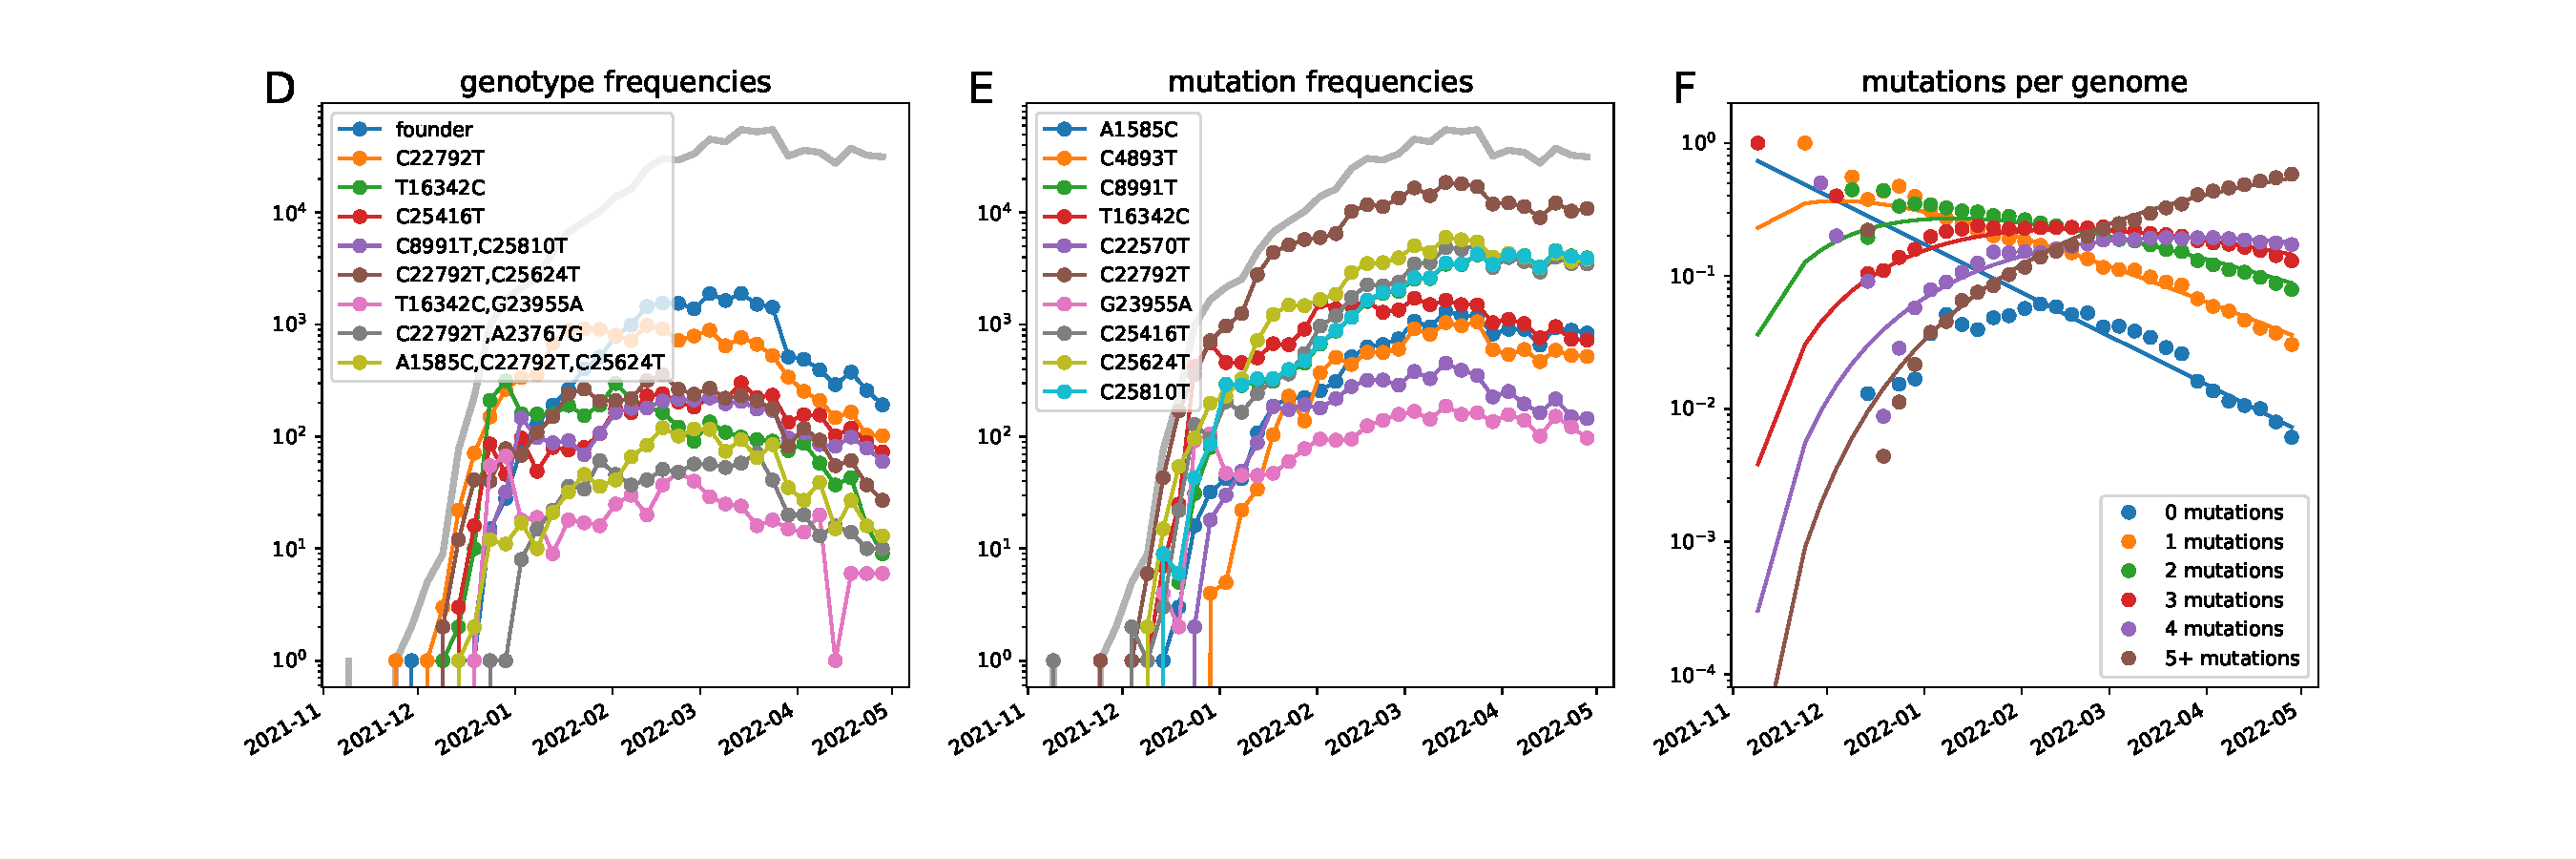
\includegraphics[width=0.8\textwidth]{figures/counts/21L_counts.pdf}
    \caption{{\bf Divergence increases linearly with time in clade 21L (Omicron).}
    \label{fig:21L_divergence}}
\end{figure*}

\begin{figure*}[h]
    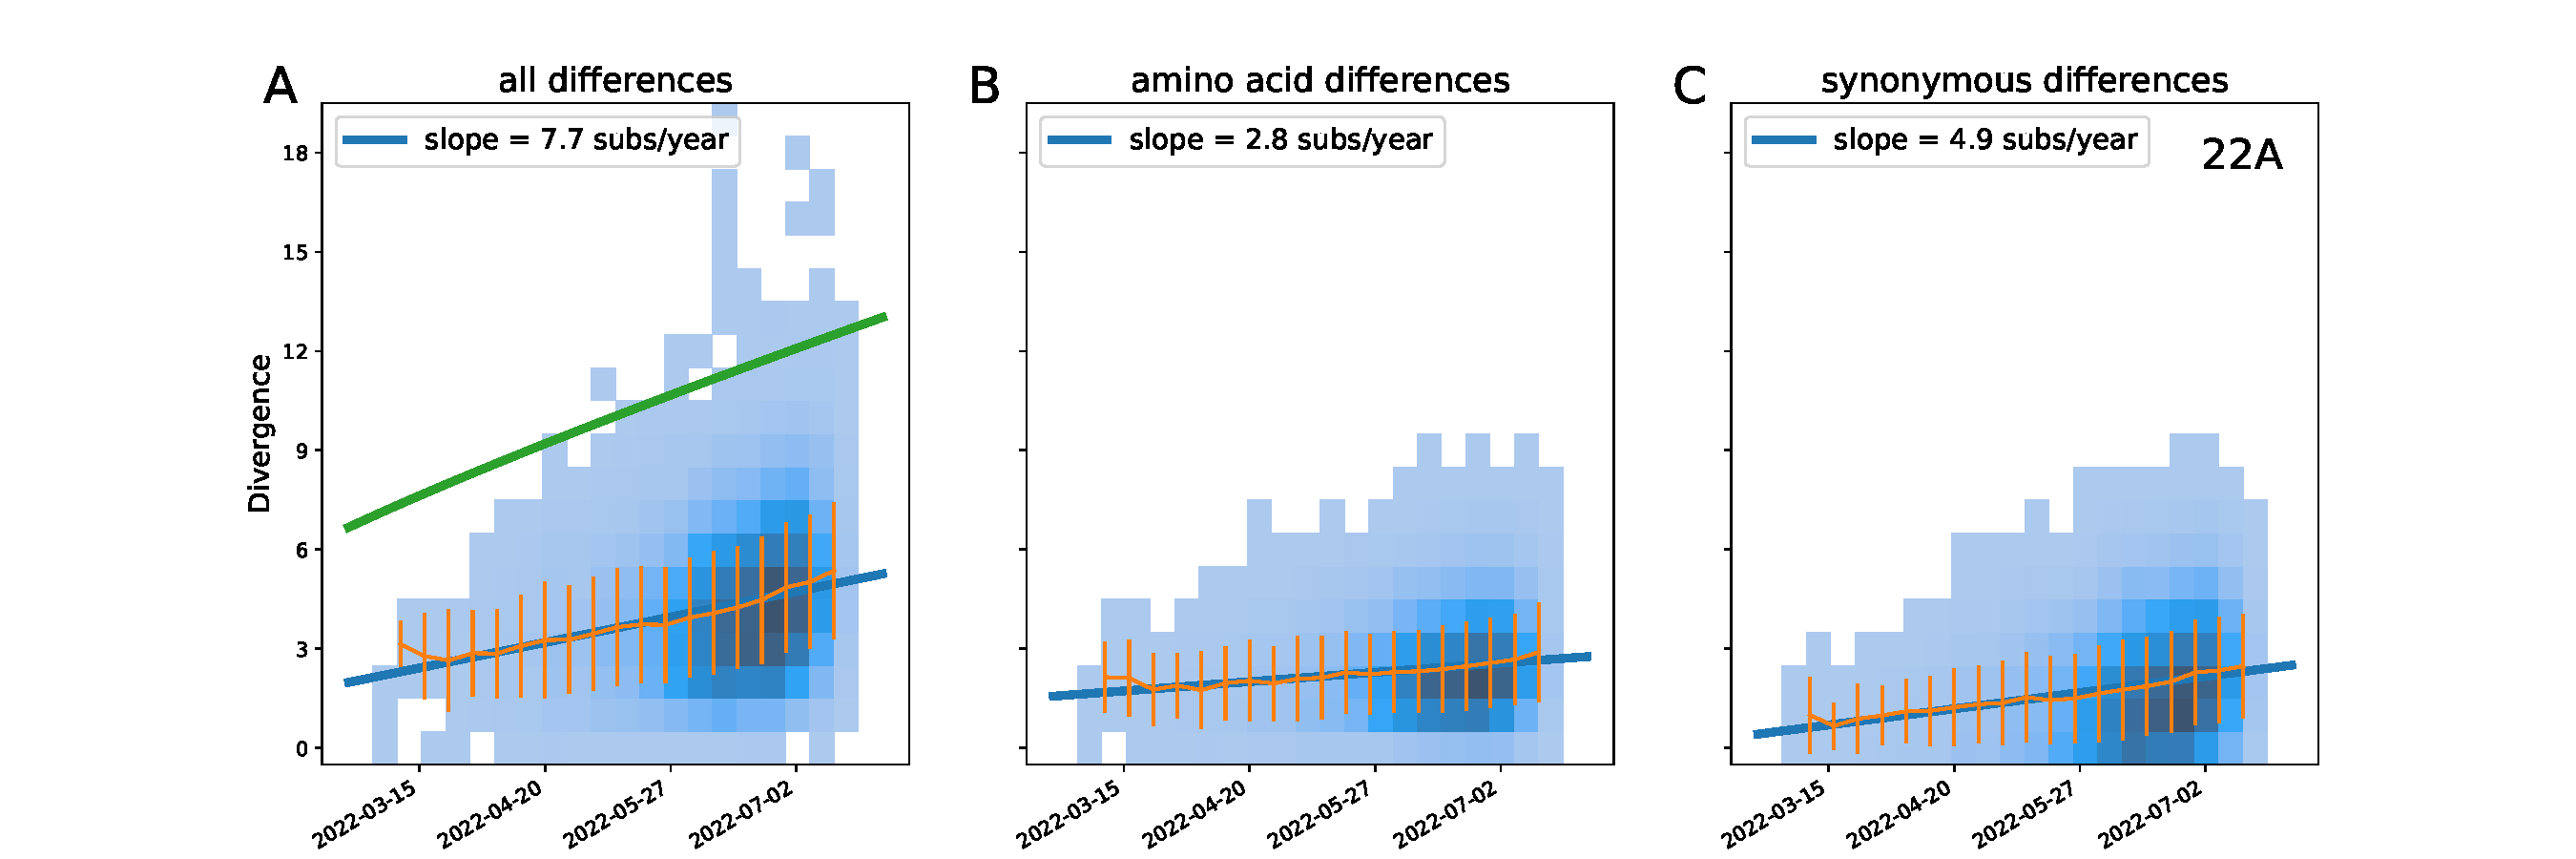
\includegraphics[width=0.8\textwidth]{figures/rtt/22A_rtt.pdf}
    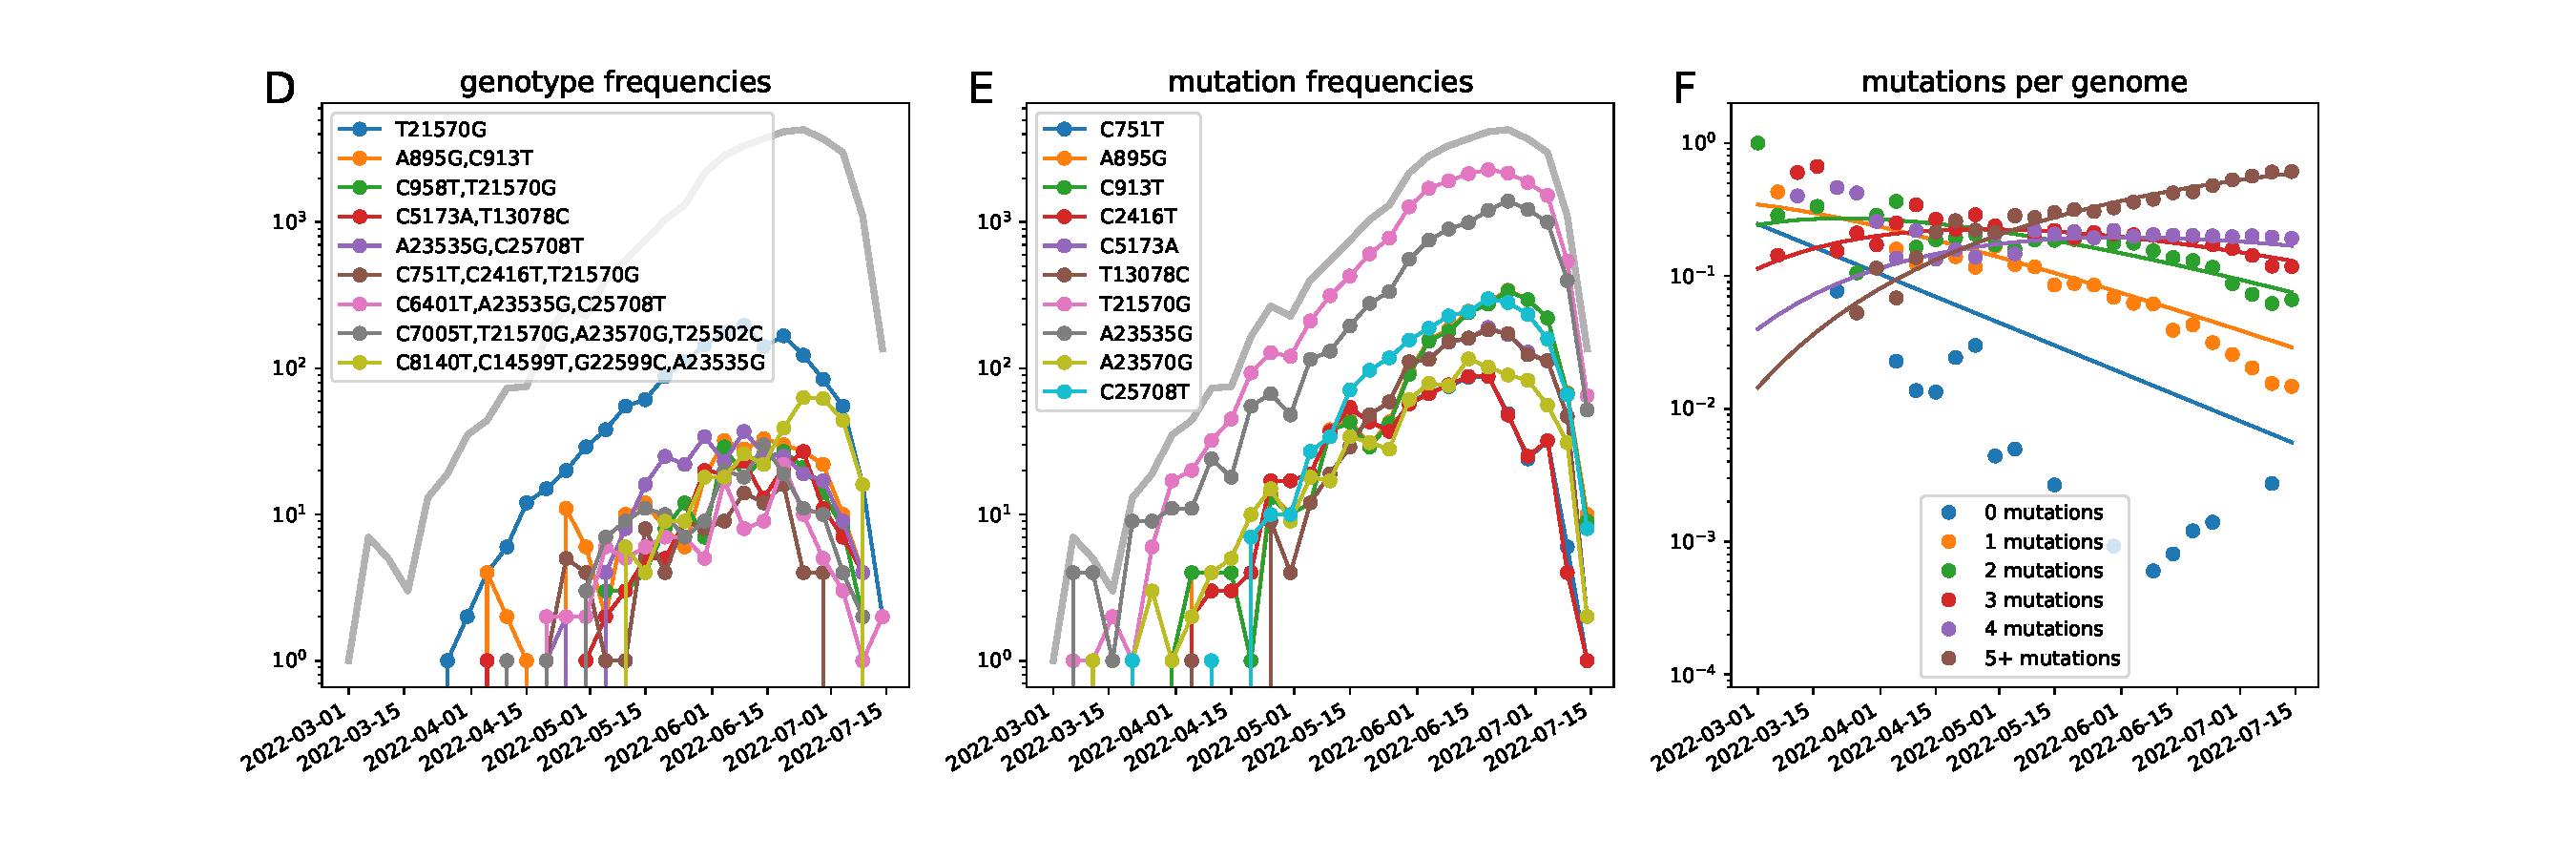
\includegraphics[width=0.8\textwidth]{figures/counts/22A_counts.pdf}
    \caption{{\bf Divergence increases linearly with time in clade 22A (Omicron).}
    \label{fig:22A_divergence}}
\end{figure*}

\begin{figure*}[h]
    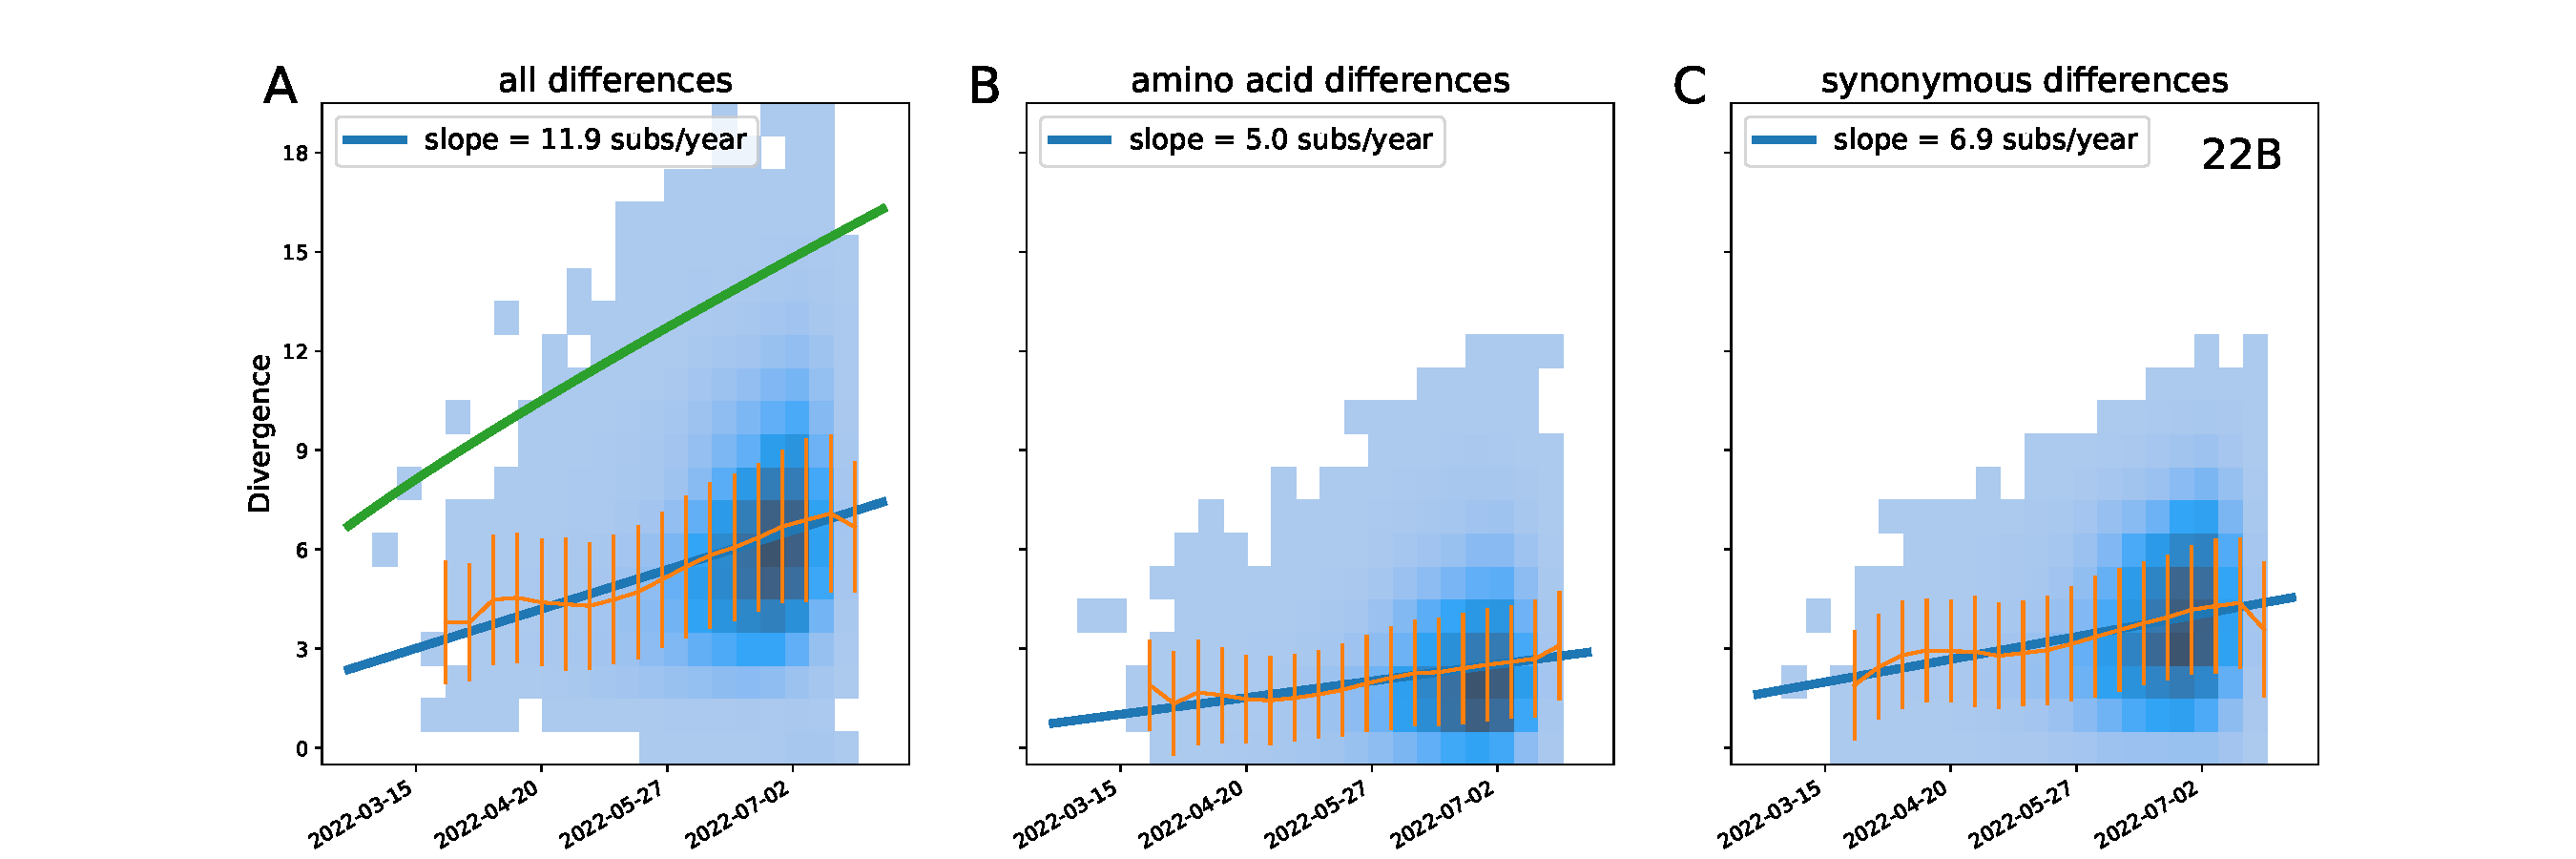
\includegraphics[width=0.8\textwidth]{figures/rtt/22B_rtt.pdf}
    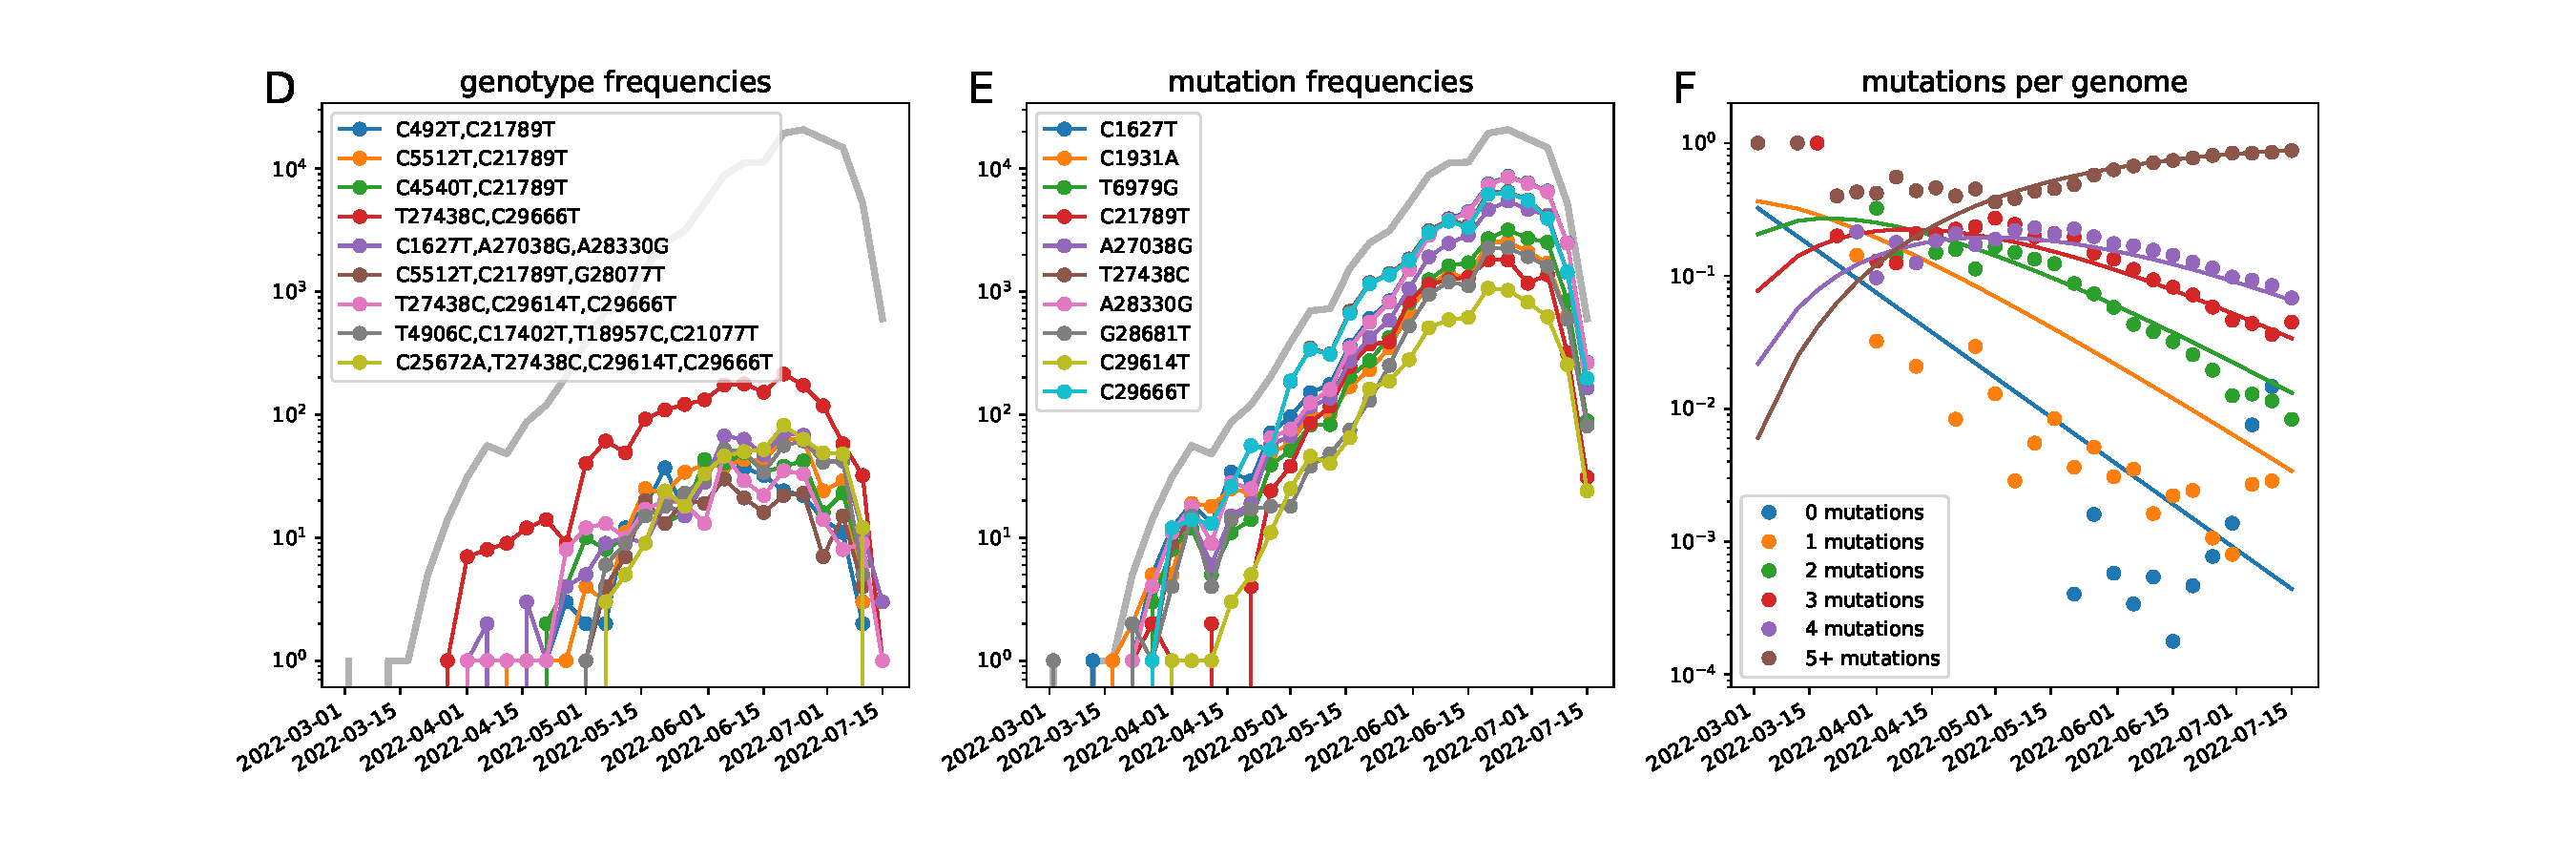
\includegraphics[width=0.8\textwidth]{figures/counts/22B_counts.pdf}
    \caption{{\bf Divergence increases linearly with time in clade 22B (Omicron).}
    \label{fig:22B_divergence}}
\end{figure*}
